\documentclass[11pt]{book}
\oddsidemargin 0in
\evensidemargin 0in
\marginparwidth 0in
\textheight 8in
\textwidth 6.5in
\topmargin 0in
\usepackage{amssymb,amsmath,amsthm,fancyhdr,supertabular,longtable,hhline}
\usepackage{colortbl}
\usepackage{import, multicol,boxedminipage}
\usepackage{chapterfolder}
\usepackage[metapost,truebbox]{mfpic}
\usepackage[pdflatex]{graphicx}
\usepackage{makeidx}
\usepackage[colorlinks, hyperindex, plainpages=false, linkcolor=blue, urlcolor=blue, pdfpagelabels]{hyperref}
\usepackage[all]{hypcap}
\usepackage{cancel}
\usepackage{sectsty}
\usepackage{textcomp}
\allsectionsfont{\mdseries \scshape}
\definecolor{ResultColor}{gray}{0.9}
\theoremstyle{definition}  % this prevents the text in definitions, theorems, and corollaries from being italicized
\newtheorem{defn}{Definition}[chapter]
\newtheorem{thm}{Theorem}[chapter]
\newtheorem{cor}[thm]{Corollary}
\newtheorem{eqn}{Equation}[chapter]
\newtheorem{ex}{Example}[section]
\setlength{\parindent}{0in}
\newcommand{\bbm}{\begin{boxedminipage}{6.41in}}
\newcommand{\ebm}{\end{boxedminipage}}
\newcounter{HW}
\newcounter{HWindent}

\begin{document}

\chapter{\sc Further Topics in Functions}

\section{Function Composition}

\mfpicnumber{1}

\opengraphsfile{FunctionComposition}

\setcounter{footnote}{0}

\label{FunctionComposition}

Before we embark upon any further adventures with functions, we need to take some time to gather our thoughts and gain some perspective.  Chapter \ref{RelationsandFunctions} first introduced us to functions in Section \ref{IntrotoFunctions}.  At that time, functions were specific kinds of relations - sets of points in the plane which passed the Vertical Line Test, Theorem \ref{VLT}.  In Section \ref{FunctionNotation}, we developed the idea that functions are processes - rules which match inputs to outputs - and this gave rise to the concepts of domain and range.  We spoke about how functions could be combined in Section \ref{FunctionArithmetic} using the four basic arithmetic operations, took a more detailed look at their graphs in Section \ref{GraphsofFunctions} and studied how their graphs behaved under certain classes of transformations in Section \ref{Transformations}.  In Chapter \ref{LinearQuadratic}, we took a closer look at three families of functions: linear functions (Section \ref{LinearFunctions}), absolute value functions\footnote{These were introduced, as you may recall, as piecewise-defined linear functions.} (Section \ref{AbsoluteValueFunctions}), and quadratic functions (Section \ref{QuadraticFunctions}).  Linear and quadratic functions were special cases of polynomial functions, which we studied in generality in Chapter \ref{Polynomials}. Chapter \ref{Polynomials} culminated with the Real Factorization Theorem, Theorem \ref{realfactorization}, which says that all polynomial functions with real coefficients can be thought of as products of linear and quadratic functions.  Our next step was to enlarge our field\footnote{This is a really bad math pun.} of study to rational functions in Chapter \ref{Rationals}.  Being quotients of polynomials, we can ultimately view this family of functions as being built up of linear and quadratic functions as well.  So in some sense, Chapters \ref{LinearQuadratic}, \ref{Polynomials}, and \ref{Rationals} can be thought of as an exhaustive study of linear and quadratic\footnote{If we broaden our concept of functions to allow for complex valued coefficients, the Complex Factorization Theorem, Theorem \ref{complexfactorization}, tells us every function we have studied thus far is a combination of linear functions.} functions and their arithmetic combinations as described in Section \ref{FunctionArithmetic}. We now wish to study other algebraic functions, such as $f(x) = \sqrt{x}$ and $g(x) = x^{2/3}$, and the purpose of the first two sections of this chapter is to see how these kinds of functions arise from polynomial and rational functions.  To that end, we first study a new way to combine functions as defined below.

\smallskip

\colorbox{ResultColor}{\bbm

\begin{defn} \label{functioncompositiondefn} Suppose $f$ and $g$ are two functions.  The \index{function ! composite ! definition of} \index{composite function ! definition of} \textbf{composite} of $g$ with $f$, denoted $g \circ f$, is defined by the formula $(g \circ f) (x) = g(f(x))$, provided $x$ is an element of the domain of $f$ and $f(x)$ is an element of the domain of $g$. 


\end{defn}
\ebm}

\smallskip

The quantity $g \circ f$ is also read `$g$ composed with $f$' or, more simply `$g$ of $f$.' At its most basic level, Definition \ref{functioncompositiondefn} tells us to obtain the formula for $\left(g \circ f\right)(x)$, we replace every occurrence of $x$ in the formula for $g(x)$ with the formula we have for $f(x)$.  If we take a step back and look at this from a procedural, `inputs and outputs' perspective, Defintion \ref{functioncompositiondefn} tells us  the output from $g \circ f$ is found by taking the output from $f$, $f(x)$,  and then making that the input to $g$.  The result, $g(f(x))$, is the output from $g \circ f$.  From this perspective, we see $g \circ f$ as a two step process taking an input $x$ and first applying the procedure $f$ then applying the procedure $g$.  Abstractly, we have

\begin{center}

\footnotesize

\begin{mfpic}[10]{-10}{20}{-10}{10}
\tlabel[cc](-2,6){$f$}
\tlabel[cc](11,6){$g$}
\tlabel[cc](4.5,-6){$g \circ f$}
\tlabel[cc](-9,-1){$x$}
\tlabel[cc](4,-1){$f(x)$}
\tlabel[cc](18,-2){$g(f(x))$}
\point[2pt]{(-9,0), (4,0), (18,0)} 
\sclosed \curve{(-6,4), (-12,0), (-6,-5), (-3,0)}
\sclosed \curve{(1,3), (6,0), (5,-4)}
\sclosed \curve{(18,3), (15,0), (18,-5), (20,0)}
\penwd{0.75pt}
\arrow \curve{(-8.9,0.25), (-2,5), (3.9,0.25)}
\arrow \curve{(4.1,0.25), (11,5), (17.9,0.25)}
\arrow \curve{(-8.9,-0.25), (4.5,-5), (17.9,-0.25)}
\end{mfpic}

\end{center}

\normalsize

In the expression $g(f(x))$, the function $f$ is often called the `inside' function while $g$ is often called the `outside' function.  There are two ways to go about evaluating composite functions - `inside out' and `outside in' - depending on which function we replace with its formula first.  Both ways are  demonstrated in the following example.  

\begin{ex}  Let $f(x) = x^2-4x$, $g(x) = 2-\sqrt{x+3}$, and $h(x) = \dfrac{2x}{x+1}$.  

In numbers \ref{fcexvalfirst} - \ref{fcexvallast}, find the indicated function value.

\begin{multicols}{3}
\begin{enumerate}

\item  $(g \circ f)(1)$ \label{fcexvalfirst}

\item  $(f \circ g)(1)$

\item  $(g \circ g)(6)$ \label{fcexvallast}

\setcounter{HW}{\value{enumi}}
\end{enumerate}
\end{multicols}





In numbers \ref{fcexformfirst} - \ref{fcexformlast}, find and simplify the indicated composite functions.  State the domain of each.

\begin{multicols}{4}
\begin{enumerate}
\setcounter{enumi}{\value{HW}}

\item  $(g \circ f)(x)$ \label{fcexformfirst}

\item  $(f \circ g)(x)$

\item  $(g \circ h)(x)$

\item  $(h \circ g)(x)$

\setcounter{HW}{\value{enumi}}
\end{enumerate}
\end{multicols}

\begin{multicols}{4}
\begin{enumerate}
\setcounter{enumi}{\value{HW}}

\item  $(h \circ h)(x)$

\item  $(h \circ (g \circ f))(x)$ 

\item  $((h \circ g) \circ f)(x)$ \label{fcexformlast}

\end{enumerate}
\end{multicols}

{\bf Solution.}  
\begin{enumerate}

\item  Using Definition \ref{functioncompositiondefn}, $(g \circ f)(1) = g(f(1))$.  We find $f(1) = -3$, so \[(g \circ f)(1) = g(f(1)) = g(-3) = 2 \]

\item As before, we use Definition \ref{functioncompositiondefn} to write $(f \circ g)(1) = f(g(1))$.  We find $g(1) = 0$, so \[(f \circ g)(1) = f(g(1)) = f(0) = 0 \] 

\item  Once more, Definition \ref{functioncompositiondefn} tells us $(g \circ g)(6) = g(g(6))$.  That is, we evaluate $g$ at $6$, then plug that result back into $g$. Since $g(6) = -1$,  \[(g \circ g)(6) = g(g(6)) = g(-1) = 2-\sqrt{2} \]


\item  By definition, $(g \circ f)(x) = g(f(x))$. We now illustrate \textit{two} ways to approach this problem.

\begin{itemize}

\item  \textit{inside out}:  We insert the expression $f(x)$ into $g$ first to get  \[(g \circ f)(x) = g(f(x)) = g\left(x^2-4x\right) = 2 - \sqrt{\left(x^2-4x\right)+3} = 2 - \sqrt{x^2-4x+3}\] Hence, $(g \circ f)(x) = 2 - \sqrt{x^2-4x+3}$.

\item  \textit{outside in}:  We use the formula for $g$ first to get  \[(g \circ f)(x) = g(f(x)) = 2 - \sqrt{f(x)+3}  = 2 - \sqrt{\left(x^2-4x\right)+3} = 2 - \sqrt{x^2-4x+3}\] We get the same answer as before,  $(g \circ f)(x) = 2 - \sqrt{x^2-4x+3}$.

\end{itemize} 

To find the domain of $g \circ f$, we need to find the elements in the domain of $f$ whose outputs $f(x)$ are in the domain of $g$.  We accomplish this by following the rule set forth in Section \ref{FunctionNotation}, that is, we find the domain \textit{before} we simplify.  To that end, we examine $(g \circ f)(x) = 2 - \sqrt{\left(x^2-4x\right)+3}$.  To keep the square root happy, we solve the inequality $x^2-4x+3 \geq 0$ by creating a sign diagram.  If we let $r(x) = x^2-4x+3$, we find the zeros of $r$ to be $x = 1$ and $x = 3$.  We obtain

\begin{center}

\begin{mfpic}[10]{-5}{5}{-1}{2}
\arrow \reverse \arrow \polyline{(-5,0),(5,0)}
\xmarks{-2,2}
\tlpointsep{6pt}
\axislabels {x}{{$1$} -2, {$3$} 2}
\tlabel[cc](-3.5,1){$(+)$}
\tlabel[cc](-2,1){$0$}
\tlabel[cc](0,1){$(-)$}
\tlabel[cc](2,1){$0$}
\tlabel[cc](3.5,1){$(+)$}
\end{mfpic}

\end{center}

Our solution to $x^2-4x+3 \geq 0$, and hence the domain of $g \circ f$, is $(-\infty, 1] \cup [3,\infty)$.

\item  To find $(f \circ g)(x)$, we find $f(g(x))$. 

\begin{itemize}

\item  \textit{inside out}: We insert the expression $g(x)$ into $f$ first to get  
\begin{longtable}{rclr} $(f \circ g)(x)$ & = & $f(g(x))$ = $f\left(2-\sqrt{x+3}\right)$ & \\ [2pt]
 & = & $\left(2-\sqrt{x+3}\right)^2 - 4\left(2-\sqrt{x+3}\right)$ & \\[2pt] 
 & = & $4 - 4\sqrt{x+3} + \left(\sqrt{x+3}\right)^2 - 8 + 4 \sqrt{x+3}$ & \\ [2pt]
 & = & $4 + x+3 - 8$ & \\ 
 & = & $x-1$ & \\
 \end{longtable}

\item  \textit{outside in}:  We use the formula for $f(x)$ first to get
\begin{longtable}{rclr} $(f \circ g)(x)$ & = & $f(g(x))$ = $\left(g(x)\right)^2 - 4\left(g(x)\right)$& \\ [2pt]
 & = & $\left(2-\sqrt{x+3}\right)^2 - 4\left(2-\sqrt{x+3}\right)$ & \\[2pt] 
 & = & $x-1$ & same algebra as before \\
 \end{longtable}

\end{itemize}

Thus we get $(f \circ g)(x) = x-1$.  To find the domain of $(f \circ g)$, we look to the step before we did any simplification and find $(f \circ g)(x) = \left(2-\sqrt{x+3}\right)^2 - 4\left(2-\sqrt{x+3}\right)$.  To keep the square root happy, we set $x+3 \geq 0$ and find our domain to be $[-3, \infty)$.  



\item  To find $(g \circ h)(x)$, we compute $g(h(x))$. 

\begin{itemize}

\item  \textit{inside out}: We insert the expression $h(x)$ into $g$ first to get 
\begin{longtable}{rclr} $(g \circ h)(x)$ & = & $g(h(x))$ = $g\left(\dfrac{2x}{x+1}\right)$  & \\ [12pt]
 & = & $2 - \sqrt{\left(\dfrac{2x}{x+1}\right)+3}$ & \\[12pt] 
 & = & $2 - \sqrt{\dfrac{2x}{x+1} + \dfrac{3(x+1)}{x+1}}$ & get common denominators\\ [12pt]
 & = & $2 - \sqrt{\dfrac{5x+3}{x+1}}$ & \\
 \end{longtable}

\item  \textit{outside in}:  We use the formula for $g(x)$ first to get
\begin{longtable}{rclr} $(g \circ h)(x)$ & = & $g(h(x))$ = $2 - \sqrt{h(x)+3}$& \\ [2pt]
  & = & $2 - \sqrt{\left(\dfrac{2x}{x+1}\right)+3}$ & \\[12pt] 
 & = & $2 - \sqrt{\dfrac{5x+3}{x+1}}$ & get common denominators as before\\
 \end{longtable}

\end{itemize}

To find the domain of $(g \circ h)$, we look to the step before we began to simplify: \[(g \circ h)(x) = 2 - \sqrt{\left(\frac{2x}{x+1}\right)+3}\]  To avoid division by zero, we need $x \neq -1$. To keep the radical happy, we need to solve \[\frac{2x}{x+1} +3  = \frac{5x+3}{x+1}\geq 0\] Defining $r(x) = \frac{5x+3}{x+1}$, we see $r$ is undefined at $x=-1$ and $r(x) = 0$ at $x = -\frac{3}{5}$. We get

\begin{center}

\begin{mfpic}[10]{-5}{5}{-1}{2}
\arrow \reverse \arrow \polyline{(-5,0),(5,0)}
\xmarks{-2,2}
\tlpointsep{7pt}
\axislabels {x}{{$-1 \hspace{7pt}$} -2, {$-\frac{3}{5} \hspace{7pt}$} 2}
\tlabel[cc](-3.5,1){$(+)$}
\tlabel[cc](-2,1){\textinterrobang}
\tlabel[cc](0,1){$(-)$}
\tlabel[cc](2,1){$0$}
\tlabel[cc](3.5,1){$(+)$}
\end{mfpic}

\end{center}

Our domain is $(-\infty, -1) \cup \left[-\frac{3}{5}, \infty\right)$.

\item  We find $(h \circ g)(x)$ by finding $h(g(x))$.

\begin{itemize}

\item  \textit{inside out}: We insert the expression $g(x)$ into $h$ first to get
\begin{longtable}{rclr} $(h \circ g)(x)$ & = & $h(g(x))$ =$h\left(2-\sqrt{x+3}\right)$ & \\ [2pt]
 & = & $\dfrac{2 \left(2-\sqrt{x+3} \right)}{\left(2-\sqrt{x+3}\right)+1}$ & \\[12pt] 
 & = & $\dfrac{4-2\sqrt{x+3}}{3-\sqrt{x+3}}$ & \\
  \end{longtable}

\item  \textit{outside in}:  We use the formula for $h(x)$ first to get
\begin{longtable}{rclr} $(h \circ g)(x)$ & = & $h(g(x))$ = $\dfrac{2 \left(g(x)\right)}{\left( g(x)\right) + 1}$ & \\ [12pt]
 & = & $\dfrac{2 \left(2-\sqrt{x+3} \right)}{\left(2-\sqrt{x+3}\right)+1}$ & \\[12pt] 
 & = & $\dfrac{4-2\sqrt{x+3}}{3-\sqrt{x+3}}$ & \\
  \end{longtable}
 
 \end{itemize}

To find the domain of $h \circ g$, we look to the step before any simplification:  \[(h \circ g)(x) =  \frac{2 \left(2-\sqrt{x+3} \right)}{\left(2-\sqrt{x+3}\right)+1}\]  To keep the square root happy, we require $x+3 \geq 0$ or $x \geq -3$.  Setting the denominator equal to zero gives $\left(2-\sqrt{x+3}\right)+1=0$ or $\sqrt{x+3} = 3$.  Squaring both sides gives us $x+3=9$, or $x=6$.  Since $x=6$ checks in the original equation, $\left(2-\sqrt{x+3}\right)+1=0$, we know $x=6$ is the only zero of the denominator.  Hence, the domain of $h \circ g$ is $[-3,6) \cup (6, \infty)$.

\item  To find $(h \circ h)(x)$, we substitute the function $h$ into itself, $h(h(x))$.

\begin{itemize}

\item  \textit{inside out}: We insert the expression $h(x)$ into $h$ to get
\begin{longtable}{rclr} $(h \circ h)(x)$ & $=$ & $h(h(x)) =h\left(\dfrac{2x}{x+1}\right)$ & \\ [.25in]
&=& $\dfrac{2\left(\dfrac{2x}{x+1}\right)}{\left(\dfrac{2x}{x+1}\right)+1}$ & \\[.35in] 
 & = & $\dfrac{\dfrac{4x}{x+1}}{\dfrac{2x}{x+1}+1} \cdot \dfrac{(x+1)}{(x+1)}$ & \\ [.25in]
& = & $\dfrac{\frac{4x}{x+1} \cdot (x+1)}{\left(\dfrac{2x}{x+1}\right)\cdot(x+1)+1\cdot(x+1)}$ & \\ [.35in]
& = & $\dfrac{\dfrac{4x}{\cancelto{1}{(x+1})} \cdot \cancel{(x+1)}}{\dfrac{2x}{\cancelto{1}{(x+1)}}\cdot\cancel{(x+1)}+x+1}$ & \\ [.35in]
& = & $\dfrac{4x}{3x+1}$ & \\ 
 \end{longtable}

\item  \textit{outside in}: This approach yields
\begin{longtable}{rclr} $(h \circ h)(x)$ & = & $h(h(x)) = \dfrac{2 (h(x))}{h(x) + 1}$ & \\ [.25in]
& = & $\dfrac{2\left(\dfrac{2x}{x+1}\right)}{\left(\dfrac{2x}{x+1}\right)+1}$ & \\[.35in] 
& = & $\dfrac{4x}{3x+1}$ &  same algebra as before\\
 \end{longtable}

\end{itemize}

To find the domain of $h \circ h$, we analyze \[(h \circ h)(x) = \dfrac{2\left(\dfrac{2x}{x+1}\right)}{\left(\dfrac{2x}{x+1}\right)+1}\]  To keep the denominator $x+1$ happy, we need $x \neq -1$.  Setting the denominator \[\frac{2x}{x+1}+1 = 0\] gives $x = -\frac{1}{3}$.  Our domain is $(-\infty, -1) \cup \left(-1, -\frac{1}{3}\right) \cup \left(-\frac{1}{3}, \infty\right)$. 

\item  The expression $(h \circ (g \circ f))(x)$ indicates that we first find the composite, $g \circ f$ and compose the function $h$ with the result.  We know from number 1 that $(g \circ f)(x) =  2 - \sqrt{x^2-4x+3}$.  We now proceed as usual.

\begin{itemize}

\item  \textit{inside out}: We insert the expression $(g \circ f)(x)$ into $h$ first to get
\begin{longtable}{rclr} $(h \circ (g \circ f))(x)$ & = & $h((g \circ f)(x))=h\left(2 - \sqrt{x^2-4x+3}\right)$  & \\ [5pt]
 & = & $\dfrac{2 \left(2 - \sqrt{x^2-4x+3}\right)}{\left(2 - \sqrt{x^2-4x+3}\right)+1}$ & \\ [12pt]
 & = & $\dfrac{4 - 2\sqrt{x^2-4x+3}}{3 - \sqrt{x^2-4x+3}}$ & \\
 \end{longtable}

\item  \textit{outside in}:  We use the formula for $h(x)$ first to get
\begin{longtable}{rclr} $(h \circ (g \circ f))(x)$ & = & $h((g \circ f)(x))=\dfrac{2 \left( (g \circ f)(x)\right)}{  \left( (g \circ f)(x)\right) + 1}$  & \\ [12pt]
& = & $\dfrac{2 \left(2 - \sqrt{x^2-4x+3}\right)}{\left(2 - \sqrt{x^2-4x+3}\right)+1}$ & \\ [12pt]
 & = & $\dfrac{4 - 2\sqrt{x^2-4x+3}}{3 - \sqrt{x^2-4x+3}}$ & \\
 \end{longtable}
 
 \end{itemize}
 
To find the domain of $(h \circ (g \circ f))$, we look at the step before we began to simplify, \[(h \circ (g \circ f))(x) = \frac{2 \left(2 - \sqrt{x^2-4x+3}\right)}{\left(2 - \sqrt{x^2-4x+3}\right)+1}\]  For the square root, we need $x^2-4x+3 \geq 0$, which we determined in number 1 to be $(-\infty, 1] \cup [3,\infty)$.  Next, we set the denominator to zero and solve:  $\left(2 - \sqrt{x^2-4x+3}\right)+1 = 0$.  We get $\sqrt{x^2-4x+3} = 3$, and, after squaring both sides, we have $x^2-4x+3 = 9$.  To solve $x^2-4x-6 = 0$, we use the quadratic formula and get $x = 2 \pm \sqrt{10}$.  The reader is encouraged to check that both of these numbers satisfy the original equation, $\left(2 - \sqrt{x^2-4x+3}\right)+1 = 0$.  Hence we must exclude these numbers from the domain of $h \circ (g \circ f)$.  Our final domain for $h \circ (f \circ g)$ is $(-\infty, 2 -\sqrt{10}) \cup (2 - \sqrt{10}, 1] \cup \left[3, 2 + \sqrt{10}\right) \cup \left(2+\sqrt{10}, \infty\right)$.

\item  The expression $((h \circ g) \circ f)(x)$ indicates that we first find the composite $h \circ g$ and then compose that with $f$.  From number 4, we have \[(h \circ g)(x) = \frac{4-2\sqrt{x+3}}{3-\sqrt{x+3}}\]  We now proceed as before.

\begin{itemize}

\item  \textit{inside out}: We insert the expression $f(x)$ into $h \circ g$ first to get 

\[ \begin{array}{rclr}
((h \circ g) \circ f)(x) & = & (h \circ g)(f(x)) = (h \circ g)\left(x^2-4x\right) & \\ [2pt]
                         & = & \dfrac{4-2\sqrt{\left(x^2-4x\right)+3}}{3-\sqrt{\left(x^2-4x\right)+3}} & \\ [12pt]
                         & = & \dfrac{4 - 2\sqrt{x^2-4x+3}}{3 - \sqrt{x^2-4x+3}} & \\ \end{array}\]

\item  \textit{outside in}:  We use the formula for $(h \circ g)(x)$ first to get
\begin{longtable}{rclr} $((h \circ g) \circ f)(x)$ & = & $(h \circ g)(f(x))=\dfrac{4-2\sqrt{(f(x))+3}}{3-\sqrt{f(x))+3}}$  & \\ [12pt]
  & = & $\dfrac{4 - 2\sqrt{\left(x^2-4x\right)+3}}{3 - \sqrt{\left(x^2-4x\right)+3}}$ & \\[12pt]
 & = & $\dfrac{4 - 2\sqrt{x^2-4x+3}}{3 - \sqrt{x^2-4x+3}}$ & \\
 \end{longtable}
 
 \end{itemize}

 
We note that the formula for $((h \circ g) \circ f)(x)$ before simplification is identical to that of $(h \circ (g \circ f))(x)$ before we simplified it.  Hence, the two functions have the same domain, $h \circ (f \circ g)$ is $(-\infty, 2 -\sqrt{10}) \cup (2 - \sqrt{10}, 1] \cup \left[3, 2 + \sqrt{10}\right) \cup \left(2+\sqrt{10}, \infty\right)$. \qed

\end{enumerate}

\label{functioncompex1}
\end{ex}

It should be clear from Example \ref{functioncompex1} that, in general, when you compose two functions, such as $f$ and $g$ above, the order matters.\footnote{This shows us function composition isn't \textbf{commutative}. \index{commutative property ! function composition does not have} An example of an operation we perform on two functions which is commutative is function addition, which we defined in Section \ref{FunctionArithmetic}.  In other words, the functions $f+g$ and $g+f$ are always equal.  Which of the remaining operations on functions we have discussed are commutative?}   We found that the functions $f \circ g$ and $g \circ f$ were different as were $g \circ h$ and $h \circ g$.  Thinking of functions as processes, this isn't all that surprising.  If we think of one process as putting on our socks, and the other as putting on our shoes, the order in which we do these two tasks does matter.\footnote{A more mathematical example in which the order of two processes matters can be found in Section \ref{Transformations}.  In fact, all of the transformations in that section can be viewed in terms of composing functions with linear functions.}  Also note the importance of finding the domain of the composite function \textit{before} simplifying.  For instance, the domain  of $f \circ g$ is much different than its simplified formula would indicate.  Composing a function with itself, as in the case of finding $(g\circ g)(6)$ and $(h \circ h)(x)$, may seem odd.  Looking at this from a procedural perspective, however, this merely indicates performing a task $h$ and then doing it again - like setting the washing machine to do a `double rinse'. Composing a function with itself is called `iterating' the function, and we could easily spend an entire course on just that. The last two problems in Example \ref{functioncompex1} serve to demonstrate the \index{associative property ! for function composition} \textbf{associative} property of functions.  That is, when composing three (or more) functions, as long as we keep the order the same, it doesn't matter which two functions we compose first. This property as well as another important property are listed in the theorem below.

\medskip

\colorbox{ResultColor}{\bbm
\begin{thm}\label{functioncompprops}  \textbf{Properties of Function Composition:} Suppose $f$, $g$, and $h$ are functions. \index{function ! composite ! properties of} \index{composite function ! properties of}

\begin{itemize}

\item  $h \circ (g \circ f) = (h \circ g) \circ f$, provided the composite functions are defined.

\item  If $I$ is defined as $I(x) = x$ for all real numbers $x$, then $ I \circ f = f \circ I =f$.

\end{itemize}

\end{thm}
\ebm}

\medskip

By repeated applications of Definition \ref{functioncompositiondefn}, we find  $(h \circ (g \circ f))(x) = h((g \circ f)(x)) = h(g(f(x)))$.  Similarly, $((h \circ g) \circ f)(x) = (h \circ g)(f(x)) = h(g(f(x)))$.  This establishes that the formulas for the two functions are the same.  We leave it to the reader to think about why the domains of these two functions are identical, too.  These two facts establish the equality $h \circ (g \circ f) = (h \circ g) \circ f$.  A consequence of the associativity of function composition is that there is no need for parentheses when we write $h \circ g \circ f$. The second property can also be verified using Definition \ref{functioncompositiondefn}.  Recall that the function $I(x) = x$ is called the \index{identity ! function} \textit{identity function} and was introduced in Exercise  \ref{identityexercise} in Section \ref{LinearFunctions}.  If we compose the function $I$ with a function $f$, then we have $(I \circ f)(x) = I(f(x)) = f(x)$, and a similar computation shows $(f\circ I)(x) = f(x)$. This establishes that we have an identity for function composition much in the same way the real number $1$ is an identity for real number multiplication. That is, just as for any real number $x$, $1 \cdot x = x \cdot 1 = x$ , we have for any function $f$, $ I \circ f = f \circ I =f$.  We shall see the concept of an identity take on great significance in the next section.  Out in the wild, function composition is often used to relate two quantities which may not be directly related, but have a variable in common, as illustrated in our next example.

\begin{ex}  The surface area $S$ of a sphere is a function of its radius $r$ and is given by the formula $S(r) = 4 \pi r^2$.  Suppose the sphere is being inflated so that the radius of the sphere is increasing according to the formula $r(t) = 3t^2$, where $t$ is measured in seconds, $t \geq 0$, and $r$ is measured in inches.  Find and interpret $(S \circ r)(t)$.

\smallskip

{\bf Solution.}  If we look at the functions $S(r)$ and $r(t)$ individually, we see the former gives the surface area of a sphere of a given radius while the latter gives the radius at a given time.    So, given a specific time, $t$, we could find the radius at that time, $r(t)$ and feed that into $S(r)$ to find the surface area at that time.  From this we see that the surface area $S$ is ultimately a function of time $t$ and we find $(S \circ r)(t) = S(r(t)) = 4 \pi (r(t))^2 = 4 \pi \left(3t^2\right)^2 = 36 \pi t^{4}$.  This formula allows us to compute the surface area directly given the time without going through the `middle man' $r$. \qed

\end{ex}

A useful skill in Calculus is to be able to take a complicated function and break it down into a composition of easier functions which our last example illustrates.

\begin{ex}  Write each of the following functions as a composition of two or more (non-identity) functions.  Check your answer by performing the function composition.

\begin{multicols}{3}
\begin{enumerate}

\item $F(x) = |3x-1|$

\item $G(x) = \dfrac{2}{x^2+1}$

\item  $H(x) = \dfrac{\sqrt{x}+1}{\sqrt{x}-1}$

\end{enumerate}
\end{multicols}

{ \bf Solution.}  There are many approaches to this kind of problem, and we showcase a different methodology in each of the solutions below.

\begin{enumerate}

\item  Our goal is to express the function $F$ as $F = g \circ f$ for functions $g$ and $f$.  From Definition \ref{functioncompositiondefn}, we know $F(x) = g(f(x))$, and we can think of $f(x)$ as being the `inside' function and $g$ as being the `outside' function.  Looking at $F(x) = |3x-1|$ from an `inside versus outside' perspective, we can think of $3x-1$ being inside the absolute value symbols.  Taking this cue, we define $f(x) = 3x-1$.  At this point, we have $F(x) = |f(x)|$.  What is the outside function?  The function which takes the absolute value of its input, $g(x) = |x|$. Sure enough,  $(g \circ f)(x) = g(f(x)) = |f(x)| = |3x-1| = F(x)$, so we are done.

\item  We attack deconstructing $G$ from an operational approach.  Given an input $x$, the first step is to square $x$, then add $1$, then divide the result into $2$.  We will assign each of these steps a function so as to write $G$ as a composite of three functions: $f$, $g$ and $h$.  Our first function, $f$, is the function that squares its input, $f(x) = x^2$.  The next function is the function that adds $1$ to its input, $g(x) = x+1$.  Our last function takes its input and divides it into $2$, $h(x) = \frac{2}{x}$.  The claim is that $G = h \circ g \circ f$. We find  \[(h \circ g \circ f)(x) = h(g(f(x))) = h(g\left(x^2\right)) = h\left(x^2+1\right)= \frac{2}{x^2+1} = G(x),\] so we are done.
\item  If we look $H(x) = \frac{\sqrt{x}+1}{\sqrt{x}-1}$ with an eye towards building a complicated function from simpler functions, we see the expression $\sqrt{x}$ is a simple piece of the larger function.  If we define $f(x) = \sqrt{x}$, we have $H(x) = \frac{f(x)+1}{f(x)-1}$.  If we want to decompose $H = g \circ f$, then we can glean the formula for $g(x)$ by looking at what is being done to $f(x)$.  We take $g(x) = \frac{x+1}{x-1}$, so \[(g \circ f)(x) = g(f(x)) = \frac{f(x)+1}{f(x)-1} = \frac{\sqrt{x}+1}{\sqrt{x}-1} = H(x),\] as required.  \qed

\end{enumerate}

\end{ex}

\newpage

\subsection{Exercises}

In Exercises \ref{funccompeval1first} - \ref{funccompeval1last}, use the given pair of functions to find the following values if they exist.

\begin{multicols}{3}

\begin{itemize}

\item  $(g\circ f)(0)$

\item  $(f\circ g)(-1)$

\item  $(f \circ f)(2)$

\end{itemize}

\end{multicols}

\begin{multicols}{3}

\begin{itemize}

\item  $(g\circ f)(-3)$

\item  $(f\circ g)\left(\frac{1}{2}\right)$

\item  $(f \circ f)(-2)$

\end{itemize}

\end{multicols}

\begin{multicols}{2}
\begin{enumerate}

\item  $f(x) = x^2$, $g(x) = 2x+1$ \label{funccompeval1first}
\item  $f(x) = 4-x$, $g(x) = 1-x^2$

\setcounter{HW}{\value{enumi}}
\end{enumerate}
\end{multicols}

\begin{multicols}{2}
\begin{enumerate}
\setcounter{enumi}{\value{HW}}

\item  $f(x) = 4-3x$, $g(x) = |x|$
\item  $f(x) = |x-1|$, $g(x) = x^2-5$

\setcounter{HW}{\value{enumi}}
\end{enumerate}
\end{multicols}

\begin{multicols}{2}
\begin{enumerate}
\setcounter{enumi}{\value{HW}}

\item  $f(x) = 4x+5$, $g(x) = \sqrt{x}$
\item  $f(x) = \sqrt{3-x}$, $g(x) = x^2+1$

\setcounter{HW}{\value{enumi}}
\end{enumerate}
\end{multicols}

\begin{multicols}{2}
\begin{enumerate}
\setcounter{enumi}{\value{HW}}

\item  $f(x) = 6-x-x^2$, $g(x) = x\sqrt{x+10}$
\item  $f(x) = \sqrt[3]{x+1}$, $g(x) = 4x^2-x$

\setcounter{HW}{\value{enumi}}
\end{enumerate}
\end{multicols}

\begin{multicols}{2}
\begin{enumerate}
\setcounter{enumi}{\value{HW}}

\item  $f(x) = \dfrac{3}{1-x}$, $g(x) = \dfrac{4x}{x^2+1}$
\item  $f(x) = \dfrac{x}{x+5}$, $g(x) = \dfrac{2}{7-x^2}$


\setcounter{HW}{\value{enumi}}
\end{enumerate}
\end{multicols}

\begin{multicols}{2}
\begin{enumerate}
\setcounter{enumi}{\value{HW}}

\item  $f(x) = \dfrac{2x}{5-x^2}$, $g(x) = \sqrt{4x+1}$
\item  $f(x) =\sqrt{2x+5}$, $g(x) = \dfrac{10x}{x^2+1}$ \label{funccompeval1last}

\setcounter{HW}{\value{enumi}}
\end{enumerate}
\end{multicols}

In Exercises \ref{funccompexp1first} - \ref{funccompexp1last}, use the given pair of functions to find and simplify expressions for the following functions and state the domain of each using interval notation.

\begin{multicols}{3}

\begin{itemize}

\item  $(g \circ f)(x)$

\item  $(f \circ g)(x)$

\item  $(f \circ f)(x)$


\end{itemize}

\end{multicols}


\begin{multicols}{2}
\begin{enumerate}
\setcounter{enumi}{\value{HW}}

\item  $f(x) = 2x+3$, $g(x) = x^2-9$ \label{funccompexp1first}
\item  $f(x) = x^2 -x+1$, $g(x) = 3x-5$ 

\setcounter{HW}{\value{enumi}}
\end{enumerate}
\end{multicols}

\begin{multicols}{2}
\begin{enumerate}
\setcounter{enumi}{\value{HW}}

\item  $f(x) = x^2-4$, $g(x) = |x|$
\item  $f(x) = 3x-5$, $g(x) = \sqrt{x}$ 

\setcounter{HW}{\value{enumi}}
\end{enumerate}
\end{multicols}

\begin{multicols}{2}
\begin{enumerate}
\setcounter{enumi}{\value{HW}}

\item  $f(x) = |x+1|$, $g(x) = \sqrt{x}$
\item  $f(x) = 3-x^2$, $g(x) = \sqrt{x+1}$ 

\setcounter{HW}{\value{enumi}}
\end{enumerate}
\end{multicols}

\begin{multicols}{2}
\begin{enumerate}
\setcounter{enumi}{\value{HW}}

\item  $f(x) = |x|$, $g(x) = \sqrt{4-x}$
\item  $f(x) = x^2-x-1$, $g(x) = \sqrt{x-5}$ 

\setcounter{HW}{\value{enumi}}
\end{enumerate}
\end{multicols}

\begin{multicols}{2}
\begin{enumerate}
\setcounter{enumi}{\value{HW}}

\item  $f(x) = 3x-1$, $g(x) = \dfrac{1}{x+3}$
\item  $f(x) = \dfrac{3x}{x-1}$, $g(x) =\dfrac{x}{x-3}$

\setcounter{HW}{\value{enumi}}
\end{enumerate}
\end{multicols}

\begin{multicols}{2}
\begin{enumerate}
\setcounter{enumi}{\value{HW}}

\item  $f(x) = \dfrac{x}{2x+1}$, $g(x) = \dfrac{2x+1}{x}$
\item  $f(x) =  \dfrac{2x}{x^2-4}$, $g(x) =\sqrt{1-x}$ 
 \label{funccompexp1last}

\setcounter{HW}{\value{enumi}}
\end{enumerate}
\end{multicols}

\pagebreak

In Exercises \ref{threefunccompfirst} - \ref{threefunccomplast}, use $f(x) = -2x$, $g(x) = \sqrt{x}$ and $h(x) = |x|$ to find and simplify expressions for the following functions and state the domain of each using interval notation.

\begin{multicols}{3}

\begin{enumerate}
\setcounter{enumi}{\value{HW}}

\item $(h\circ g \circ f)(x)$ \label{threefunccompfirst}

\item $(h\circ f \circ g)(x)$

\item $(g\circ f \circ h)(x)$

\setcounter{HW}{\value{enumi}}
\end{enumerate}
\end{multicols}

\begin{multicols}{3}
\begin{enumerate}
\setcounter{enumi}{\value{HW}}

\item $(g\circ h \circ f)(x)$ 

\item $(f\circ h \circ g)(x)$

\item $(f\circ g \circ h)(x)$ \label{threefunccomplast}

\setcounter{HW}{\value{enumi}}
\end{enumerate}
\end{multicols}

In Exercises \ref{breakdowncompexfirst} - \ref{breakdownxomexlast},  write the given function as a composition of two or more non-identity functions.  (There are several correct answers, so check your answer using function composition.)

\begin{multicols}{2}
\begin{enumerate}
\setcounter{enumi}{\value{HW}}

\item  $p(x) = (2x+3)^3$ \label{breakdowncompexfirst}
\item  $P(x) = \left(x^2-x+1\right)^5$

\setcounter{HW}{\value{enumi}}
\end{enumerate}
\end{multicols}

\begin{multicols}{2}
\begin{enumerate}
\setcounter{enumi}{\value{HW}}

\item  $h(x) = \sqrt{2x-1}$
\item  $H(x) = |7-3x|$

\setcounter{HW}{\value{enumi}}
\end{enumerate}
\end{multicols}

\begin{multicols}{2}
\begin{enumerate}
\setcounter{enumi}{\value{HW}}

\item  $r(x) = \dfrac{2}{5x+1}$
\item  $R(x) = \dfrac{7}{x^2-1}$

\setcounter{HW}{\value{enumi}}
\end{enumerate}
\end{multicols}

\begin{multicols}{2}
\begin{enumerate}
\setcounter{enumi}{\value{HW}}

\item  $q(x) = \dfrac{|x|+1}{|x|-1}$
\item  $Q(x) = \dfrac{2x^3+1}{x^3-1}$

\setcounter{HW}{\value{enumi}}
\end{enumerate}
\end{multicols}

\begin{multicols}{2}
\begin{enumerate}
\setcounter{enumi}{\value{HW}}

\item  $v(x) = \dfrac{2x+1}{3-4x}$
\item  $w(x) = \dfrac{x^2}{x^4+1}$ \label{breakdownxomexlast}

\setcounter{HW}{\value{enumi}}
\end{enumerate}
\end{multicols}

\begin{enumerate}
\setcounter{enumi}{\value{HW}}

\item Write the function $F(x) = \sqrt{\dfrac{x^{3} + 6}{x^{3} - 9}}$ as a composition of three or more non-identity functions.

\item Let $g(x) = -x, \, h(x) = x + 2, \, j(x) = 3x$ and $k(x) = x - 4$.  In what order must these functions be composed with $f(x) = \sqrt{x}$ to create $F(x) = 3\sqrt{-x + 2} - 4$?

\item What linear functions could be used to transform $f(x) = x^{3}$ into $F(x) = -\frac{1}{2}(2x - 7)^{3} + 1$?  What is the proper order of composition?

\setcounter{HW}{\value{enumi}}
\end{enumerate}



In Exercises \ref{pointcompexfirst} - \ref{pointcompexlast}, let $f$ be the function defined by \[f = \{(-3, 4), (-2, 2), (-1, 0), (0, 1), (1, 3), (2, 4), (3, -1)\}\] and let $g$ be the function defined \[g = \{(-3, -2), (-2, 0), (-1, -4), (0, 0), (1, -3), (2, 1), (3, 2)\}\].  Find the value if it exists.

\begin{multicols}{3}
\begin{enumerate}
\setcounter{enumi}{\value{HW}}

\item $(f \circ g)(3)$ \label{pointcompexfirst}
\item $f(g(-1))$
\item $(f \circ f)(0)$

\setcounter{HW}{\value{enumi}}
\end{enumerate}
\end{multicols}

\begin{multicols}{3}
\begin{enumerate}
\setcounter{enumi}{\value{HW}}


\item $(f \circ g)(-3)$
\item $(g \circ f)(3)$
\item $g(f(-3))$


\setcounter{HW}{\value{enumi}}
\end{enumerate}
\end{multicols}

\begin{multicols}{3}
\begin{enumerate}
\setcounter{enumi}{\value{HW}}

\item $(g \circ g)(-2)$
\item $(g \circ f)(-2)$
\item $g(f(g(0)))$


\setcounter{HW}{\value{enumi}}
\end{enumerate}
\end{multicols}

\begin{multicols}{3}
\begin{enumerate}
\setcounter{enumi}{\value{HW}}

\item $f(f(f(-1)))$
\item $f(f(f(f(f(1)))))$
\item $\underbrace{(g \circ g \circ \cdots \circ g)}_{\mbox{$n$ times}}(0)$ \label{pointcompexlast}


\setcounter{HW}{\value{enumi}}
\end{enumerate}
\end{multicols}

%\pagebreak

In Exercises \ref{twofuncgraphcompfirst} - \ref{twofuncgraphcomplast}, use the graphs of $y=f(x)$ and $y=g(x)$ below to find the function value.

\begin{center}

\begin{tabular}{cc}

\begin{mfpic}[20]{-1}{5}{-1}{5}
\axes
\tlabel[cc](5,-0.5){\scriptsize $x$}
\tlabel[cc](0.5,5){\scriptsize $y$}
\xmarks{1,2,3,4}
\ymarks{1,2,3,4}
\tlpointsep{5pt}
\scriptsize
\axislabels {x}{{$1$} 1, {$2$} 2, {$3$} 3, {$4$} 4}
\axislabels {y}{{$1$} 1, {$2$} 2, {$3$} 3, {$4$} 4}
\polyline{(0,4), (1,2), (2,3), (3,3), (4,0)}
\point[3pt]{(0,4), (1,2), (2,3), (3,3), (4,0)}
\normalsize 
\tcaption{$y = f(x)$}
\end{mfpic}

&

\hspace{1in}

\begin{mfpic}[20]{-1}{5}{-1}{5}
\axes
\tlabel[cc](5,-0.5){\scriptsize $x$}
\tlabel[cc](0.5,5){\scriptsize $y$}
\xmarks{1,2,3,4}
\ymarks{1,2,3,4}
\tlpointsep{5pt}
\scriptsize
\axislabels {x}{{$1$} 1, {$2$} 2, {$3$} 3, {$4$} 4}
\axislabels {y}{{$1$} 1, {$2$} 2, {$3$} 3, {$4$} 4}
\polyline{(0,0), (1,3), (2,3), (3,0), (4,4)}
\point[3pt]{(0,0), (1,3), (2,3), (3,0), (4,4)}
\normalsize 
\tcaption{$y = g(x)$}
\end{mfpic}

\end{tabular}

\end{center}

\begin{multicols}{3}
\begin{enumerate}
\setcounter{enumi}{\value{HW}}

\item  $(g\circ f)(1)$ \label{twofuncgraphcompfirst}
\item  $(f \circ g)(3)$
\item  $(g\circ f)(2)$
\setcounter{HW}{\value{enumi}}
\end{enumerate}
\end{multicols}

\begin{multicols}{3}
\begin{enumerate}
\setcounter{enumi}{\value{HW}}
\item  $(f\circ g)(0)$  
\item  $(f\circ f)(1)$
\item  $(g \circ g)(1)$ \label{twofuncgraphcomplast}

\setcounter{HW}{\value{enumi}}
\end{enumerate}
\end{multicols}




\begin{enumerate}
\setcounter{enumi}{\value{HW}}


\item The volume $V$ of a cube is a function of its side length $x$.  Let's assume that $x = t + 1$ is also a function of time $t$, where $x$ is measured in inches and $t$ is measured in minutes.  Find a formula for $V$ as a function of $t$.

\item  Suppose a local vendor charges $\$2$ per hot dog and that the number of hot dogs sold per hour $x$ is given by $x(t) = -4t^2+20t+92$, where $t$ is the number of hours since $10$ AM, $0 \leq t \leq 4$.

\begin{enumerate}

\item  Find an expression for the revenue per hour $R$ as a function of $x$.
\item  Find and simplify $\left(R \circ x\right)(t)$.  What does this represent?
\item  What is the revenue per hour at noon?

\end{enumerate}

\item Discuss with your classmates how `real-world' processes such as filling out federal income tax forms or computing your final course grade could be viewed as a use of function composition.  Find a process for which composition with itself (iteration) makes sense.

\end{enumerate}

\newpage

\subsection{Answers}


\begin{enumerate}

\item  For  $f(x) = x^2$ and $g(x) = 2x+1$,
\begin{multicols}{3}

\begin{itemize}

\item  $(g\circ f)(0) = 1$

\item  $(f\circ g)(-1) = 1$

\item  $(f \circ f)(2) = 16$

\end{itemize}

\end{multicols}

\begin{multicols}{3}

\begin{itemize}

\item  $(g\circ f)(-3) = 19$

\item  $(f\circ g)\left(\frac{1}{2}\right) = 4$

\item  $(f \circ f)(-2) = 16$

\end{itemize}

\end{multicols}

\item  For   $f(x) = 4-x$ and $g(x) = 1-x^2$,
\begin{multicols}{3}

\begin{itemize}

\item  $(g\circ f)(0) = -15$

\item  $(f\circ g)(-1) = 4$

\item  $(f \circ f)(2) = 2$

\end{itemize}

\end{multicols}

\begin{multicols}{3}

\begin{itemize}

\item  $(g\circ f)(-3) = -48$

\item  $(f\circ g)\left(\frac{1}{2}\right) = \frac{13}{4}$

\item  $(f \circ f)(-2) = -2$

\end{itemize}

\end{multicols}

\item  For   $f(x) = 4-3x$ and  $g(x) = |x|$,
\begin{multicols}{3}

\begin{itemize}

\item  $(g\circ f)(0) = 4$

\item  $(f\circ g)(-1) = 1$

\item  $(f \circ f)(2) = 10$

\end{itemize}

\end{multicols}

\begin{multicols}{3}

\begin{itemize}

\item  $(g\circ f)(-3) = 13$

\item  $(f\circ g)\left(\frac{1}{2}\right) = \frac{5}{2}$

\item  $(f \circ f)(-2) = -26$

\end{itemize}

\end{multicols}

\item  For   $f(x) = |x-1|$ and $g(x) = x^2-5$,
\begin{multicols}{3}

\begin{itemize}

\item  $(g\circ f)(0) = -4$

\item  $(f\circ g)(-1) = 5$

\item  $(f \circ f)(2) = 0$

\end{itemize}

\end{multicols}

\begin{multicols}{3}

\begin{itemize}

\item  $(g\circ f)(-3) = 11$

\item  $(f\circ g)\left(\frac{1}{2}\right) = \frac{23}{4}$

\item  $(f \circ f)(-2) = 2$

\end{itemize}

\end{multicols}

\item  For $f(x) = 4x+5$ and $g(x) = \sqrt{x}$,
\begin{multicols}{3}

\begin{itemize}

\item  $(g\circ f)(0) = \sqrt{5}$

\item  $(f\circ g)(-1)$ is not real

\item  $(f \circ f)(2) = 57$

\end{itemize}

\end{multicols}

\begin{multicols}{3}

\begin{itemize}

\item  $(g\circ f)(-3)$ is not real

\item  $(f\circ g)\left(\frac{1}{2}\right) = 5+2\sqrt{2}$

\item  $(f \circ f)(-2) = -7$

\end{itemize}

\end{multicols}

\item  For $f(x) = \sqrt{3-x}$ and $g(x) = x^2+1$,
\begin{multicols}{3}

\begin{itemize}

\item  $(g\circ f)(0) = 4$

\item  $(f\circ g)(-1) = 1$

\item  $(f \circ f)(2) = \sqrt{2}$

\end{itemize}

\end{multicols}

\begin{multicols}{3}

\begin{itemize}

\item  $(g\circ f)(-3) = 7$

\item  $(f\circ g)\left(\frac{1}{2}\right) = \frac{\sqrt{7}}{2}$

\item  $(f \circ f)(-2) = \sqrt{3 - \sqrt{5}}$

\end{itemize}

\end{multicols}

\pagebreak

\item  For  $f(x) = 6-x-x^2$ and $g(x) = x\sqrt{x+10}$,
\begin{multicols}{3}

\begin{itemize}

\item  $(g\circ f)(0) = 24$

\item  $(f\circ g)(-1) = 0$

\item  $(f \circ f)(2) = 6$

\end{itemize}

\end{multicols}

\begin{multicols}{3}

\begin{itemize}

\item  $(g\circ f)(-3) = 0$

\item  $(f\circ g)\left(\frac{1}{2}\right) = \frac{27-2\sqrt{42}}{8}$

\item  $(f \circ f)(-2) = -14$

\end{itemize}

\end{multicols}

\item  For  $f(x) = \sqrt[3]{x+1}$ and $g(x) = 4x^2-x$,
\begin{multicols}{3}

\begin{itemize}

\item  $(g\circ f)(0) = 3$

\item  $(f\circ g)(-1) = \sqrt[3]{6}$

\item  $(f \circ f)(2) = \sqrt[3]{\sqrt[3]{3}+1}$

\end{itemize}

\end{multicols}

\begin{multicols}{3}

\begin{itemize}

\item  $(g\circ f)(-3) = 4\sqrt[3]{4}+\sqrt[3]{2}$

\item  $(f\circ g)\left(\frac{1}{2}\right) = \frac{\sqrt[3]{12}}{2}$

\item  $(f \circ f)(-2) = 0$

\end{itemize}

\end{multicols}

\item  For  $f(x) = \frac{3}{1-x}$ and $g(x) = \frac{4x}{x^2+1}$,
\begin{multicols}{3}

\begin{itemize}

\item  $(g\circ f)(0) = \frac{6}{5}$

\item  $(f\circ g)(-1) = 1$

\item  $(f \circ f)(2) = \frac{3}{4}$

\end{itemize}

\end{multicols}

\begin{multicols}{3}

\begin{itemize}

\item  $(g\circ f)(-3) = \frac{48}{25}$

\item  $(f\circ g)\left(\frac{1}{2}\right) = -5$

\item  $(f \circ f)(-2)$ is undefined

\end{itemize}

\end{multicols}

\item  For  $f(x) = \frac{x}{x+5}$ and $g(x) = \frac{2}{7-x^2}$,
\begin{multicols}{3}

\begin{itemize}

\item  $(g\circ f)(0) = \frac{2}{7}$

\item  $(f\circ g)(-1) = \frac{1}{16}$

\item  $(f \circ f)(2) = \frac{2}{37}$

\end{itemize}

\end{multicols}

\begin{multicols}{3}

\begin{itemize}

\item  $(g\circ f)(-3) = \frac{8}{19}$

\item  $(f\circ g)\left(\frac{1}{2}\right) = \frac{8}{143}$

\item  $(f \circ f)(-2) = -\frac{2}{13}$

\end{itemize}

\end{multicols}

\item  For  $f(x) = \frac{2x}{5-x^2}$ and $g(x) = \sqrt{4x+1}$,
\begin{multicols}{3}

\begin{itemize}

\item  $(g\circ f)(0) = 1$

\item  $(f\circ g)(-1)$ is not real

\item  $(f \circ f)(2) = -\frac{8}{11}$

\end{itemize}

\end{multicols}

\begin{multicols}{3}

\begin{itemize}

\item  $(g\circ f)(-3) = \sqrt{7}$

\item  $(f\circ g)\left(\frac{1}{2}\right) = \sqrt{3}$

\item  $(f \circ f)(-2) = \frac{8}{11}$

\end{itemize}

\end{multicols}

\item  For  $f(x) =\sqrt{2x+5}$ and $g(x) = \frac{10x}{x^2+1}$ ,
\begin{multicols}{3}

\begin{itemize}

\item  $(g\circ f)(0) = \frac{5\sqrt{5}}{3}$

\item  $(f\circ g)(-1)$ is not real

\item  $(f \circ f)(2) = \sqrt{11}$

\end{itemize}

\end{multicols}

\begin{multicols}{3}

\begin{itemize}

\item  $(g\circ f)(-3)$ is not real

\item  $(f\circ g)\left(\frac{1}{2}\right) = \sqrt{13}$

\item  $(f \circ f)(-2) = \sqrt{7}$

\end{itemize}

\end{multicols}
\setcounter{HW}{\value{enumi}}
\end{enumerate}

\begin{enumerate}
\setcounter{enumi}{\value{HW}}

\item For $f(x) = 2x+3$ and $g(x) = x^2-9$

\begin{itemize}

\item  $(g \circ f)(x) = 4x^2+12x$, domain: $(-\infty, \infty)$

\item  $(f \circ g)(x) = 2x^2-15$, domain: $(-\infty, \infty)$

\item  $(f \circ f)(x) = 4x+9$, domain: $(-\infty, \infty)$

\end{itemize}

\pagebreak

\item For  $f(x) = x^2 -x+1$ and $g(x) = 3x-5$ 

\begin{itemize}

\item  $(g \circ f)(x) = 3x^2-3x-2$, domain: $(-\infty, \infty)$

\item  $(f \circ g)(x) =9x^2-33x+31$, domain: $(-\infty, \infty)$

\item  $(f \circ f)(x) = x^4-2x^3+2x^2-x+1$, domain: $(-\infty, \infty)$

\end{itemize}

\item For  $f(x) = x^2-4$ and $g(x) = |x|$ 

\begin{itemize}

\item  $(g \circ f)(x) = |x^2-4|$, domain: $(-\infty, \infty)$

\item  $(f \circ g)(x) =|x|^2-4 = x^2-4$, domain: $(-\infty, \infty)$

\item  $(f \circ f)(x) =x^4-8x^2+12$, domain: $(-\infty, \infty)$

\end{itemize}

\item For   $f(x) = 3x-5$ and $g(x) = \sqrt{x}$ 

\begin{itemize}

\item  $(g \circ f)(x) = \sqrt{3x-5}$, domain: $\left[ \frac{5}{3}, \infty \right)$

\item  $(f \circ g)(x) = 3\sqrt{x}-5$, domain: $[0,\infty)$

\item  $(f \circ f)(x) = 9x-20$, domain: $(-\infty, \infty)$

\end{itemize}


\item For   $f(x) = |x+1|$ and $g(x) = \sqrt{x}$

\begin{itemize}

\item  $(g \circ f)(x) = \sqrt{|x+1|}$, domain: $(-\infty, \infty)$

\item  $(f \circ g)(x) = |\sqrt{x}+1| = \sqrt{x}+1$, domain: $[0,\infty)$

\item  $(f \circ f)(x) = ||x+1|+1| = |x+1|+1$, domain: $(-\infty, \infty)$

\end{itemize}


\item For   $f(x) = 3-x^2$ and $g(x) = \sqrt{x+1}$ 

\begin{itemize}

\item  $(g \circ f)(x) = \sqrt{4-x^2}$, domain: $[-2,2]$

\item  $(f \circ g)(x) =2-x$, domain: $[-1, \infty)$

\item  $(f \circ f)(x) = -x^4+6x^2-6$, domain: $(-\infty, \infty)$

\end{itemize}

\item For   $f(x) = |x|$ and $g(x) = \sqrt{4-x}$

\begin{itemize}

\item  $(g \circ f)(x) = \sqrt{4-|x|}$, domain: $[-4,4]$

\item  $(f \circ g)(x) =|\sqrt{4-x}| = \sqrt{4-x}$, domain: $(-\infty, 4]$

\item  $(f \circ f)(x) = | |x| | = |x|$, domain: $(-\infty, \infty)$

\end{itemize}


\pagebreak

\item For  $f(x) = x^2-x-1$ and $g(x) = \sqrt{x-5}$ 

\begin{itemize}

\item  $(g \circ f)(x) = \sqrt{x^2-x-6}$, domain: $(-\infty, -2] \cup [3,\infty)$

\item  $(f \circ g)(x) =x-6-\sqrt{x-5}$, domain: $[5,\infty)$

\item  $(f \circ f)(x) =x^4-2x^3-2x^2+3x+1$, domain: $(-\infty, \infty)$

\end{itemize}

\item For   $f(x) = 3x-1$ and $g(x) = \frac{1}{x+3}$

\begin{itemize}

\item  $(g \circ f)(x) = \frac{1}{3x+2}$, domain: $\left(-\infty, -\frac{2}{3}\right) \cup \left(-\frac{2}{3}, \infty\right)$

\item  $(f \circ g)(x) = -\frac{x}{x+3}$, domain: $\left(-\infty, -3\right) \cup \left(-3, \infty\right)$

\item  $(f \circ f)(x) = 9x-4$, domain: $(-\infty, \infty)$

\end{itemize}


\item For   $f(x) = \frac{3x}{x-1}$ and $g(x) =\frac{x}{x-3}$

\begin{itemize}

\item  $(g \circ f)(x) =x$, domain: $\left(-\infty, 1\right) \cup (1, \infty)$

\item  $(f \circ g)(x) =x$, domain:  $\left(-\infty, 3\right) \cup (3,\infty)$

\item  $(f \circ f)(x) = \frac{9x}{2x+1}$, domain: $\left(-\infty, -\frac{1}{2}\right) \cup \left(-\frac{1}{2}, 1 \right) \cup \left(1,\infty \right)$

\end{itemize}


\item For    $f(x) = \frac{x}{2x+1}$ and $g(x) = \frac{2x+1}{x}$

\begin{itemize}

\item  $(g \circ f)(x) = \frac{4x+1}{x}$, domain: $\left(-\infty, -\frac{1}{2}\right) \cup \left(-\frac{1}{2}, 0), \cup (0, \infty\right)$

\item  $(f \circ g)(x) = \frac{2x+1}{5x+2}$, domain:  $\left(-\infty, -\frac{2}{5}\right) \cup \left(-\frac{2}{5}, 0\right) \cup (0,\infty)$

\item  $(f \circ f)(x) = \frac{x}{4x+1}$, domain: $\left(-\infty, -\frac{1}{2}\right) \cup \left(-\frac{1}{2}, -\frac{1}{4} \right) \cup \left(-\frac{1}{4},\infty\right)$

\end{itemize}




\item For  $f(x) = \frac{2x}{x^2-4}$ and $g(x) =\sqrt{1-x}$ 

\begin{itemize}

\item  $(g \circ f)(x) =\sqrt{\frac{x^2-2x-4}{x^2-4}}$, domain: $\left(-\infty, -2\right) \cup \left[1-\sqrt{5}, 2\right) \cup \left[1+\sqrt{5}, \infty\right)$

\item  $(f \circ g)(x) = -\frac{2\sqrt{1-x}}{x+3}$, domain: $\left(-\infty, -3\right) \cup \left(-3, 1\right]$

\item  $(f \circ f)(x) = \frac{4x-x^3}{x^4-9x^2+16}$, domain: $\left(-\infty, -\frac{1+\sqrt{17}}{2}\right) \cup \left(-\frac{1+\sqrt{17}}{2}, -2\right) \cup \left(-2, \frac{1-\sqrt{17}}{2}\right) \cup \left(\frac{1-\sqrt{17}}{2}, \frac{-1+\sqrt{17}}{2}\right) \cup \left(\frac{-1+\sqrt{17}}{2}, 2\right) \cup \left(2, \frac{1+\sqrt{17}}{2} \right) \cup \left(\frac{1+\sqrt{17}}{2}, \infty\right)$

\end{itemize}
\setcounter{HW}{\value{enumi}}
\end{enumerate}



\begin{enumerate}
\setcounter{enumi}{\value{HW}}

\item $(h\circ g \circ f)(x)= |\sqrt{-2x}|= \sqrt{-2x}$, domain: $(-\infty, 0]$ 

\item $(h\circ f \circ g)(x) = |-2\sqrt{x}|= 2\sqrt{x}$, domain: $[0,\infty)$

\item $(g\circ f \circ h)(x) = \sqrt{-2|x|}$, domain:  $\{0\}$

\item $(g\circ h \circ f)(x) = \sqrt{|-2x|} = \sqrt{2|x|}$, domain: $(-\infty, \infty)$ 

\item $(f\circ h \circ g)(x) = -2|\sqrt{x}| = -2\sqrt{x}$, domain: $[0,\infty)$

\item $(f\circ g \circ h)(x) = -2\sqrt{|x|}$, , domain: $(-\infty,\infty)$

\setcounter{HW}{\value{enumi}}
\end{enumerate}




\begin{enumerate}
\setcounter{enumi}{\value{HW}}

\item  Let $f(x) = 2x+3$ and $g(x) = x^3$, then $p(x) = (g\circ f)(x)$.
\item Let $f(x) = x^2-x+1$ and $g(x) = x^5$,  $P(x) =(g\circ f)(x)$.
\item  Let $f(x) = 2x-1$ and $g(x) = \sqrt{x}$, then $h(x) = (g\circ f)(x)$.
\item Let $f(x) = 7-3x$ and $g(x) = |x|$, then  $H(x) =  (g\circ f)(x)$.
\item  Let $f(x) = 5x+1$ and $g(x) = \frac{2}{x}$, then $r(x) =(g\circ f)(x)$.
\item  Let $f(x) = x^2-1$ and $g(x) = \frac{7}{x}$, then $R(x) =(g\circ f)(x)$.
\item  Let $f(x) = |x|$ and $g(x) = \frac{x+1}{x-1}$, then  $q(x) =(g\circ f)(x)$.

\item Let $f(x) = x^3$ and $g(x)= \frac{2x+1}{x-1}$, then  $Q(x) =(g\circ f)(x)$.

\item Let $f(x) =2x$ and $g(x) = \frac{x+1}{3-2x}$, then  $v(x) =(g\circ f)(x)$.

\item  Let $f(x) = x^2$ and $g(x) = \frac{x}{x^2+1}$, then  $w(x) =(g\circ f)(x)$.

\setcounter{HW}{\value{enumi}}
\end{enumerate}

\begin{enumerate}
\setcounter{enumi}{\value{HW}}

\item $F(x) = \sqrt{\frac{x^{3} + 6}{x^{3} - 9}} = (h(g(f(x)))$ where $f(x) = x^{3}, \, g(x) = \frac{x + 6}{x - 9}$ and $h(x) = \sqrt{x}$.

\item $F(x) = 3\sqrt{-x + 2} - 4 = k(j(f(h(g(x)))))$

\item One possible solution is $F(x) = -\frac{1}{2}(2x - 7)^{3} + 1 = k(j(f(h(g(x)))))$ where $g(x) = 2x, \, h(x) = x - 7, \, j(x) = -\frac{1}{2}x$ and $k(x) = x + 1$.  You could also have $F(x) = H(f(G(x)))$ where $G(x) = 2x - 7$ and $H(x) = -\frac{1}{2}x + 1$.

\setcounter{HW}{\value{enumi}}
\end{enumerate}


\begin{multicols}{2}
\begin{enumerate}
\setcounter{enumi}{\value{HW}}

\item $(f \circ g)(3)= f(g(3)) = f(2) = 4$
\item $f(g(-1)) = f(-4)$ which is undefined

\setcounter{HW}{\value{enumi}}
\end{enumerate}
\end{multicols}

\begin{multicols}{2}
\begin{enumerate}
\setcounter{enumi}{\value{HW}}

\item $(f \circ f)(0) = f(f(0)) = f(1) = 3$
\item $(f \circ g)(-3) = f(g(-3)) = f(-2) = 2$

\setcounter{HW}{\value{enumi}}
\end{enumerate}
\end{multicols}

\begin{multicols}{2}
\begin{enumerate}
\setcounter{enumi}{\value{HW}}

\item $(g \circ f)(3) = g(f(3)) = g(-1) = -4$
\item $g(f(-3)) = g(4)$ which is undefined

\setcounter{HW}{\value{enumi}}
\end{enumerate}
\end{multicols}

\begin{multicols}{2}
\begin{enumerate}
\setcounter{enumi}{\value{HW}}

\item $(g \circ g)(-2) = g(g(-2)) = g(0) = 0$
\item $(g \circ f)(-2) = g(f(-2)) = g(2) = 1$

\setcounter{HW}{\value{enumi}}
\end{enumerate}
\end{multicols}

\begin{multicols}{2}
\begin{enumerate}
\setcounter{enumi}{\value{HW}}

\item $g(f(g(0))) = g(f(0)) = g(1) = -3$
\item $f(f(f(-1))) = f(f(0)) = f(1) = 3$

\setcounter{HW}{\value{enumi}}
\end{enumerate}
\end{multicols}

\begin{multicols}{2}
\begin{enumerate}
\setcounter{enumi}{\value{HW}}

\item $f(f(f(f(f(1))))) = f(f(f(f(3)))) =\\ f(f(f(-1))) = f(f(0))  = f(1) = 3$
\item $\underbrace{(g \circ g \circ \cdots \circ g)}_{\mbox{$n$ times}}(0) = 0$

\setcounter{HW}{\value{enumi}}
\end{enumerate}
\end{multicols}

\pagebreak

\begin{multicols}{3}
\begin{enumerate}
\setcounter{enumi}{\value{HW}}

\item  $(g\circ f)(1) = 3$ 
\item  $(f \circ g)(3) = 4$
\item  $(g\circ f)(2) = 0$
\setcounter{HW}{\value{enumi}}
\end{enumerate}
\end{multicols}

\begin{multicols}{3}
\begin{enumerate}
\setcounter{enumi}{\value{HW}}
\item  $(f\circ g)(0) = 4$  
\item  $(f\circ f)(1) = 3$
\item  $(g \circ g)(1) = 0$

\setcounter{HW}{\value{enumi}}
\end{enumerate}
\end{multicols}

\begin{enumerate}
\setcounter{enumi}{\value{HW}}

\item $V(x) = x^{3}$ so $V(x(t)) = (t + 1)^{3}$

\item  \begin{enumerate}

\item  $R(x) = 2x$

\item  $\left(R \circ x \right)(t) =  -8t^2+40t+184$, $0 \leq t \leq 4$.  This gives the revenue per hour as a function of time.

\item  Noon corresponds to $t=2$, so $\left(R \circ x \right)(2) = 232$.  The hourly revenue at noon is $\$232$ per hour. 

\end{enumerate}

\end{enumerate}

\closegraphsfile



\newpage

\section{Inverse Functions}

\mfpicnumber{1}

\opengraphsfile{InverseFunctions}

\setcounter{footnote}{0}

\label{InverseFunctions}

Thinking of a function as a process like we did in Section \ref{FunctionNotation}, in this section we seek another function which might reverse that process.  As in real life, we will find that some processes (like putting on socks and shoes) are reversible while some (like cooking a steak) are not.  We start by discussing a very basic function which is reversible, $f(x) = 3x+4$.  Thinking of $f$ as a process, we start with an input $x$ and apply two steps, as we saw in Section \ref{FunctionNotation} \index{function ! as a process}

\begin{enumerate}

\item multiply by $3$ 

\item add $4$ 

\end{enumerate}

To reverse this process, we seek a function $g$ which will undo each of these steps and take the output from $f$, $3x+4$, and return the input $x$.  If we think of the real-world reversible two-step process of first putting on socks then putting on shoes, to reverse the process, we first take off the shoes, and then we take off the socks.  In much the same way, the function $g$ should undo the second step of $f$ first.  That is, the function $g$ should

\begin{enumerate}

\item  \textit{subtract} $4$ 

\item  \textit{divide} by $3$

\end{enumerate}

Following this procedure,   we get $g(x) = \frac{x-4}{3}$.  Let's check to see if the function $g$ does the job.  If $x=5$, then $f(5) = 3(5)+4 = 15+4 = 19$.  Taking the output $19$ from $f$, we substitute it into $g$ to get $g(19) = \frac{19-4}{3} = \frac{15}{3} = 5$, which is our original input to $f$. To check that $g$ does the job for all $x$ in the domain of $f$, we take the generic output from $f$, $f(x) = 3x+4$, and substitute that into $g$.  That is, $g(f(x)) = g(3x+4) = \frac{(3x+4)-4}{3} = \frac{3x}{3} = x$, which is our original input to $f$.  If we carefully examine the arithmetic as we simplify $g(f(x))$, we actually see $g$ first `undoing' the addition of $4$, and then `undoing' the multiplication by $3$.  Not only does $g$ undo $f$, but $f$ also undoes $g$.  That is, if we take the output from $g$, $g(x) = \frac{x-4}{3}$, and put that into $f$, we get $f(g(x)) = f\left(\frac{x-4}{3}\right) = 3 \left(\frac{x-4}{3}\right) + 4 = (x-4) + 4 = x$.  Using the language of function composition developed in Section \ref{FunctionComposition}, the statements $g(f(x)) = x$ and $f(g(x)) = x$ can be written as $(g \circ f)(x) = x$ and $(f \circ g)(x) = x$, respectively.   Abstractly, we can visualize the relationship between $f$ and $g$ in the diagram below.  

\begin{center}


\begin{mfpic}[10]{-15}{15}{-10}{10}

\tlabel[cc](0,6){$f$}

\tlabel[cc](0,-6){$g$}
\point[2pt]{(-7.5,0), (7.5,0)} 

\ellipse{(-7.5,0),6,5}

\ellipse{(7.5,0),6,5}

\penwd{0.75pt}

\arrow \curve{(-7.25,0.25), (0,5), (7.25,0.25)}

\dashed \arrow \curve{(7.25,-0.25), (0,-5), (-7.25,-0.25)}

\gclear \tlabelrect[cc](-7.5,-2){$x = g(f(x))$}

\gclear \tlabelrect[cc](7.5,-2){$y = f(x)$}

\end{mfpic}

\end{center}

The main idea to get from the diagram is that $g$ takes the outputs from $f$ and returns them to their respective inputs, and conversely, $f$ takes outputs from $g$ and returns them to their respective inputs.  We now have enough background to state the central definition of the section.

\smallskip

\colorbox{ResultColor}{\bbm

\begin{defn} \label{inversefunctiondefn} Suppose $f$ and $g$ are two functions such that

\begin{enumerate}

\item  $(g \circ f)(x) = x$ for all $x$ in the domain of $f$ \textbf{and}

\item  $(f \circ g)(x) = x$ for all $x$ in the domain of $g$

\end{enumerate}

then $f$ and $g$ are said to be \index{function ! inverse ! definition of} \index{inverse ! of a function ! definition of} \textbf{inverses} of each other.  The functions $f$ and $g$ are said to be \textbf{invertible}. \index{invertible ! function}

\end{defn}
\ebm}

\smallskip

We now formalize the concept that inverse functions exchange inputs and outputs.
\smallskip

\colorbox{ResultColor}{\bbm

\begin{thm}\textbf{Properties of Inverse Functions:} Suppose $f$ and $g$ are inverse functions. \index{inverse ! of a function ! properties of} \index{function ! inverse ! properties of}

\begin{itemize}

\item  The range\footnote{Recall this is the set of all outputs of a function.} of $f$ is the domain of $g$ and the domain of $f$ is the range of $g$

\item  $f(a) = b$ if and only if $g(b) = a$

\item  $(a,b)$ is on the graph of $f$ if and only if $(b,a)$ is on the graph of $g$

\end{itemize}


\label{inversefunctionprops}

\end{thm}
\ebm}

\smallskip

Theorem \ref{inversefunctionprops} is a consequence of Definition \ref{inversefunctiondefn} and the Fundamental Graphing Principle for Functions.  We note the third property in Theorem \ref{inversefunctionprops} tells us that the graphs of inverse functions are reflections about the line $y=x$.  For a proof of this, see Example \ref{inversemidpointex1} in Section \ref{CartesianPlane} and Exercise \ref{inversemidpointex2} in Section \ref{LinearFunctions}.  For example, we plot the inverse functions $f(x) = 3x+4$ and $g(x) = \frac{x-4}{3}$ below.

\begin{center}

\begin{mfpic}[15]{-3}{3}{-3}{3}
\arrow \reverse \arrow \function{-2.3,-0.3,0.1}{3*x+4}
\arrow \reverse \arrow \function{-2.9,2.9,0.1}{(x-4)/3}
\dashed \function{-3,3,0.1}{x}
\axes
\xmarks{-2,-1,1,2}
\ymarks{-2,-1,1,2}
\tlabel[cc](3,0.5){\scriptsize $x$}
\tlabel[cc](0.5,3){\scriptsize $y$}
\tlabel[cc](-2.25,1){\scriptsize $y=f(x)$}
\tlabel[cc](1.5,-1.5){\scriptsize $y=g(x)$}
\tlabel[cc](2,1){\scriptsize $y=x$}
\tiny
\tlpointsep{4pt}
\axislabels {x}{{$-2\hspace{7pt}$} -2,  {$-1\hspace{7pt}$} -1,{$1$} 1, {$2$} 2}
\axislabels {y}{{$-1$} -1, {$-2$} -2, {$1$} 1, {$2$} 2}
\normalsize
\end{mfpic}

\end{center}

If we abstract one step further, we can express the sentiment in Definition \ref{inversefunctiondefn} by saying that $f$ and $g$ are inverses if and only if  $g \circ f = I_{\mbox{\tiny $1$}}$ and $f \circ g = I_{\mbox{\tiny $2$}}$ where $I_{\mbox{\tiny $1$}}$ is the identity function restricted\footnote{The identity function $I$, which was introduced in Section \ref{LinearFunctions} and mentioned in Theorem \ref{functioncompprops}, has a domain of all real numbers.  Since the domains of $f$ and $g$ may not be all real numbers, we need the restrictions listed here.} to the domain of $f$ and $I_{\mbox{\tiny $2$}}$ is the identity function restricted to the domain of $g$.  In other words, $I_{\mbox{\tiny $1$}}(x) = x$ for all $x$ in the domain of $f$ and $I_{\mbox{\tiny $2$}}(x) = x$ for all $x$ in the domain of $g$.   Using this description of inverses along with the properties of function composition listed in Theorem  \ref{functioncompprops}, we can show that function inverses are unique.\footnote{In other words, invertible functions have exactly one inverse.}   Suppose $g$ and $h$ are both inverses of a function $f$. By Theorem \ref{inversefunctionprops}, the domain of $g$ is equal to the domain of $h$, since both are the range of $f$.  This means the identity function $I_{\mbox{\tiny $2$}}$ applies both to the domain of $h$ and the domain of $g$.  Thus $h = h \circ I_{\mbox{\tiny $2$}} = h \circ (f \circ g) = (h \circ f) \circ g = I_{\mbox{\tiny $1$}} \circ g = g$, as required.\footnote{It is an excellent exercise to explain each step in this string of equalities.}  We summarize the discussion of the last two paragraphs in the following theorem.\footnote{In the interests of full disclosure, the authors would like to admit that much of the discussion in the previous paragraphs could have easily been avoided had we appealed to the description of a function as a set of ordered pairs.  We make no apology for our discussion from a function composition standpoint, however, since it exposes the reader to more abstract ways of thinking of functions and inverses.  We will revisit this concept again in Chapter \ref{Matrices}.}

\phantomsection \label{inversefunctionuniqueness}

\smallskip

\colorbox{ResultColor}{\bbm

\begin{thm} \label{inverseuniquegraph} \textbf{Uniqueness of Inverse Functions and Their Graphs :} Suppose $f$ is an invertible function. \index{inverse ! of a function ! uniqueness of} \index{function ! inverse ! uniqueness of}

\begin{itemize}

\item  There is exactly one inverse function for $f$, denoted $f^{-1}$ (read $f$-inverse)

\item  The graph of $y=f^{-1}(x)$ is the reflection of the graph of $y=f(x)$ across the line $y=x$.

\end{itemize}

\end{thm}
\ebm}

\smallskip

The notation $f^{-1}$ is an unfortunate choice since you've been programmed since Elementary Algebra to think of this as $\frac{1}{f}$.  This is most definitely \textit{not} the case since, for instance, $f(x) = 3x+4$ has as its inverse $f^{-1}(x) = \frac{x-4}{3}$, which is certainly different than $\frac{1}{f(x)} = \frac{1}{3x+4}$.  Why does this confusing notation persist?  As we mentioned in Section \ref{FunctionComposition}, the identity function $I$ is to function composition what the real number $1$ is to real number multiplication.  The choice of notation $f^{-1}$ alludes to the property that $f^{-1} \circ f = I_{1}$ and $f \circ f^{-1} = I_{2}$, in much the same way as $3^{-1} \cdot 3 = 1$ and $3 \cdot 3^{-1} = 1$.  

\smallskip

Let's turn our attention to the function $f(x) = x^2$.  Is $f$ invertible?  A likely candidate for the inverse is the function $g(x) = \sqrt{x}$.  Checking the composition yields $(g\circ f)(x) = g(f(x)) = \sqrt{x^2} = |x|$, which is not equal to $x$ for all $x$ in the domain $(-\infty, \infty)$.  For example, when $x=-2$,  $f(-2)= (-2)^2 = 4$, but $g(4) = \sqrt{4}=2$, which means $g$ failed to return the input $-2$ from its output $4$.  What $g$ did, however, is match the output $4$ to a \textit{different} input, namely $2$, which satisfies $f(2) = 4$.  This issue is presented schematically in the picture below.

\begin{center}


\begin{mfpic}[10]{-15}{15}{-10}{10}
\tlabel[cc](0,6){$f$}
\tlabel[cc](0,-6){$g$}
\point[2pt]{(-7.5,2), (-7.5,-2),(7.5,0)} 
\ellipse{(-7.5,0),6,5}
\ellipse{(7.5,0),6,5}
\penwd{0.75pt}
\arrow \polyline{(-7.5, 2), (7.25,0.25)}
\arrow \polyline{(-7.5, -2), (7.25,-0.25)}
\arrow \curve{(-3,4), (0,5), (3,4)}
\dashed \arrow \curve{(7.25,-0.25), (0,-5), (-7.25,-2.25)}
\gclear \tlabelrect[cc](-7.5,1){$x = -2$}
\gclear \tlabelrect[cc](-7.5,-4){$x = 2$}
\gclear \tlabelrect[cc](7.5,-1){$4$}
\end{mfpic}

\end{center}

We see from the diagram that since both $f(-2)$ and $f(2)$ are $4$, it is impossible to construct a \textit{function} which takes $4$ back to \textit{both} $x=2$ and $x=-2$. (By definition, a function matches a real number with exactly one other real number.)  From a graphical standpoint, we know that if $y=f^{-1}(x)$ exists, its graph can be obtained by reflecting $y=x^2$ about the line $y=x$, in accordance with Theorem \ref{inverseuniquegraph}.  Doing so produces

\[ \begin{array}{ccc}


\begin{mfpic}[15]{-3}{3}{-1}{8}
\arrow \reverse \arrow \function{-2.75, 2.75, 0.1}{x**2}
\dashed \polyline{(-3,4), (3,4)}
\point[3pt]{(-2,4), (2,4)}
\tlabel[cc](-3.3,3.5){\scriptsize $(-2,4)$}
\tlabel[cc](3,3.5){\scriptsize $(2,4)$}
\tlabel[cc](3,-0.5){\scriptsize $x$}
\tlabel[cc](0.5,8){\scriptsize $y$}
\tcaption{\small $y=f(x)=x^2$}
\axes
\xmarks{-2,-1,1,2}
\ymarks{1,2,3,4,5,6,7}
\tlpointsep{4pt}
\axislabels {x}{ {\tiny $-2$ \hspace{7pt}} -2, {\tiny $-1$ \hspace{7pt}} -1, {\tiny $1$} 1, {\tiny $2$} 2}
\axislabels {y}{{\tiny $1$} 1,{\tiny $2$} 2,  {\tiny $3$} 3, {\tiny $4$} 4, {\tiny $5$} 5, {\tiny $6$} 6, {\tiny $7$} 7}
\end{mfpic}  

&

\stackrel{\stackrel{\mbox{\scriptsize reflect across $y=x$}}{\xrightarrow{\hspace{1.25in}}}}{\mbox{ \scriptsize switch $x$ and $y$ coordinates}} 

&

\begin{mfpic}[15]{-1}{8}{-3}{3}
\arrow \reverse \arrow \parafcn{-2.75, 2.75, 0.1}{(t**2,t)}
\dashed \polyline{(4,-3), (4,3)}
\point[3pt]{(4,-2), (4,2)}
\tlabel[cc](4,-3.5){\scriptsize $(4,-2)$}
\tlabel[cc](4,3.5){\scriptsize $(4,2)$}
\tlabel[cc](8,-0.5){\scriptsize $x$}
\tlabel[cc](0.5,4){\scriptsize $y$}
\tcaption{\small $y=f^{-1}(x)$ ?}
\axes
\ymarks{-2,-1,1,2}
\xmarks{1,2,3,4,5,6,7}
\tlpointsep{4pt}
\axislabels {x}{{\tiny $1$} 1,{\tiny $2$} 2,  {\tiny $3$} 3, {\tiny $4$} 4, {\tiny $5$} 5, {\tiny $6$} 6, {\tiny $7$} 7}
\axislabels {y}{ {\tiny $-2$} -2, {\tiny $-1$} -1, {\tiny $1$} 1, {\tiny $2$} 2}
\end{mfpic} \end{array}\]

We see that the line $x=4$ intersects the graph of the supposed inverse twice - meaning the graph fails the Vertical Line Test, Theorem \ref{VLT}, and as such, does not represent $y$ as a function of $x$.  The vertical line $x=4$ on the graph on the right corresponds to the \textit{horizontal line} $y=4$ on the graph of $y=f(x)$.  The fact that the horizontal line $y=4$ intersects the graph of $f$ twice means two \textit{different} inputs, namely $x=-2$ and $x=2$, are matched with the \textit{same} output, $4$, which is the cause of all of the trouble.  In general, for a function to have an inverse, \textit{different} inputs must go to \textit{different} outputs, or else we will run into the same problem we did with $f(x) = x^2$.  We give this property a name.

\smallskip

\colorbox{ResultColor}{\bbm

\begin{defn} \label{onetoone} A function $f$ is said to be \index{function ! one-to-one} \textbf{one-to-one} if $f$ matches different inputs to different outputs.  Equivalently, $f$ is one-to-one if and only if  whenever $f(c) = f(d)$, then $c=d$. \index{one-to-one function}

\end{defn}
\ebm}

\smallskip

Graphically, we detect one-to-one functions using the test below.

\smallskip

\colorbox{ResultColor}{\bbm

\begin{thm}  \textbf{\index {Horizontal Line Test (HLT)} The Horizontal Line Test:} A function $f$ is one-to-one if and only if no horizontal line intersects the graph of $f$ more than once.

\label{HLT}

\end{thm}

\ebm}

\smallskip

We say that the graph of a function \textbf{passes} the Horizontal Line Test  if no horizontal line intersects the graph more than once; otherwise, we say the graph of the function \textbf{fails} the Horizontal Line Test.  We have argued that if $f$ is invertible, then $f$ must be one-to-one, otherwise the graph given by reflecting the graph of $y = f(x)$ about the line $y = x$ will fail the Vertical Line Test. It turns out that being one-to-one is also enough to guarantee invertibility.  To see this, we think of $f$ as the set of ordered pairs which constitute its graph.  If switching the $x$- and $y$-coordinates of the points results in a function, then $f$ is invertible and we have found $f^{-1}$. This is precisely what the Horizontal Line Test does for us:  it checks to see whether or not a set of points describes $x$ as a function of $y$.  We summarize these results below.
  
\smallskip

\colorbox{ResultColor}{\bbm

\begin{thm} \label{inversefunctionequivalency} \textbf{Equivalent Conditions for Invertibility:} Suppose $f$ is a function.  The following statements are equivalent. \index{invertibility ! function}

\vspace{-.1in}

\begin{itemize}

\item  $f$ is invertible

\item $f$ is one-to-one

\item  The graph of $f$ passes the Horizontal Line Test

\end{itemize}

\end{thm}
\ebm}

\medskip

We put this result to work in the next example.

\begin{ex}  \label{inversefunctiononetooneex} Determine if the following functions are one-to-one in two ways: (a) analytically using Definition \ref{onetoone} and (b) graphically using the Horizontal Line Test.

\begin{multicols}{2}
\begin{enumerate}

\item  $f(x) = \dfrac{1-2x}{5}$

\item  $g(x) = \dfrac{2x}{1-x}$

\setcounter{HW}{\value{enumi}}
\end{enumerate}
\end{multicols}

\begin{multicols}{2}
\begin{enumerate}
\setcounter{enumi}{\value{HW}}

\item  $h(x) = x^2 - 2x+4$

\item  $F = \{(-1,1), (0,2), (2,1)\}$

\end{enumerate}
\end{multicols}

{\bf Solution.}  

\begin{enumerate}

\item  \begin{enumerate} \item To determine if $f$ is one-to-one analytically, we assume $f(c) = f(d)$ and attempt to deduce that $c=d$. 

\[ \begin{array}{rclr}

f(c) & = & f(d) & \\ [3pt]
\dfrac{1-2c}{5} & = & \dfrac{1-2d}{5} & \\ [5pt]
1-2c & = & 1-2d & \\
-2c & = & -2d & \\
c & = & d \, \, \checkmark & \\

\end{array} \]

Hence, $f$ is one-to-one.

\item  To check if $f$ is one-to-one graphically, we look to see if the graph of $y=f(x)$ passes the Horizontal Line Test.  We have that $f$ is a non-constant linear function, which means its graph is a non-horizontal line.  Thus the  graph of $f$ passes the Horizontal Line Test.


\end{enumerate}

\item \begin{enumerate} \item We begin with the assumption that $g(c) = g(d)$ and try to show $c=d$.

\[ \begin{array}{rclr}
g(c) & = & g(d) & \\ [3pt]
\dfrac{2c}{1-c} & = & \dfrac{2d}{1-d} & \\ [6pt]
2c(1-d) & = & 2d(1-c) & \\
2c - 2cd & = & 2d - 2dc & \\
2c & = & 2d & \\
c & = & d \, \, \checkmark \\ 
\end{array} \]

We have shown that $g$ is one-to-one.  

\item  We can graph $g$ using the six step procedure outlined in Section \ref{RationalGraphs}.  We get the sole intercept at $(0,0)$, a vertical asymptote $x=1$ and a horizontal asymptote (which the graph never crosses) $y = -2$. We see from that the graph of $g$ passes the Horizontal Line Test.

\end{enumerate}

\begin{center}

\begin{tabular}{m{2.5in}m{2.5in}}

\hspace{.5in} \begin{mfpic}[15]{-3}{3}{-3}{3}
\arrow \reverse \arrow \function{-3,3,0.1}{(1-2*x)/5}
\axes
\xmarks{-2,-1,1,2}
\ymarks{-2,-1,1,2}
\tlabel[cc](3,0.5){\scriptsize $x$}
\tlabel[cc](0.5,3){\scriptsize $y$}
\tcaption{\small $y=f(x)$}
\tiny
\tlpointsep{4pt}
\axislabels {x}{{$-2\hspace{7pt}$} -2,  {$-1\hspace{7pt}$} -1,{$1$} 1, {$2$} 2}
\axislabels {y}{{$-1$} -1, {$-2$} -2, {$1$} 1, {$2$} 2}
\normalsize
\end{mfpic}

&

\hspace{0.5in} \begin{mfpic}[16][8]{-3}{3}{-7}{5}
\arrow \reverse \arrow \function{-3,0.7,0.1}{(2*x)/(1-x)}
\arrow \reverse \arrow \function{1.4,3,0.1}{(2*x)/(1-x)}
\dashed \polyline{(1,-7), (1,5)}
\dashed \polyline{(-3,-2), (3,-2)}
\axes
\xmarks{-2,-1,1,2}
\ymarks{-6,-5,-4,-3,-2,-1,1,2,3,4}
\tlabel[cc](3,0.5){\scriptsize $x$}
\tlabel[cc](0.5,5){\scriptsize $y$}
\tcaption{\small $y=g(x)$}
\tiny
\tlpointsep{4pt}
\axislabels {x}{{$-2\hspace{7pt}$} -2,  {$-1\hspace{7pt}$} -1,{$1$} 1, {$2$} 2}
\axislabels {y}{{$-1$} -1, {$-2$} -2,{$-3$} -3, {$-4$} -4,{$-5$} -5, {$-6$} -6, {$1$} 1, {$2$} 2, {$3$} 3, {$4$} 4}
\normalsize
\end{mfpic}

\end{tabular}

\end{center}

\item  \begin{enumerate} \item  We begin with $h(c) = h(d)$.  As we work our way through the problem, we encounter a nonlinear equation.  We move the non-zero terms to the left, leave a $0$ on the right and factor accordingly.

\[ \begin{array}{rclr}

h(c) & = & h(d) & \\
c^2 - 2c+4 & = & d^2 - 2d+4 & \\

c^2 - 2c & = & d^2 - 2d & \\

c^2 - d^2 - 2c + 2d & = & 0 & \\

(c+d)(c-d) - 2(c-d) & = & 0 & \\

(c-d)((c+d) -2) & = & 0 & \mbox{factor by grouping} \\

c-d = 0 & \mbox{or} & c+d -2 = 0 & \\

c = d & \mbox{or} & c = 2-d & \\

\end{array} \]

We get $c=d$ as one possibility, but we also get the possibility that $c=2-d$.  This suggests that $f$ may not be one-to-one.  Taking $d=0$, we get $c = 0$ or $c = 2$.  With $f(0) = 4$ and $f(2) = 4$, we have produced two different inputs with the same output meaning $f$ is not one-to-one.

\item  We note that $h$ is a quadratic function and we graph $y=h(x)$ using the techniques presented in Section \ref{QuadraticFunctions}.  The vertex is $(1,3)$ and the parabola opens upwards.  We see immediately from the graph that $h$ is not one-to-one, since there are several horizontal lines which cross the graph more than once.

\end{enumerate}

\item  \begin{enumerate} \item The function $F$ is given to us as a set of ordered pairs.  The condition $F(c)=F(d)$ means the outputs from the function (the $y$-coordinates of the ordered pairs) are the same.  We see that the points $(-1,1)$ and $(2,1)$ are both elements of $F$ with $F(-1)=1$ and $F(2) = 1$.  Since $-1 \neq 2$, we have established that $F$ is \textit{not} one-to-one.

\item  Graphically, we see the horizontal line $y=1$ crosses the graph more than once.  Hence, the graph of $F$ fails the Horizontal Line Test.

\end{enumerate}

\end{enumerate}

\begin{center}

\begin{tabular}{m{2.5in}m{2.5in}}

\hspace{.5in} \begin{mfpic}[15]{-1}{3}{-1}{7}
\arrow \reverse \arrow \function{-1,3,0.1}{(x**2)-(2*x)+4}
\dashed \polyline{(-1,4), (3,4)}
\point[3pt]{(1,3)}
\axes
\xmarks{1,2}
\ymarks{1,2,3,4,5,6}
\tlabel[cc](3,-0.5){\scriptsize $x$}
\tlabel[cc](0.5,7){\scriptsize $y$}
\tcaption{\scriptsize $y=h(x)$}
\tiny
\tlpointsep{4pt}
\axislabels {x}{{$1$} 1, {$2$} 2}
\axislabels {y}{{$-1$} -1, {$1$} 1, {$2$} 2, {$3$} 3, {$4$} 4, {$5$} 5, {$6$} 6}
\normalsize
\end{mfpic}

&

\hspace{.5in} \begin{mfpic}[15]{-3}{3}{-1}{3}
\point[3pt]{(-1,1), (0,2), (2,1)}
\dashed \polyline{(-3,1), (3,1)}
\axes
\xmarks{-2,-1,1,2}
\ymarks{1}
\tlabel[cc](3,0.5){\scriptsize $x$}
\tlabel[cc](0.5,3){\scriptsize $y$}
\tcaption{\scriptsize $y=F(x)$}
\tiny
\tlpointsep{4pt}
\axislabels {x}{{$-2\hspace{7pt}$} -2,  {$-1\hspace{7pt}$} -1,{$1$} 1, {$2$} 2}
\axislabels {y}{ {$1$} 1, {$2$} 2}
\normalsize
\end{mfpic}

\end{tabular}

\end{center}

\vspace{-.75in}

\qed

\end{ex}

We have shown that the functions $f$ and $g$ in Example \ref{inversefunctiononetooneex} are one-to-one.  This means they are invertible, so it is natural to wonder what $f^{-1}(x)$ and $g^{-1}(x)$ would be.  For $f(x) =  \frac{1-2x}{5}$, we can think our way through the inverse since there is only one occurrence of $x$. We can track step-by-step what is done to $x$ and reverse those steps as we did at the beginning of the chapter.  The function $g(x) = \frac{2x}{1-x}$ is a bit trickier since $x$ occurs in two places.  When one evaluates $g(x)$ for a specific value of $x$, which is first, the $2x$ or the $1-x$?  We can imagine functions more complicated than these so we need to develop a general methodology to attack this problem.  Theorem \ref{inversefunctionprops} tells us equation $y = f^{-1}(x)$ is equivalent to $f(y) = x$ and this is the basis of our algorithm.

\smallskip

\colorbox{ResultColor}{\bbm

\phantomsection \label{inverseprocedure}

\centerline{\textbf{Steps for finding the Inverse of a One-to-one Function}} \index{inverse ! of a function ! solving for} \index{function ! inverse ! solving for}

\begin{enumerate}

\item  Write $y=f(x)$

\item Interchange $x$ and $y$

\item  Solve $x = f(y)$ for $y$ to obtain $y=f^{-1}(x)$

\end{enumerate}

\ebm}

\smallskip 

Note that we could have simply written `Solve $x=f(y)$ for $y$' and be done with it.  The act of interchanging the $x$ and $y$ is there to remind us that we are finding the inverse function by switching the inputs and outputs.  

\begin{ex}  Find the inverse of the following one-to-one functions. Check your answers analytically using function composition and graphically.

\begin{multicols}{2}

\begin{enumerate}

\item  $f(x) =  \dfrac{1-2x}{5}$

\item  $g(x) = \dfrac{2x}{1-x}$

\end{enumerate}

\end{multicols}

{\bf Solution.}

\begin{enumerate}

\item  As we mentioned earlier, it is possible to think our way through the inverse of $f$ by recording the steps we apply to $x$ and the order in which we apply them and then reversing those steps in the reverse order.  We encourage the reader to do this.  We, on the other hand, will practice the algorithm.  We write $y=f(x)$ and proceed to switch $x$ and $y$

\[ \begin{array}{rclr}

y & = & f(x) & \\ [3pt]
y & = &  \dfrac{1-2x}{5} & \\ [6pt]
x & = & \dfrac{1-2y}{5} & \mbox{switch $x$ and $y$} \\ [6pt]
5x & = & 1 - 2y & \\
5x-1 & = & -2y & \\ 
\dfrac{5x-1}{-2} & = & y & \\ 
y & = & -\dfrac{5}{2} x + \dfrac{1}{2} & \\
\end{array} \]

We have $f^{-1}(x) = -\frac{5}{2} x + \frac{1}{2}$.  To check this answer analytically, we first check that $\left(f^{-1} \circ f \right)(x) = x $ for all $x$ in the domain of $f$, which is all real numbers.

\[ \begin{array}{rclr}
\left(f^{-1} \circ f \right)(x) & = & f^{-1}(f(x)) & \\ 
& = & -\dfrac{5}{2} f(x) + \dfrac{1}{2} & \\ [6pt]
& = & -\dfrac{5}{2} \left(\dfrac{1-2x}{5}\right) + \dfrac{1}{2} & \\ 
& = & -\dfrac{1}{2} (1-2x) + \dfrac{1}{2} & \\ [6pt]
& = & -\dfrac{1}{2} + x + \dfrac{1}{2} & \\ 
& = & x \, \, \checkmark \\

\end{array}\]

We now check that $\left(f \circ f^{-1} \right)(x) = x $ for all $x$ in the range of $f$ which is also all real numbers.  (Recall that the domain of $f^{-1}$) is the range of $f$.)

\[ \begin{array}{rclr}
\left(f \circ f^{-1} \right)(x) & = & f(f^{-1}(x)) & \\ [3pt]
& = &\dfrac{1-2f^{-1}(x)}{5} & \\ [6pt]
& = &\dfrac{1-2\left(  -\frac{5}{2} x + \frac{1}{2} \right)}{5} & \\ [6pt]
& = & \dfrac{1+5x-1}{5} & \\ 
& = &\dfrac{5x}{5}  & \\
& = & x \, \, \checkmark\\
\end{array}\]

To check our answer graphically, we graph $y=f(x)$ and $y=f^{-1}(x)$ on the same set of axes.\footnote{Note that if you perform your check on a calculator for more sophisticated functions, you'll need to take advantage of the `ZoomSquare' feature to get the correct geometric perspective.}  They appear to be reflections across the line $y=x$.

\begin{center}

\begin{mfpic}[25]{-5}{5}{-3}{3}
\arrow \reverse \arrow \function{-3,3,0.1}{(1-2*x)/5}
\arrow \reverse \arrow \function{-0.6,1,0.1}{(1-5*x)/2}
\dashed \function{-3,3,0.1}{x}
\axes
\xmarks{-4,-3,-2,-1,1,2,3,4}
\ymarks{-2,-1,1,2}
\tlabel[cc](5,-0.5){\scriptsize $x$}
\tlabel[cc](0.5,3){\scriptsize $y$}
\tlabel[cc](3.5,-1.5){\scriptsize $y=f(x)$}
\tlabel[cc](1.5,-2.5){\scriptsize $y=f^{-1}(x)$}
\tlabel[cc](3,1.5){\scriptsize $y=x$}
\tiny
\tlpointsep{4pt}
\axislabels {x}{{$-4\hspace{7pt}$} -4,  {$-3\hspace{7pt}$} -3,{$-2\hspace{7pt}$} -2,  {$-1\hspace{7pt}$} -1,{$1$} 1, {$2$} 2,{$3$} 3, {$4$} 4}
\axislabels {y}{{$-1$} -1, {$-2$} -2, {$1$} 1, {$2$} 2}
\normalsize
\end{mfpic}

\end{center}

\item  To find $g^{-1}(x)$, we start with $y=g(x)$.  We note that the domain of $g$ is $(-\infty,1) \cup (1, \infty)$.

\[ \begin{array}{rclr}
y & = & g(x) & \\ [5pt]
y & = &  \dfrac{2x}{1-x} & \\ [7pt]
x & = & \dfrac{2y}{1-y} & \mbox{switch $x$ and $y$} \\ [3pt]
x(1-y) & = & 2y & \\ [3pt]
x-xy & = & 2y & \\ [3pt]
x & = & xy + 2y & \\ [3pt]
x & = & y(x+2) & \mbox{factor}\\ [8pt]
y & = & \dfrac{x}{x+2}
\end{array} \]

We obtain $g^{-1}(x) = \frac{x}{x+2}$.  To check this analytically, we first check $\left(g^{-1} \circ g \right)(x) = x$ for all $x$ in the domain of $g$, that is, for all $x \neq 1$.

\begin{longtable}{rclr}
$\left(g^{-1} \circ g \right)(x)$ & = & $g^{-1}(g(x))$ & \\ [7pt]
& = & $g^{-1} \left(\dfrac{2x}{1-x}\right)$ & \\ [20pt]
& = & $\dfrac{ \left(\dfrac{2x}{1-x}\right)}{ \left(\dfrac{2x}{1-x}\right)+2}$ & \\ [30pt]
& = & $\dfrac{ \left(\dfrac{2x}{1-x}\right)}{ \left(\dfrac{2x}{1-x}\right)+2} \cdot \dfrac{(1-x)}{(1-x)}$ & clear denominators \\ [15pt]
& = & $\dfrac{ 2x}{ 2x + 2(1-x)}$ & \\ [15pt]
& = & $\dfrac{2x}{2x+2-2x}$ & \\ [15pt]
& = & $\dfrac{2x}{2}$ & \\ [7pt]
& = & $x \, \, \checkmark$ & \\
\end{longtable}

Next, we check $g\left(g^{-1}(x)\right)= x$ for all $x$ in the range of $g$.  From the graph of $g$ in Example \ref{inversefunctiononetooneex}, we have that the range of $g$ is $(-\infty, -2) \cup (-2,\infty)$.  This matches the domain we get from the formula $g^{-1}(x) = \frac{x}{x+2}$, as it should.  

\[ \begin{array}{rclr}
\left(g \circ g^{-1} \right)(x) & = & g\left(g^{-1}(x)\right) & \\ [15pt]
 & = & g \left(\dfrac{x}{x+2}\right) & \\ [15pt]
& = & \dfrac{ 2\left(\dfrac{x}{x+2}\right)}{ 1-\left(\dfrac{x}{x+2}\right)} \\ [30pt]
& = & \dfrac{ 2\left(\dfrac{x}{x+2}\right)}{ 1-\left(\dfrac{x}{x+2}\right)} \cdot \dfrac{(x+2)}{(x+2)}  & \mbox{clear denominators} \\ [30pt]
& = & \dfrac{ 2x}{ (x+2) -x} & \\ [15pt]
& = & \dfrac{2x}{2} & \\ [15pt]
& = & x \, \, \checkmark \\
\end{array} \]

Graphing $y=g(x)$ and  $y = g^{-1}(x)$ on the same set of axes is busy, but we can see the symmetric relationship if we thicken the curve for $y=g^{-1}(x)$.  Note that the vertical asymptote $x=1$ of the graph of $g$ corresponds to the horizontal asymptote $y=1$ of the graph of $g^{-1}$, as it should since $x$ and $y$ are switched.  Similarly, the horizontal asymptote $y=-2$ of the graph of $g$ corresponds to the vertical asymptote $x=-2$ of the graph of $g^{-1}$.

\begin{center}

\begin{mfpic}[15]{-7}{7}{-7}{7}
\arrow \reverse \arrow \function{-3,0.7,0.1}{(2*x)/(1-x)}
\arrow \reverse \arrow \function{1.4,6,0.1}{(2*x)/(1-x)}
\dashed \polyline{(-2,-7),(-2,7)}
\dashed \polyline{(-7,-2),(7,-2)}
\dashed \polyline{(-7,1),(7,1)}
\dashed \polyline{(1,-7),(1,7)}
\dashed \polyline{(-5,-5),(5,5)}
\axes
\xmarks{-6,-5,-4,-3,-2,-1,1,2,3,4,5,6}
\ymarks{-6,-5,-4,-3,-2,-1,1,2,3,4,5,6}
\tlabel[cc](7,-0.5){\scriptsize $x$}
\tlabel[cc](0.5,7){\scriptsize $y$}
\tlabel[cc](5,3.5){\scriptsize $y=x$}
\tcaption{\small $y=g(x)$ and \boldmath $y=g^{-1}(x)$}
\tiny
\tlpointsep{4pt}
\axislabels {x}{{$-6 \hspace{7pt}$} -6,  {$-5 \hspace{7pt}$} -5,{$-4 \hspace{7pt}$} -4,  {$-3 \hspace{7pt}$} -3,{$-2\hspace{7pt}$} -2,  {$-1\hspace{7pt}$} -1,{$1$} 1, {$2$} 2,{$3$} 3, {$4$} 4,{$5$} 5, {$6$} 6}
\axislabels {y}{{$-1$} -1, {$-2$} -2,{$-3$} -3, {$-4$} -4,{$-5$} -5, {$-6$} -6, {$1$} 1, {$2$} 2, {$3$} 3, {$4$} 4, {$5$} 5, {$6$} 6}
\normalsize
\penwd{2pt}
\arrow \reverse \arrow  \function{-7,-2.4,0.1}{x/(x+2)}
\arrow \reverse \arrow  \function{-1.5,4.5,0.1}{x/(x+2)}
\end{mfpic}

\end{center}

\qed

\end{enumerate}

\end{ex}

We now return to $f(x) = x^2$.  We know that $f$ is not one-to-one, and thus, is not invertible.  However, if we restrict the domain of $f$, we can produce a new function $g$ which is one-to-one.  If we define $g(x) = x^2$, $x \geq 0$, then we have

\[ \begin{array}{ccc}


\begin{mfpic}[15]{-3}{3}{-1}{8}
\arrow \reverse \arrow \function{-2.75, 2.75, 0.1}{x**2}
\point[3pt]{(0,0)}
\tlabel[cc](3,-0.5){\scriptsize $x$}
\tlabel[cc](0.5,8){\scriptsize $y$}
\tcaption{\small $y=f(x)=x^2$}
\axes
\xmarks{-2,-1,1,2}
\ymarks{1,2,3,4,5,6,7}
\tlpointsep{4pt}
\axislabels {x}{ {\tiny $-2$ \hspace{7pt}} -2, {\tiny $-1$ \hspace{7pt}} -1, {\tiny $1$} 1, {\tiny $2$} 2}
\axislabels {y}{{\tiny $1$} 1,{\tiny $2$} 2,  {\tiny $3$} 3, {\tiny $4$} 4, {\tiny $5$} 5, {\tiny $6$} 6, {\tiny $7$} 7}
\end{mfpic}  

&

\stackrel{\mbox{\scriptsize restrict domain to $x \geq 0$}}{\xrightarrow{\hspace{1.25in}}}

&

\begin{mfpic}[15]{-3}{3}{-1}{8}
\arrow \function{0, 2.75, 0.1}{x**2}
\point[3pt]{(0,0)}
\tlabel[cc](3,-0.5){\scriptsize $x$}
\tlabel[cc](0.5,8){\scriptsize $y$}
\tcaption{\small $y=g(x)=x^2$, $x \geq 0$}
\axes
\xmarks{-2,-1,1,2}
\ymarks{1,2,3,4,5,6,7}
\tlpointsep{4pt}
\axislabels {x}{ {\tiny $-2$ \hspace{7pt}} -2, {\tiny $-1$ \hspace{7pt}} -1, {\tiny $1$} 1, {\tiny $2$} 2}
\axislabels {y}{{\tiny $1$} 1,{\tiny $2$} 2,  {\tiny $3$} 3, {\tiny $4$} 4, {\tiny $5$} 5, {\tiny $6$} 6, {\tiny $7$} 7}
\end{mfpic}  \end{array}\]

The graph of $g$ passes the Horizontal Line Test.  To find an inverse of $g$, we proceed as usual

\[ \begin{array}{rclr}
y & = & g(x) & \\
y & = & x^2, \, \, \, x \geq 0 & \\
x & = & y^2, \, \, \, y \geq 0 & \mbox{switch $x$ and $y$}\\
y & = & \pm \sqrt{x}  & \\
y & = & \sqrt{x} & \mbox{since $y \geq 0$} \\
\end{array} \]

We get $g^{-1}(x) = \sqrt{x}$.  At first it looks like we'll run into the same trouble as before, but when we check the composition, the domain restriction on $g$ saves the day.  We get  $\left(g^{-1} \circ g\right) (x) = g^{-1}(g(x)) = g^{-1}\left(x^2\right) = \sqrt{x^2} = |x| = x$, since $x \geq 0$.  Checking $\left( g \circ g^{-1}\right)(x) = g\left(g^{-1}(x)\right) = g\left(\sqrt{x}\right) = \left(\sqrt{x}\right)^2 = x$.  Graphing\footnote{We graphed $y=\sqrt{x}$ in Section \ref{Transformations}.} $g$ and $g^{-1}$ on the same set of axes shows that they are reflections about the line $y=x$.

\begin{center}

\begin{mfpic}[15]{-1}{9}{-1}{9}
\arrow  \function{0, 3, 0.1}{x**2}
\arrow  \function{0, 9, 0.1}{sqrt(x)}
\dashed \polyline{(-1,-1), (8,8)}
\point[3pt]{(0,0)}
\tlabel[cc](8,7){\scriptsize $y=x$}
\tlabel[cc](4,8){\scriptsize $y=g(x)$}
\tlabel[cc](8,4){\scriptsize $y=g^{-1}(x)$}
\tlabel[cc](9,-0.5){\scriptsize $x$}
\tlabel[cc](0.5,9){\scriptsize $y$}
\axes
\xmarks{1,2,3,4,5,6,7,8}
\ymarks{1,2,3,4,5,6,7,8}
\tlpointsep{4pt}
\axislabels {x}{{\tiny $1$} 1, {\tiny $2$} 2,{\tiny $3$} 3, {\tiny $4$} 4,{\tiny $5$} 5, {\tiny $6$} 6,{\tiny $7$} 7, {\tiny $8$} 8 }
\axislabels {y}{{\tiny $1$} 1,{\tiny $2$} 2,  {\tiny $3$} 3, {\tiny $4$} 4, {\tiny $5$} 5, {\tiny $6$} 6, {\tiny $7$} 7, {\tiny $8$} 8}
\end{mfpic}  

\end{center}

Our next example continues the theme of domain restriction.

\begin{ex} \label{inverserestrictionex} Graph the following functions to show they are one-to-one and find their inverses. Check your answers analytically using function composition and graphically.

\begin{multicols}{2}

\begin{enumerate}

\item  $j(x) = x^2 - 2x + 4$, $x \leq 1$.

\item  $k(x) = \sqrt{x+2} - 1$

\end{enumerate}

\end{multicols} 

{\bf Solution.}

\begin{enumerate}

\item  The function $j$ is a restriction of the function $h$ from Example \ref{inversefunctiononetooneex}.  Since the domain of $j$ is restricted to $x \leq 1$, we are selecting only the `left half' of the parabola.  We see that the graph of $j$ passes the Horizontal Line Test and thus $j$ is invertible.

\begin{center}

\begin{mfpic}[15]{-1}{3}{-1}{7}
\arrow \reverse \function{-1,1,0.1}{(x**2)-(2*x)+4}
\point[3pt]{(1,3)}
\axes
\xmarks{1,2}
\ymarks{1,2,3,4,5,6}
\tlabel[cc](3,-0.5){\scriptsize $x$}
\tlabel[cc](0.5,7){\scriptsize $y$}
\tcaption{\small $y=j(x)$}
\tiny
\tlpointsep{4pt}
\axislabels {x}{{$1$} 1, {$2$} 2}
\axislabels {y}{{$-1$} -1, {$1$} 1, {$2$} 2, {$3$} 3, {$4$} 4, {$5$} 5, {$6$} 6}
\normalsize
\end{mfpic}

\end{center}

We now use our algorithm\footnote{Here, we use the Quadratic Formula to solve for $y$.  For `completeness,' we note you can (and should!) also consider solving for $y$ by `completing' the square.} to find $j^{-1}(x)$.

\[ \begin{array}{rclr}
y & = & j(x) & \\
y & = & x^2-2x+4, \, \, \, x \leq 1 \\
x & = & y^2 - 2y+4, \, \, \, y \leq 1 & \mbox{switch $x$ and $y$} \\
0 & = & y^2 - 2y + 4-x & \\
y & = & \dfrac{2 \pm \sqrt{(-2)^2-4(1)(4-x)}}{2(1)} & \mbox{quadratic formula, $c=4-x$} \\ [10pt]
y & = & \dfrac{2 \pm \sqrt{4x-12}}{2} & \\ [6pt]
y & = & \dfrac{2 \pm \sqrt{4(x-3)}}{2} & \\ [6pt]
y & = & \dfrac{2 \pm 2\sqrt{x-3}}{2} & \\ [6pt]
y & = & \dfrac{2\left(1 \pm \sqrt{x-3}\right)}{2} & \\ [6pt]
y & = & 1 \pm \sqrt{x-3} & \\
y & = & 1 - \sqrt{x-3} & \mbox{since $y \leq 1$.} \\
\end{array}\]

We have $j^{-1}(x) = 1 - \sqrt{x-3}$.  When we simplify $\left(j^{-1} \circ j\right)(x)$, we need to remember that  the domain of $j$ is $x \leq 1$.

\[ \begin{array}{rclr}

\left(j^{-1} \circ j \right)(x) & = & j^{-1}(j(x)) & \\ 

& = & j^{-1}\left(x^2-2x+4\right), \, \, \, x \leq 1 & \\
& = & 1 - \sqrt{\left(x^2-2x+4\right)-3} & \\
& = & 1 - \sqrt{x^2-2x+1} & \\
& = & 1 - \sqrt{(x-1)^2} & \\
& = & 1 - |x-1|& \\
& = & 1 - (-(x-1)) & \mbox{since $x \leq 1$}\\
& = & x \, \, \checkmark &\\
\end{array}\]

Checking $j \circ j^{-1}$, we get

\[ \begin{array}{rclr}

\left(j \circ j^{-1} \right)(x) & = & j\left(j^{-1}(x)\right) & \\ 

& = & j\left(1 - \sqrt{x-3}\right) & \\
& = & \left(1 - \sqrt{x-3}\right)^2-2\left(1 - \sqrt{x-3}\right)+4 & \\
& = & 1 - 2\sqrt{x-3} + \left(\sqrt{x-3}\right)^2 -2 + 2\sqrt{x-3}+4 & \\
& = & 3+ x-3 & \\
& = &  x \, \, \checkmark &\\
\end{array}\]

Using what we know from Section \ref{Transformations}, we graph $y=j^{-1}(x)$ and $y=j(x)$ below.

\begin{center}

\begin{mfpic}[15]{-1}{7}{-1}{7}
\arrow \reverse \function{-1,1,0.1}{(x**2)-(2*x)+4}
\arrow \function{3,7,0.1}{1-sqrt(x-3)}
\dashed \polyline{(-1,-1), (7,7)}
\point[3pt]{(1,3), (3,1)}
\axes
\xmarks{1,2,3,4,5,6}
\ymarks{1,2,3,4,5,6}
\tlabel[cc](-2,4){\scriptsize $y=j(x)$}
\tlabel[cc](4,-2){\scriptsize $y=j^{-1}(x)$}
\tlabel[cc](5.5,4){\scriptsize $y=x$}
\tlabel[cc](7,-0.5){\scriptsize $x$}
\tlabel[cc](0.5,7){\scriptsize $y$}
\tiny
\tlpointsep{4pt}
\axislabels {x}{{$1$} 1, {$2$} 2,{$3$} 3, {$4$} 4,{$5$} 5, {$6$} 6}
\axislabels {y}{{$-1$} -1, {$1$} 1, {$2$} 2, {$3$} 3, {$4$} 4, {$5$} 5, {$6$} 6}
\normalsize
\end{mfpic}

\end{center}

\item  We graph $y=k(x) =\sqrt{x+2} - 1$ using what we learned in Section \ref{Transformations} and see $k$ is one-to-one.

\begin{center}

\begin{mfpic}[15]{-3}{3}{-3}{3}
\arrow \function{-2,3,0.1}{sqrt(x+2)-1}
\point[3pt]{(-2,-1)}
\axes
\xmarks{-2,-1,1,2}
\ymarks{-2,-1,1,2}
\tcaption{\small $y=k(x)$}
\tlabel[cc](3,-0.5){\scriptsize $x$}
\tlabel[cc](0.5,3){\scriptsize $y$}
\tiny
\tlpointsep{4pt}
\axislabels {x}{{$-2 \hspace{7pt} $} -2, {$-1 \hspace{7pt} $} -1,{$1$} 1, {$2$} 2}
\axislabels {y}{{$-2$} -2,{$-1$} -1, {$1$} 1, {$2$} 2}
\normalsize
\end{mfpic}

\end{center}

We now try to find $k^{-1}$.

\[ \begin{array}{rclr}

y & = & k(x) & \\

y & = & \sqrt{x+2}-1 & \\

x & = & \sqrt{y+2} - 1 & \mbox{switch $x$ and $y$} \\

x+1 & = & \sqrt{y+2} & \\

(x+1)^2 & = & \left(\sqrt{y+2}\right)^2 & \\

x^2 + 2x + 1 & = & y + 2 & \\

y & = & x^2 + 2x - 1 & \\

\end{array} \]

We have $k^{-1}(x) = x^2+2x-1$.  Based on our experience, we know something isn't quite right.  We determined $k^{-1}$ is a quadratic function, and we have seen several times in this section that these are not one-to-one unless their domains are suitably restricted.  Theorem \ref{inversefunctionprops} tells us that the domain of $k^{-1}$ is the range of $k$.  From the graph of $k$, we see that the range is $[-1, \infty)$, which means we restrict the domain of $k^{-1}$ to $x \geq -1$. We now check that this works in our compositions.

\[ \begin{array}{rclr}

\left(k^{-1} \circ k \right)(x) & = & k^{-1}(k(x)) & \\ 

& = & k^{-1}\left(\sqrt{x+2}-1\right), \, \, \, x \geq -2 & \\
& = & \left(\sqrt{x+2}-1\right)^2 + 2\left(\sqrt{x+2}-1\right) - 1& \\
& = & \left(\sqrt{x+2}\right)^2 - 2\sqrt{x+2} + 1 + 2 \sqrt{x+2} - 2 - 1 & \\
& = &x+2 -2  & \\
& = & x \, \, \checkmark &\\
\end{array}\]

and


\[ \begin{array}{rclr}

\left(k \circ k^{-1} \right)(x) & = & k\left( x^2+2x-1 \right) \, \, \, x \geq -1 & \\ 

& = & \sqrt{\left(x^2+2x-1\right)+2}-1 & \\

& = & \sqrt{x^2+2x+1}-1 & \\

& = & \sqrt{(x+1)^2}-1 & \\

& = & |x+1| -1 & \\

& = & x+1 -1 & \mbox{since $x \geq -1$}\\

& = & x \, \, \checkmark &\\

\end{array}\]

Graphically, everything checks out as well, provided that we remember the domain restriction on $k^{-1}$ means we take the right half of the parabola.

\begin{center}

\begin{mfpic}[25]{-3}{3}{-3}{3}
\arrow \function{-2,3,0.1}{sqrt(x+2)-1}
\arrow \function{-1,1.2,0.1}{(x**2)+(2*x)-1}
\dashed \polyline{(-2,-2),(2,2)}
\tlabel[cc](-1,1){\scriptsize $y=k(x)$}
\tlabel[cc](1,-1){\scriptsize $y=k^{-1}(x)$}
\point[3pt]{(-2,-1),(-1,-2)}
\axes
\xmarks{-2,-1,1,2}
\ymarks{-2,-1,1,2}
\tlabel[cc](3,-0.5){\scriptsize $x$}
\tlabel[cc](0.5,3){\scriptsize $y$}
\tiny
\tlpointsep{4pt}
\axislabels {x}{{$-2 \hspace{7pt} $} -2, {$-1 \hspace{7pt} $} -1,{$1$} 1, {$2$} 2}
\axislabels {y}{{$-2$} -2,{$-1$} -1, {$1$} 1, {$2$} 2}
\normalsize
\end{mfpic}

\end{center}

\qed

\end{enumerate}

\end{ex}

Our last example of the section gives an application of inverse functions.  

\begin{ex} \label{demandfunctionofprice} Recall from Section \ref{LinearFunctions} that the price-demand equation for the PortaBoy game system is $p(x) = -1.5x + 250$ for $0 \leq x \leq 166$, where $x$ represents the number of systems sold weekly and $p$ is the price per system in dollars.   

\begin{enumerate}

\pagebreak

\item  Explain why $p$ is one-to-one and find a formula for $p^{-1}(x)$.  State the restricted domain.

\item  Find and interpret $p^{-1}(220)$.

\item  Recall from Section \ref{QuadraticFunctions} that the weekly profit $P$, in dollars, as a result of selling $x$ systems is given by $P(x)= -1.5x^2+170x-150$.  Find and interpret $\left( P \circ p^{-1}\right)(x)$.  

\item  Use your answer to part 3 to determine the price per PortaBoy which would yield the maximum profit.  Compare with Example \ref{PortaBoyProfit}.

\end{enumerate}

{\bf Solution.}

\begin{enumerate}

\item  We leave to the reader to show the graph of $p(x) = -1.5x + 250$, $0 \leq x \leq 166$, is a line segment from $(0,250)$ to $(166,1)$, and as such passes the Horizontal Line Test.  Hence, $p$ is one-to-one.  We find the expression for $p^{-1}(x)$ as usual and get $p^{-1}(x) =  \frac{500-2x}{3}$.  The domain of $p^{-1}$ should match the range of $p$, which is $[1,250]$, and as such, we restrict the domain of $p^{-1}$ to $1 \leq x \leq 250$.  

\item  We find $p^{-1}(220) = \frac{500-2(220)}{3} = 20$.  Since the function $p$ took as inputs the weekly sales  and furnished the price per system as the output, $p^{-1}$ takes the price per system and returns the weekly sales as its output.  Hence, $p^{-1}(220) = 20$ means $20$ systems will be sold in a week if the price is set at $\$ 220$ per system.

\item  We compute $\left( P \circ p^{-1}\right)(x) = P \left(p^{-1}(x)\right) = P\left(\frac{500-2x}{3}\right) =  -1.5\left(\frac{500-2x}{3}\right)^2+170\left(\frac{500-2x}{3}\right)-150$. After a hefty amount of Elementary Algebra,\footnote{It is good review to actually do this!} we obtain $\left( P \circ p^{-1}\right)(x) = -\frac{2}{3} x^2 +220x - \frac{40450}{3}$.  To understand what this means, recall that the original profit function $P$ gave us the weekly profit as a function of the weekly sales.  The function $p^{-1}$ gives us the weekly sales as a function of the price.  Hence, $P \circ p^{-1}$ takes as its input a price.   The function $p^{-1}$ returns the weekly sales, which in turn is fed into $P$ to return the weekly profit.  Hence, $\left(P \circ p^{-1}\right)(x)$ gives us the weekly profit (in dollars) as a function of the price per system, $x$, using the weekly sales $p^{-1}(x)$ as the `middle man'. 

\item  We know from Section \ref{QuadraticFunctions} that the graph of $y = \left( P \circ p^{-1}\right)(x)$ is a parabola opening downwards.  The maximum profit is realized at the vertex. Since we are concerned only with the price per system, we need only find the $x$-coordinate of the vertex.  Identifying $a = -\frac{2}{3}$ and $b = 220$, we get, by the Vertex Formula, Equation \ref{vertexofquadraticfunctions},  $x = -\frac{b}{2a} = 165$.  Hence, weekly profit is maximized if we set the price at $\$165$ per system.  Comparing this with our answer from Example \ref{PortaBoyProfit}, there is a slight discrepancy to the tune of $\$0.50$.  We leave it to the reader to balance the books appropriately.  \qed 

\end{enumerate}

\end{ex}

\newpage

\subsection{Exercises}

In Exercises \ref{inversehwfirst} - \ref{inversehwlast}, show that the given function is one-to-one and find its inverse.  Check your answers algebraically and graphically.  Verify that the range of $f$ is the domain of $f^{-1}$ and vice-versa.

\begin{multicols}{2}
\begin{enumerate}

\item $f(x) = 6x - 2$ \label{inversehwfirst}
\item $f(x) = 42-x$


\setcounter{HW}{\value{enumi}}
\end{enumerate}
\end{multicols}


\begin{multicols}{2}
\begin{enumerate}
\setcounter{enumi}{\value{HW}}

\item $f(x) = \dfrac{x-2}{3} + 4$
\item $f(x)  = 1 - \dfrac{4+3x}{5}$


\setcounter{HW}{\value{enumi}}
\end{enumerate}
\end{multicols}


\begin{multicols}{2}
\begin{enumerate}
\setcounter{enumi}{\value{HW}}

\item $f(x) = \sqrt{3x-1}+5$
\item $f(x) = 2-\sqrt{x - 5}$

\setcounter{HW}{\value{enumi}}
\end{enumerate}
\end{multicols}

\begin{multicols}{2}
\begin{enumerate}
\setcounter{enumi}{\value{HW}}

\item $f(x) = 3\sqrt{x-1}-4$
\item $f(x) = 1 - 2\sqrt{2x+5}$


\setcounter{HW}{\value{enumi}}
\end{enumerate}
\end{multicols}

\begin{multicols}{2}
\begin{enumerate}
\setcounter{enumi}{\value{HW}}

\item $f(x) = \sqrt[5]{3x-1}$
\item $f(x) = 3-\sqrt[3]{x-2}$

\setcounter{HW}{\value{enumi}}
\end{enumerate}
\end{multicols}

\begin{multicols}{2}
\begin{enumerate}
\setcounter{enumi}{\value{HW}}

\item $f(x) = x^2 - 10x$, $x \geq 5$
\item $f(x) = 3(x + 4)^{2} - 5, \; x \leq -4$

\setcounter{HW}{\value{enumi}}
\end{enumerate}
\end{multicols}


\begin{multicols}{2}
\begin{enumerate}
\setcounter{enumi}{\value{HW}}

\item $f(x) = x^2-6x+5, \; x \leq 3$
\item $f(x) = 4x^2 + 4x + 1$, $x < -1$

\setcounter{HW}{\value{enumi}}
\end{enumerate}
\end{multicols}


\begin{multicols}{2}
\begin{enumerate}
\setcounter{enumi}{\value{HW}}

\item $f(x) = \dfrac{3}{4-x}$
\item $f(x) = \dfrac{x}{1-3x}$

\setcounter{HW}{\value{enumi}}
\end{enumerate}
\end{multicols}


\begin{multicols}{2}
\begin{enumerate}
\setcounter{enumi}{\value{HW}}

\item $f(x) = \dfrac{2x-1}{3x+4}$
\item $f(x) = \dfrac{4x + 2}{3x - 6}$

\setcounter{HW}{\value{enumi}}
\end{enumerate}
\end{multicols}


\begin{multicols}{2}
\begin{enumerate}
\setcounter{enumi}{\value{HW}}

\item $f(x) = \dfrac{-3x - 2}{x + 3}$ 

\item $f(x) = \dfrac{x-2}{2x-1}$  \label{inversehwlast}

\setcounter{HW}{\value{enumi}}
\end{enumerate}
\end{multicols}

With help from your classmates, find the inverses of the functions in Exercises \ref{genericinversefirst} - \ref{genericinverselast}.

\begin{multicols}{2}
\begin{enumerate}
\setcounter{enumi}{\value{HW}}

\item $f(x) = ax + b, \; a \neq 0$ \label{genericinversefirst}
\item $f(x) = a\sqrt{x - h} + k, \; a \neq 0, x \geq h$


\setcounter{HW}{\value{enumi}}
\end{enumerate}
\end{multicols}

\begin{multicols}{2}
\begin{enumerate}
\setcounter{enumi}{\value{HW}}
\item $f(x) = ax^{2} + bx + c$ where $a \neq 0, \, x \geq -\dfrac{b}{2a}$.

\item $f(x) = \dfrac{ax + b}{cx + d},\;$ (See Exercise \ref{whatconditions} below.) \label{genericinverselast}

\setcounter{HW}{\value{enumi}}
\end{enumerate}
\end{multicols}


\begin{enumerate}
\setcounter{enumi}{\value{HW}}

\item  In Example \ref{costrevenueprofitex1}, the price of a dOpi media player, in dollars per dOpi, is given as a function of the weekly sales $x$ according to the formula $p(x) = 450-15x$ for $0 \leq x \leq 30$.

\begin{enumerate}

\item  Find $p^{-1}(x)$ and state its domain.

\item  Find and interpret $p^{-1}(105)$.

\item  In Example \ref{costrevenueprofitex1}, we determined that the profit (in dollars) made from producing and selling $x$ dOpis per week is $P(x)= -15x^2+350x-2000$, for $0 \leq x \leq 30$.  Find $\left(P \circ p^{-1}\right)(x)$ and determine what price per dOpi would yield the maximum profit.  What is the maximum profit?  How many dOpis need to be produced and sold to achieve the maximum profit?


\end{enumerate}

\item Show that the Fahrenheit to Celsius conversion function found in Exercise \ref{celsiustofahr} in Section \ref{LinearFunctions} is invertible and that its inverse is the Celsius to Fahrenheit conversion function.

\item Analytically show that the function $f(x) = x^3 + 3x + 1$ is one-to-one.  Since finding a formula for its inverse is beyond the scope of this textbook, use Theorem \ref{inversefunctionprops} to help you compute $f^{-1}(1), \; f^{-1}(5), \;$ and $f^{-1}(-3)$.


\item  Let $f(x) = \frac{2x}{x^2-1}$.  Using the techniques in Section \ref{RationalGraphs}, graph $y=f(x)$.  Verify that $f$ is one-to-one on the interval $(-1,1)$.  Use the procedure outlined on Page \pageref{inverseprocedure} and your graphing calculator to find the formula for $f^{-1}(x)$.  Note that since $f(0) = 0$, it should be the case that $f^{-1}(0) = 0$.  What goes wrong when you attempt to substitute $x=0$ into $f^{-1}(x)$?  Discuss with your classmates how this problem arose and possible remedies.

\item With the help of your classmates, explain why a function which is either strictly increasing or strictly decreasing on its entire domain would have to be one-to-one, hence invertible.

\item If $f$ is odd and invertible, prove that $f^{-1}$ is also odd.

\item \label{fcircginverse} Let $f$ and $g$ be invertible functions.  With the help of your classmates show that $(f \circ g)$ is one-to-one, hence invertible, and that $(f \circ g)^{-1}(x) = (g^{-1} \circ f^{-1})(x)$.

\item What graphical feature must a function $f$ possess for it to be its own inverse?

\item \label{whatconditions} What conditions must you place on the values of $a, b, c$ and $d$ in Exercise \ref{genericinverselast} in order to guarantee that the function is invertible?

\end{enumerate}

\newpage

\subsection{Answers}

\begin{multicols}{2}
\begin{enumerate}

\item $f^{-1}(x) = \dfrac{x + 2}{6}$
\item $f^{-1}(x) = 42-x$

\setcounter{HW}{\value{enumi}}
\end{enumerate}
\end{multicols}

\begin{multicols}{2}
\begin{enumerate}
\setcounter{enumi}{\value{HW}}

\item  $f^{-1}(x) = 3x-10$
\item $f^{-1}(x)  = -\frac{5}{3} x + \frac{1}{3}$


\setcounter{HW}{\value{enumi}}
\end{enumerate}
\end{multicols}

\begin{multicols}{2}
\begin{enumerate}
\setcounter{enumi}{\value{HW}}


\item $f^{-1}(x) = \frac{1}{3}(x-5)^2+\frac{1}{3}$, $x \geq 5$
\item $f^{-1}(x) = (x - 2)^{2} + 5, \; x \leq 2$

\setcounter{HW}{\value{enumi}}
\end{enumerate}
\end{multicols}

\begin{multicols}{2}
\begin{enumerate}
\setcounter{enumi}{\value{HW}}


\item $f^{-1}(x) = \frac{1}{9}(x+4)^2+1$, $x \geq -4$

\item $f^{-1}(x) = \frac{1}{8}(x-1)^2-\frac{5}{2}$, $x \leq 1$

\setcounter{HW}{\value{enumi}}
\end{enumerate}
\end{multicols}

\begin{multicols}{2}
\begin{enumerate}
\setcounter{enumi}{\value{HW}}

\item $f^{-1}(x) = \frac{1}{3} x^{5} + \frac{1}{3}$
\item $f^{-1}(x) = -(x-3)^3+2$

\setcounter{HW}{\value{enumi}}
\end{enumerate}
\end{multicols}

\begin{multicols}{2}
\begin{enumerate}
\setcounter{enumi}{\value{HW}}

\item $f^{-1}(x) = 5 + \sqrt{x+25}$
\item $f^{-1}(x) = -\sqrt{\frac{x + 5}{3}} - 4$

\setcounter{HW}{\value{enumi}}
\end{enumerate}
\end{multicols}

\begin{multicols}{2}
\begin{enumerate}
\setcounter{enumi}{\value{HW}}

\item $f^{-1}(x) = 3 - \sqrt{x+4}$
\item $f^{-1}(x) =-\frac{\sqrt{x}+1}{2}$, $x > 1$

\setcounter{HW}{\value{enumi}}
\end{enumerate}
\end{multicols}

\begin{multicols}{2}
\begin{enumerate}
\setcounter{enumi}{\value{HW}}

\item $f^{-1}(x) = \dfrac{4x-3}{x}$
\item $f^{-1}(x) = \dfrac{x}{3x+1}$

\setcounter{HW}{\value{enumi}}
\end{enumerate}
\end{multicols}

\begin{multicols}{2}
\begin{enumerate}
\setcounter{enumi}{\value{HW}}

\item $f^{-1}(x) = \dfrac{4x+1}{2-3x}$
\item $f^{-1}(x) = \dfrac{6x + 2}{3x - 4}$

\setcounter{HW}{\value{enumi}}
\end{enumerate}
\end{multicols}

\begin{multicols}{2}
\begin{enumerate}
\setcounter{enumi}{\value{HW}}

\item $f^{-1}(x) = \dfrac{-3x - 2}{x + 3}$
\item $f^{-1}(x) = \dfrac{x-2}{2x-1}$ 

\setcounter{HW}{\value{enumi}}
\end{enumerate}
\end{multicols}


\begin{enumerate}
\setcounter{enumi}{\value{HW}}
\addtocounter{enumi}{4}

\item  

\begin{enumerate}

\item $p^{-1}(x) = \frac{450-x}{15}$.  The domain of $p^{-1}$ is the range of $p$ which is $[0,450]$

\item  $p^{-1}(105) = 23$. This means that if the price is set to $\$105$ then $23$ dOpis will be sold.

\item $\left(P\circ p^{-1}\right)(x) = -\frac{1}{15} x^2 + \frac{110}{3} x - 5000$, $0 \leq x \leq 450$.  The graph of $y = \left(P\circ p^{-1}\right)(x)$ is a parabola opening downwards with vertex $\left(275, \frac{125}{3}\right) \approx (275, 41.67)$.  This means that the maximum profit is a whopping $\$41.67$ when the price per dOpi is set to $\$275$.  At this price, we can produce and sell $p^{-1}(275) = 11.\overline{6}$ dOpis.  Since we cannot sell part of a system, we need to adjust the price to sell either $11$ dOpis or $12$ dOpis. We find $p(11) = 285$ and $p(12) = 270$, which means we set the price per dOpi at either $\$285$ or $\$270$, respectively.  The profits at these prices are $\left(P\circ p^{-1}\right)(285) = 35$ and  $\left(P\circ p^{-1}\right)(270) = 40$, so it looks as if the maximum profit is $\$40$ and it is made by producing and selling $12$ dOpis a week at a price of $\$270$ per dOpi.

\end{enumerate}

\addtocounter{enumi}{1}

\item Given that $f(0) = 1$, we have $f^{-1}(1) = 0$.  Similarly $f^{-1}(5) = 1$ and $f^{-1}(-3) = -1$

\end{enumerate}


\closegraphsfile

\newpage

\section{Other Algebraic Functions}

\mfpicnumber{1}

\opengraphsfile{AlgebraicFunctions}

\setcounter{footnote}{0}

\label{AlgebraicFunctions}

This section serves as a watershed for functions which are combinations of polynomial, and more generally, rational functions, with the operations of radicals.  It is business of Calculus to discuss these functions in all the detail they demand so our aim in this section is to help shore up the requisite skills needed so that the reader can answer Calculus's call when the time comes.   We briefly recall the definition and some of the basic properties of radicals from Intermediate Algebra.\footnote{Although we discussed imaginary numbers in Section \ref{ComplexZeros}, we restrict our attention to real numbers in this section.  See the epilogue on page \pageref{complexepilogue} for more details.} 

\smallskip

\colorbox{ResultColor}{\bbm

\begin{defn} \label{principalnthrootdefn} Let $x$ be a real number and $n$ a natural number.\footnote{Recall this means $n=1,2,3,\ldots$.} If $n$ is odd, the \index{$n^{\textrm{th}}$ root ! principal}\index{principal $n^{\textrm{th}}$ root}\textbf{principal \boldmath $n^{\textbf{th}}$ root} of $x$, denoted $\sqrt[n]{x}$ is the unique real number satisfying $\left(\sqrt[n]{x}\right)^n = x$.  If $n$ is even, $\sqrt[n]{x}$ is defined similarly\footnote{Recall both $x=-2$ and $x=2$ satisfy $x^4=16$, but $\sqrt[4]{16} =2$, not $-2$.} provided  $x \geq 0$ and $\sqrt[n]{x} \geq 0$.  The \index{root ! index}\index{index of a root}\textbf{index} is the number $n$ and the \index{root ! radicand}\index{radicand}\textbf{radicand} is the number $x$.  For $n=2$, we write $\sqrt{x}$ instead of $\sqrt[2]{x}$.

\end{defn}

\ebm}

\smallskip

It is worth remarking that, in light of Section \ref{InverseFunctions}, we could define $f(x) = \sqrt[n]{x}$ functionally as the inverse of $g(x) = x^n$ with the stipulation that when $n$ is even, the domain of $g$ is restricted to $[0, \infty)$. From what we know about $g(x) = x^n$ from Section \ref{GraphsofPolynomials} along with Theorem \ref{inverseuniquegraph}, we can produce the graphs of $f(x) = \sqrt[n]{x}$ by reflecting the graphs of $g(x) = x^n$ across the line $y=x$.  Below are the graphs of $y=\sqrt{x}$, $y=\sqrt[4]{x}$ and $y=\sqrt[6]{x}$.  The point $(0,0)$ is indicated as a reference.  The axes are hidden so we can see the vertical steepening near $x=0$ and the horizontal flattening as $x \rightarrow \infty$.

\[ \begin{array}{ccc}

\begin{mfpic}[10]{0}{9}{0}{3}

\arrow \parafcn{0,3,0.1}{(t^2,t)}

\point[2pt]{(0,0)}

\tcaption{\scriptsize $y=\sqrt{x}$}
\end{mfpic}

&

\begin{mfpic}[10]{0}{9}{0}{3}

\arrow \parafcn{0,1.732,0.1}{(t^4,t)}

\point[2pt]{(0,0)}

\tcaption{\scriptsize $y=\sqrt[4]{x}$}

\end{mfpic}

&


\begin{mfpic}[10]{0}{9}{0}{3}

\arrow \parafcn{0,1.442,0.1}{(t^6,t)}

\point[2pt]{(0,0)}

\tcaption{\scriptsize $y=\sqrt[6]{x}$}

\end{mfpic}



\end{array}\]

The odd-indexed radical functions also follow a predictable trend - steepening near $x = 0$ and flattening as $x \rightarrow \pm \infty$.  In the exercises, you'll have a chance to graph some basic radical functions using the techniques presented in Section \ref{Transformations}.

\[ \begin{array}{ccc}

\begin{mfpic}[10]{-9}{9}{0}{3}

\arrow \reverse \arrow \parafcn{-1.587,1.587,0.1}{(t^3,t)}

\point[2pt]{(0,0)}

\tcaption{\scriptsize $y=\sqrt[3]{x}$}
\end{mfpic}

&

\begin{mfpic}[10]{-9}{9}{0}{3}

\arrow \reverse \arrow \parafcn{-1.319,1.319,0.1}{(t^5,t)}

\point[2pt]{(0,0)}

\tcaption{\scriptsize $y=\sqrt[5]{x}$}

\end{mfpic}

&


\begin{mfpic}[10]{-9}{9}{0}{3}

\arrow \reverse \arrow \parafcn{-1.219,1.219,0.1}{(t^7,t)}

\point[2pt]{(0,0)}

\tcaption{\scriptsize $y=\sqrt[7]{x}$}

\end{mfpic}



\end{array}\]


We have used all of the following properties at some point in the textbook for the case $n=2$ (the square root), but we list them here in generality for completeness.

\smallskip


\colorbox{ResultColor}{\bbm
\begin{thm}  \textbf{Properties of Radicals:} Let $x$ and $y$ be real numbers and $m$ and $n$ be natural numbers.  If $\sqrt[n]{x}$,  $\sqrt[n]{y}$ are real numbers, then \index{radical ! properties of}

\label{radicalprops}

\begin{itemize}

\item  \textbf{Product Rule:}  $\sqrt[n]{xy} = \sqrt[n]{x} \, \sqrt[n]{y}$ \index{product rule ! for radicals}

\item  \textbf{Powers of Radicals:} $\sqrt[n]{x^m} = \left(\sqrt[n]{x}\right)^m$ \index{power rule ! for radicals}

\item  \textbf{Quotient Rule:}  $\sqrt[n]{\dfrac{x}{y}} = \dfrac{\sqrt[n]{x}}{\sqrt[n]{y}}$, provided $y \neq 0$. \index{quotient rule ! for radicals}

\item  If $n$ is odd, $\sqrt[n]{x^n} = x$; if $n$ is even, $\sqrt[n]{x^n} = |x|$.

\end{itemize}

\end{thm}

\ebm}

\medskip

The proof of Theorem \ref{radicalprops} is based on the definition of the principal roots and properties of exponents. To establish the product rule, consider the following.  If $n$ is odd, then by definition $\sqrt[n]{xy}$ is the unique real number such that $(\sqrt[n]{xy})^{n} = xy$.  Given that $\left( \sqrt[n]{x} \, \sqrt[n]{y}\right)^n = \left(\sqrt[n]{x}\right)^n \left(\sqrt[n]{y}\right)^n = xy$, it must be the case that $\sqrt[n]{xy} = \sqrt[n]{x} \, \sqrt[n]{y}$. If $n$ is even, then $\sqrt[n]{xy}$ is the unique non-negative real number such that $(\sqrt[n]{xy})^{n} = xy$.  Also note that since $n$ is even, $\sqrt[n]{x}$ and $\sqrt[n]{y}$ are also non-negative and hence so is $\sqrt[n]{x}\sqrt[n]{y}$.  Proceeding as above, we find that $\sqrt[n]{xy} = \sqrt[n]{x} \, \sqrt[n]{y}$.  The quotient rule is proved similarly and is left as an exercise.  The power rule results from repeated application of the product rule, so long as $\sqrt[n]{x}$ is a real number to start with.\footnote{Otherwise we'd run into the same paradox we did in Section \ref{ComplexZeros}.}  The last property is an application of the power rule when $n$ is odd, and the occurrence of the absolute value when $n$ is even is due to the requirement that  $\sqrt[n]{x} \geq 0$ in Definition \ref{principalnthrootdefn}. For instance, $\sqrt[4]{(-2)^4} = \sqrt[4]{16}= 2 =  |-2|$, not $-2$.   It's this last property which makes compositions of roots and powers delicate.  This is especially true when we use exponential notation for radicals.  Recall the following definition.

\smallskip

\colorbox{ResultColor}{\bbm

\begin{defn}  \label{rationalexponentdefn} Let $x$ be a real number,  $m$ an integer\footnote{Recall this means $m = 0, \pm 1, \pm 2, \ldots$} and $n$ a natural number. \index{rational exponent}

\begin{itemize}

\item  $x^{\frac{1}{n}} = \sqrt[n]{x}$ and is defined whenever $\sqrt[n]{x}$ is defined.

\item  $x^{\frac{m}{n}}  = \left(\sqrt[n]{x}\right)^m = \sqrt[n]{x^m}$, whenever $\left(\sqrt[n]{x}\right)^{m}$ is defined.

\end{itemize}
\end{defn}

\ebm}

\smallskip

The rational exponents defined in Definition \ref{rationalexponentdefn} behave very similarly to the usual integer exponents from Elementary Algebra with one critical exception.  Consider the expression $\left(x^{2/3}\right)^{3/2}$.  Applying the usual laws of exponents, we'd be tempted to simplify this as $\left(x^{2/3}\right)^{3/2} = x^{\frac{2}{3} \cdot \frac{3}{2}} = x^{1} = x$.  However, if we substitute $x=-1$ and apply Definition \ref{rationalexponentdefn}, we find $(-1)^{2/3} = \left(\sqrt[3]{-1}\right)^2 = (-1)^2 = 1$ so that $\left((-1)^{2/3}\right)^{3/2} = 1^{3/2} = \left(\sqrt{1}\right)^3 = 1^3 = 1$.  We see in this case that $\left(x^{2/3}\right)^{3/2} \neq x$.  If we take the time to rewrite $\left(x^{2/3}\right)^{3/2}$ with radicals, we see 

\[ \left(x^{2/3}\right)^{3/2} = \left(\left(\sqrt[3]{x}\right)^2\right)^{3/2} =  \left(\sqrt{\left(\sqrt[3]{x}\right)^2}\right)^3 =\left(\left|\sqrt[3]{x}\right|\right)^3 = \left| \left(\sqrt[3]{x}\right)^3  \right| = |x|\]

In the play-by-play analysis, we see that when we canceled the $2$'s in multiplying $\frac{2}{3} \cdot \frac{3}{2}$, we were, in fact, attempting to cancel a square with a square root.  The fact that $\sqrt{x^2} = |x|$ and not simply $x$ is the root\footnote{Did you like that pun?} of the trouble.  It may amuse the reader to know that  $\left(x^{3/2}\right)^{2/3} = x$, and this verification is left as an exercise.  The moral of the story is that when simplifying fractional exponents, it's usually best to rewrite them as radicals.\footnote{In most other cases, though, rational exponents are preferred.}   The last major property we will state, and leave to Calculus to prove, is that radical functions are continuous on their domains, so the Intermediate Value Theorem, Theorem \ref{IVT}, applies.  This means that if we take combinations of radical functions with polynomial and rational functions to form what the authors consider \index{function ! algebraic} the \textbf{algebraic functions},\footnote{As mentioned in Section \ref{AbsoluteValueFunctions}, $f(x) = \sqrt{x^2}=|x|$ so that absolute value is also considered an algebraic function.} we can make sign diagrams using the procedure set forth in Section \ref{RationalGraphs}.  

\medskip

\phantomsection
\label{algebraicsigndiagram}

\colorbox{ResultColor}{\bbm

\smallskip

\centerline{\textbf{Steps for Constructing a Sign Diagram for an Algebraic Function}} \index{sign diagram ! algebraic function}

\smallskip

\hspace{.17in} Suppose $f$ is an algebraic function.

\begin{enumerate}

\item  Place any values excluded from the domain of  $f$ on the number line with an `\textinterrobang' above them.

\item  Find the zeros of $f$ and place them on the number line with the number $0$ above them.

\item  Choose a test value in each of the intervals determined in steps 1 and 2.

\item  Determine the sign of $f(x)$ for each test value in step 3, and write that sign above the corresponding interval.

\end{enumerate}

\ebm}

\medskip 

Our next example reviews quite a bit of Intermediate Algebra and demonstrates some of the new features of these graphs.

\begin{ex}  For the following functions, state their domains and create sign diagrams.  Check your answer graphically using your calculator. 

\begin{multicols}{2}
\begin{enumerate}

\item  $f(x) = 3x \sqrt[3]{2-x}$

\item  $g(x) = \sqrt{2-\sqrt[4]{x+3}}$

\setcounter{HW}{\value{enumi}}
\end{enumerate}
\end{multicols}

\begin{multicols}{2}
\begin{enumerate}
\setcounter{enumi}{\value{HW}}

\item  $h(x) = \sqrt[3]{\dfrac{8x}{x+1}}$

\item  $k(x) = \dfrac{2x}{\sqrt{x^2 - 1}}$

\setcounter{HW}{\value{enumi}}
\end{enumerate}
\end{multicols}


{\bf Solution.}

\begin{enumerate}

\item  As far as domain is concerned, $f(x)$ has no denominators and no even roots, which means its domain is $(-\infty, \infty)$.  To create the sign diagram, we find the zeros of $f$.  

\[ \begin{array}{rclr}

f(x) & = & 0 & \\

3x \sqrt[3]{2-x} & = & 0 \\

3x = 0 & \mbox{or} & \sqrt[3]{2-x} = 0 & \\

x = 0 & \mbox{or} & \left(\sqrt[3]{2-x}\right)^3 = 0^3 & \\

x = 0 & \mbox{or} & 2-x = 0 & \\

x = 0 & \mbox{or} & x=2 & \\

\end{array}\]

The zeros $0$ and $2$ divide the real number line into three test intervals.  The sign diagram and accompanying graph are below.  Note that the intervals on which $f$ is $(+)$ correspond to where the graph of $f$ is above the $x$-axis, and where the graph of $f$ is below the $x$-axis we have that $f$ is $(-)$.  The calculator suggests something mysterious happens near $x=2$.  Zooming in shows the graph becomes nearly vertical there.  You'll have to wait until Calculus to fully understand this phenomenon.

\begin{tabular}{m{2in}cc}

\begin{mfpic}[10]{-5}{5}{-1}{2}

\arrow \reverse \arrow \polyline{(-5,0),(5,0)}

\xmarks{-2,2}

\tlabel[cc](-3.5,1){$(-)$}

\tlabel[cc](-2,-1){$0$}

\tlabel[cc](-2,1){$0$}

\tlabel[cc](0,1){$(+)$}

\tlabel[cc](2,-1){$2$}

\tlabel[cc](2,1){$0$}

\tlabel[cc](3.5,1){$(-)$}

\end{mfpic}

& 

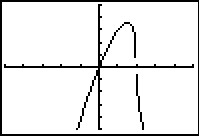
\includegraphics[width=1.5in]{./FurtherGraphics/Algebraic01.jpg}

&

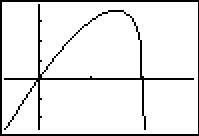
\includegraphics[width=1.5in]{./FurtherGraphics/Algebraic02.jpg} \\

& $y=f(x)$ & $y=f(x)$ near $x=2$.

\end{tabular}

\item In $g(x) = \sqrt{2-\sqrt[4]{x+3}}$, we have two radicals both of which are even indexed.  To satisfy $\sqrt[4]{x+3}$, we require $x+3 \geq 0$ or $x \geq -3$.  To satisfy $ \sqrt{2-\sqrt[4]{x+3}}$, we need $2-\sqrt[4]{x+3} \geq 0$.  While it may be tempting to write this as $2 \geq \sqrt[4]{x+3}$ and take both sides to the fourth power, there are times when this technique will produce erroneous results.\footnote{For instance, $-2 \geq \sqrt[4]{x+3}$, which has no solution or  $-2 \leq \sqrt[4]{x+3}$ whose solution is $[-3,\infty)$.}  Instead, we solve $2-\sqrt[4]{x+3} \geq 0$ using a sign diagram.  If we let $r(x) = 2-\sqrt[4]{x+3}$, we know $x \geq -3$, so we  concern ourselves with only this portion of the number line.  To find the zeros of $r$ we set $r(x) =0$ and solve  $2-\sqrt[4]{x+3}=0$.  We get $\sqrt[4]{x+3} = 2$ so that $\left(\sqrt[4]{x+3}\right)^4 = 2^4$ from which we obtain $x+3 = 16$ or $x=13$.  Since we raised both sides of an equation to an even power, we need to check to see if $x=13$ is an extraneous solution.\footnote{Recall, this means we have produced a candidate which doesn't satisfy the original equation.  Do you remember how raising both sides of an equation to an even power could cause this?}  We find $x=13$ does check since $2-\sqrt[4]{x+3} = 2 - \sqrt[4]{13+3} = 2 - \sqrt[4]{16} = 2 - 2 = 0$. Below is our sign diagram for $r$.



\begin{center}

\begin{mfpic}[10]{0}{8}{-2}{2}

\arrow \polyline{(0,0), (8,0)}

\xmarks{0,4}

\tlabel[cc](0,-1){$-3 \hspace{7pt}$}

\tlabel[cc](2,1){$(+)$}

\tlabel[cc](4,-1){$13$}

\tlabel[cc](4,1){$0$}

\tlabel[cc](6,1){$(-)$}

\end{mfpic}

\end{center}

We find $2-\sqrt[4]{x+3} \geq 0$ on $[-3,13]$ so this is the domain of $g$.  To find a sign diagram for $g$, we look for the zeros of $g$.  Setting $g(x) = 0$ is equivalent to $\sqrt{2-\sqrt[4]{x+3}}=0$.  After squaring both sides, we get $2-\sqrt[4]{x+3} = 0$, whose solution we have found to be $x=13$.   Since we squared both sides, we double check and find $g(13)$ is, in fact, $0$. Our sign diagram and graph of $g$ are below.  Since the domain of $g$ is $[-3,13]$, what we have below is not just a \textit{portion} of the graph of $g$, but the \textit{complete} graph.  It is always above or on the $x$-axis, which verifies our sign diagram.

\begin{tabular}{m{2.5in}c}

\begin{mfpic}[10]{0}{4}{-2}{2}

\polyline{(0,0), (4,0)}

\xmarks{0,4}

\tlabel[cc](0,-1){$-3 \hspace{7pt}$}

\tlabel[cc](2,1){$(+)$}

\tlabel[cc](4,-1){$13$}

\end{mfpic}

&

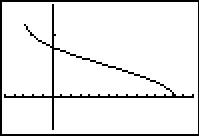
\includegraphics[width=2in]{./FurtherGraphics/Algebraic03.jpg} \\

& The complete graph of $y=g(x)$. \\

\end{tabular}

\item  The radical in $h(x)$ is odd, so our only concern is the denominator.  Setting $x+1=0$ gives $x=-1$, so our domain is $(-\infty, -1) \cup (-1, \infty)$.  To find the zeros of $h$, we set $h(x) = 0$. 
To solve $\sqrt[3]{\frac{8x}{x+1}} = 0$, we cube both sides to get $\frac{8x}{x+1} = 0$.  We get $8x=0$, or $x=0$. Below is the resulting sign diagram and corresponding graph. From the graph, it appears as though $x=-1$ is a vertical asymptote.  Carrying out an analysis as $x \rightarrow -1$ as in Section \ref{RationalGraphs} confirms this.  (We leave the details to the reader.)  Near $x=0$, we have a situation similar to $x=2$ in the graph of $f$ in number 1 above.  Finally, it appears as if the graph of $h$ has a horizontal asymptote $y=2$.  Using techniques from Section \ref{RationalGraphs}, we find as $x \rightarrow \pm \infty$, $\frac{8x}{x+1} \rightarrow 8$.  From this, it is hardly surprising that as $x \rightarrow \pm \infty$, $h(x) = \sqrt[3]{\frac{8x}{x+1}} \approx  \sqrt[3]{8} =2$.

\begin{tabular}{m{2.5in}c}

\begin{mfpic}[10]{-5}{5}{-1}{2}

\arrow \reverse \arrow \polyline{(-5,0),(5,0)}

\xmarks{-2,2}

\tlabel[cc](-3.5,1){$(+)$}

\tlabel[cc](-2,-1){$-1 \hspace{7pt}$}

\tlabel[cc](-2,1){\textinterrobang}

\tlabel[cc](0,1){$(-)$}

\tlabel[cc](2,-1){$0$}

\tlabel[cc](2,1){$0$}

\tlabel[cc](3.5,1){$(+)$}

\end{mfpic}

&

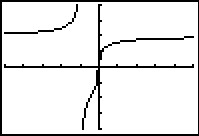
\includegraphics[width=2in]{./FurtherGraphics/Algebraic04.jpg} \\

& $y=h(x)$ \\

\end{tabular}

\item  To find the domain of $k$, we have both an even root and a denominator to concern ourselves with.  To satisfy the square root, $x^2 - 1 \geq 0$.  Setting $r(x) = x^2-1$, we find the zeros of $r$ to be $x = \pm 1$, and we find the sign diagram of $r$ to be


\begin{center}

\begin{mfpic}[10]{-5}{5}{-1}{2}

\arrow \reverse \arrow \polyline{(-5,0),(5,0)}

\xmarks{-2,2}

\tlabel[cc](-3.5,1){$(+)$}

\tlabel[cc](-2,-1){$-1 \hspace{7pt}$}

\tlabel[cc](-2,1){0}

\tlabel[cc](0,1){$(-)$}

\tlabel[cc](2,-1){$1$}

\tlabel[cc](2,1){$0$}

\tlabel[cc](3.5,1){$(+)$}

\end{mfpic}

\end{center}

We find $x^2 - 1 \geq 0$ for $(-\infty, -1] \cup [1, \infty)$.  To keep the denominator of $k(x)$ away from zero, we set $\sqrt{x^2-1} = 0$. We leave it to the reader to verify the solutions are $x = \pm 1$, both of which must be excluded from the domain.    Hence, the domain of $k$ is $(-\infty, -1) \cup (1,\infty)$.  To build the sign diagram for $k$, we need the zeros of $k$.  Setting $k(x) = 0$ results in $\frac{2x}{\sqrt{x^2 - 1}}= 0$.  We get $2x =0$ or $x=0$.  However, $x=0$ isn't in the domain of $k$, which means $k$ has no zeros.  We construct our sign diagram on the domain of $k$ below alongside the graph of $k$. It appears that the graph of $k$ has two vertical asymptotes, one at $x=-1$ and one at $x=1$.   The gap in the graph between the asymptotes is because of the gap in the domain of $k$. Concerning end behavior, there appear to be two horizontal asymptotes, $y = 2$ and $y=-2$.  To see why this is the case, we think of $x\rightarrow \pm \infty$.   The radicand of the denominator $x^2 - 1 \approx x^2$, and as such, $k(x) = \frac{2x}{\sqrt{x^2 - 1}} \approx \frac{2x}{\sqrt{x^2}} = \frac{2x}{|x|}$.  As $x \rightarrow \infty$, we have $|x| = x$ so $k(x) \approx \frac{2x}{x} = 2$.  On the other hand, as $x \rightarrow -\infty$, $|x| = -x$, and as such $k(x) \approx \frac{2x}{-x} = -2$. Finally, it appears as though the graph of $k$ passes the Horizontal Line Test which means $k$ is one to one and $k^{-1}$ exists.  Computing $k^{-1}$ is left as an exercise.

\begin{tabular}{m{2.5in}c}

\begin{mfpic}[10]{-5}{5}{-1}{2}

\arrow  \polyline{(-2,0),(-5,0)}

\arrow  \polyline{(2,0),(5,0)}

\xmarks{-2,2}

\tlabel[cc](-3.5,1){$(-)$}

\tlabel[cc](-2,-1){$-1 \hspace{7pt}$}

\tlabel[cc](-2,1){\textinterrobang}

\tlabel[cc](2,-1){$1$}

\tlabel[cc](2,1){\textinterrobang}

\tlabel[cc](3.5,1){$(+)$}

\end{mfpic}

&

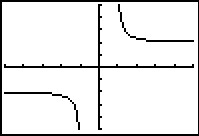
\includegraphics[width=2in]{./FurtherGraphics/Algebraic05.jpg} \\

& $y = k(x)$ \\

\end{tabular}

\qed
\end{enumerate}

\end{ex}

As the previous example illustrates, the graphs of general algebraic functions can have features we've seen before, like vertical and horizontal asymptotes, but they can occur in new and exciting ways. For example, $k(x) = \frac{2x}{\sqrt{x^{2} - 1}}$ had two distinct horizontal asymptotes.  You'll recall that rational functions could have at most one horizontal asymptote.  Also some new characteristics like `unusual steepness'\footnote{The proper Calculus term for this is `vertical tangent', but for now we'll be okay calling it `unusual steepness'.} and cusps\footnote{See page \pageref{cusppicture} for the first reference to this feature.} can appear in the graphs of arbitrary algebraic functions.   Our next example first demonstrates how we can use sign diagrams to solve nonlinear inequalities. (Don't panic.  The technique is very similar to the ones used in Chapters \ref{LinearQuadratic}, \ref{Polynomials} and \ref{Rationals}.)  We then check our answers graphically with a calculator and see some of the new graphical features of the functions in this extended family.

\begin{ex}  Solve the following inequalities.  Check your answers graphically with a calculator.

\begin{multicols}{2}
\begin{enumerate}

\item $x^{2/3} < x^{4/3} - 6$

\item  $3 (2-x)^{1/3} \leq x (2-x)^{-2/3}$

\end{enumerate}
\end{multicols}

{\bf Solution.}  

\begin{enumerate}

\item  To solve $x^{2/3} < x^{4/3} - 6$, we get $0$ on one side and attempt to solve $x^{4/3} - x^{2/3} - 6 > 0$.  We set $r(x) = x^{4/3} - x^{2/3} - 6$ and note that since the denominators in the exponents are $3$, they correspond to cube roots, which means the domain of $r$ is $(-\infty, \infty)$. To find the zeros for the sign diagram, we set $r(x) = 0$ and attempt to solve $x^{4/3} - x^{2/3} - 6 = 0$.  At this point, it may be unclear how to proceed.  We could always try as a last resort converting back to radical notation,  but in this case we can take a cue from Example \ref{usubex}.  Since there are three terms, and the exponent on one of the variable terms, $x^{4/3}$, is exactly twice that of the other, $x^{2/3}$, we have ourselves a `quadratic in disguise' and we can rewrite  $ x^{4/3} - x^{2/3} - 6 = 0$ as $\left(x^{2/3}\right)^2 - x^{2/3} - 6=0$.  If we let $u = x^{2/3}$, then in terms of $u$, we get $u^2 - u - 6 = 0$.  Solving for $u$, we obtain $u = -2$ or $u = 3$.  Replacing $x^{2/3}$ back in for $u$, we get $x^{2/3} = -2$ or $x^{2/3} = 3$.  To avoid the trouble we encountered in the discussion following Definition \ref{rationalexponentdefn}, we now convert back to radical notation.  By interpreting $x^{2/3}$ as $\sqrt[3]{x^2}$ we have $\sqrt[3]{x^2} = -2$ or $\sqrt[3]{x^2}= 3$.  Cubing both sides of these equations results in $x^2 = -8$, which admits no real solution, or $x^2 = 27$, which gives $x = \pm 3 \sqrt{3}$.  We construct a sign diagram and find $x^{4/3} - x^{2/3} - 6 > 0$ on $\left(-\infty, -3 \sqrt{3}\right)\cup \left(3 \sqrt{3}, \infty\right)$.  To check our answer graphically, we set $f(x) = x^{2/3}$ and $g(x) = x^{4/3}-6$.  The solution to  $x^{2/3} < x^{4/3} - 6$ corresponds to the inequality $f(x) < g(x)$, which means we are looking for the $x$ values for which the graph of $f$ is below the graph of $g$.  Using the `Intersect' command we confirm\footnote{Or at least confirm to several decimal places} that the graphs cross at $x= \pm 3\sqrt{3}$.  We see that the graph of $f$ is below the graph of $g$ (the thicker curve) on $\left(-\infty, -3 \sqrt{3}\right)\cup \left(3 \sqrt{3}, \infty\right)$.

\begin{center}

\begin{tabular}{m{2.5in}c}

\begin{mfpic}[10]{-5}{5}{-1}{2}

\arrow \reverse \arrow \polyline{(-5,0),(5,0)}

\xmarks{-2,2}

\tlabel[cc](-3.5,1){$(+)$}

\tlabel[cc](-2,-1){$-3 \sqrt{3} \hspace{7pt}$}

\tlabel[cc](-2,1){$0$}

\tlabel[cc](0,1){$(-)$}

\tlabel[cc](2,-1){$3 \sqrt{3}$}

\tlabel[cc](2,1){$0$}

\tlabel[cc](3.5,1){$(+)$}

\end{mfpic}

&

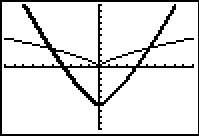
\includegraphics[width=2in]{./FurtherGraphics/Algebraic06.jpg} \\

& $y = f(x)$ and \boldmath $y = g(x)$ \\

\end{tabular}

\end{center}

As a point of interest, if we take a closer look at the graphs of $f$ and $g$  near $x=0$ with the axes off, we see that despite the fact they both involve cube roots, they exhibit different behavior near $x=0$.  The graph of $f$ has a sharp turn, or cusp, while $g$ does not.\footnote{Again, we introduced this feature on page \pageref{cusppicture} as a feature which makes the graph of a function `not smooth'.}

\begin{center}

\begin{tabular}{cc}

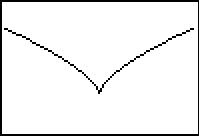
\includegraphics[width=2in]{./FurtherGraphics/Algebraic07.jpg} & 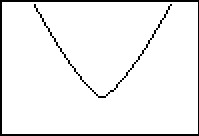
\includegraphics[width=2in]{./FurtherGraphics/Algebraic08.jpg} \\

$y=f(x)$ near $x=0$ & $y=g(x)$ near $x=0$ \\

\end{tabular}

\end{center}

\item  To solve $3 (2-x)^{1/3} \leq x (2-x)^{-2/3}$, we gather all the nonzero terms on one side and obtain $3 (2-x)^{1/3} - x (2-x)^{-2/3} \leq 0$. We set $r(x) = 3 (2-x)^{1/3} - x (2-x)^{-2/3}$.  As in number 1, the denominators of the rational exponents are odd, which means there are no domain concerns there.  However, the negative exponent on the second term indicates a denominator.  Rewriting $r(x)$ with positive exponents, we obtain \[r(x) =  3 (2-x)^{1/3} - \frac{x}{(2-x)^{2/3}}\]  Setting the denominator equal to zero we get $(2-x)^{2/3} = 0$, or $\sqrt[3]{(2-x)^2} = 0$.  After cubing both sides, and subsequently taking square roots, we get $2-x=0$, or $x=2$.  Hence, the domain of $r$ is $(-\infty, 2) \cup (2, \infty)$. To find the zeros of $r$, we set $r(x) = 0$.  There are two school of thought on how to proceed and we demonstrate both.

\begin{itemize}

\item  \textit{Factoring Approach.}  From $r(x) = 3 (2-x)^{1/3} - x (2-x)^{-2/3}$, we note that the quantity $(2-x)$ is common to both terms.  When we factor out common factors, we factor out the quantity with the \textit{smaller} exponent.  In this case, since $-\frac{2}{3} < \frac{1}{3}$, we factor $(2-x)^{-2/3}$ from both quantities.  While it may seem odd to do so, we need to factor $(2-x)^{-2/3}$ \textit{from} $(2-x)^{1/3}$, which results in subtracting the exponent $-\frac{2}{3}$ from $\frac{1}{3}$.  We proceed using the usual properties of exponents.\footnote{And we exercise special care when reducing the $\frac{3}{3}$ power to $1$.}

\[ \begin{array}{rclr}

r(x)  & = & 3 (2-x)^{1/3} - x (2-x)^{-2/3} & \\ [3pt]
      & = & (2-x)^{-2/3} \left[ 3 (2-x)^{\frac{1}{3} - \left(-\frac{2}{3}\right)} - x\right] & \\ [6pt]
      & = & (2-x)^{-2/3}\left[3(2-x)^{3/3} - x\right] & \\ [3pt]
      & = & (2-x)^{-2/3}\left[3(2-x)^{1} - x\right] & \mbox{since $\sqrt[3]{u^3} = \left(\sqrt[3]{u}\right)^{3} = u$} \\ [3pt]
      & = & (2-x)^{-2/3}\left(6-4x\right) & \\ [3pt]
      & = & (2-x)^{-2/3}\left(6-4x\right) & \\
      
\end{array}\]

To solve $r(x) = 0$, we set $(2-x)^{-2/3}\left(6-4x\right) = 0$, or $\frac{6-4x}{(2-x)^{2/3}} = 0$.  We have $6-4x = 0$ or $x = \frac{3}{2}$.

\pagebreak 

\item \textit{Common Denominator Approach.}  We rewrite 

\[ \begin{array}{rclr}

r(x)  & = & 3 (2-x)^{1/3} - x (2-x)^{-2/3} & \\ [3pt]
      & = & 3 (2-x)^{1/3} - \dfrac{x}{(2-x)^{2/3}} & \\ [10pt]
      & = & \dfrac{3 (2-x)^{1/3}(2-x)^{2/3}}{(2-x)^{2/3}} - \dfrac{x}{(2-x)^{2/3}} & \mbox{common denominator} \\ [10pt]
      & = & \dfrac{3 (2-x)^{\frac{1}{3} + \frac{2}{3}}}{(2-x)^{2/3}} - \dfrac{x}{(2-x)^{2/3}} &  \\ [10pt]
      & = & \dfrac{3 (2-x)^{3/3}}{(2-x)^{2/3}} - \dfrac{x}{(2-x)^{2/3}} & \\ [10pt]
      & = & \dfrac{3 (2-x)^1}{(2-x)^{2/3}} - \dfrac{x}{(2-x)^{2/3}} & \mbox{since $\sqrt[3]{u^3} = \left(\sqrt[3]{u}\right)^{3} = u$} \\ [10pt]
      & = & \dfrac{3 (2-x) - x}{(2-x)^{2/3}} & \\ [10pt]
      & = & \dfrac{6-4x}{(2-x)^{2/3}} & \\

       
\end{array}\]


As before, when we set $r(x) = 0$ we obtain $x = \frac{3}{2}$.


\end{itemize}

We now create our sign diagram and find  $3 (2-x)^{1/3} - x (2-x)^{-2/3} \leq 0$ on $\left[\frac{3}{2},2\right) \cup (2, \infty)$.  To check this graphically, we set $f(x)=3 (2-x)^{1/3}$ and $g(x) = x (2-x)^{-2/3}$ (the thicker curve). We confirm that the graphs intersect at $x=\frac{3}{2}$ and the graph of $f$ is below the graph of $g$ for $x \geq \frac{3}{2}$, with the exception of $x=2$ where it appears the graph of $g$ has a vertical asymptote. 

\begin{center}

\begin{tabular}{m{2.5in}c}

\begin{mfpic}[10]{-5}{5}{-1}{2}

\arrow \reverse \arrow \polyline{(-5,0),(5,0)}

\xmarks{-2,2}

\tlabel[cc](-3.5,1){$(+)$}

\tlabel[cc](-2,-1.25){$\frac{3}{2}$}

\tlabel[cc](-2,1){$0$}

\tlabel[cc](0,1){$(-)$}

\tlabel[cc](2,-1){$2$}

\tlabel[cc](2,1){\textinterrobang}

\tlabel[cc](3.5,1){$(-)$}

\end{mfpic}

&

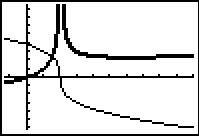
\includegraphics[width=2in]{./FurtherGraphics/Algebraic09.jpg} \\

& $y = f(x)$ and \boldmath $y = g(x)$ \\

\end{tabular}

\end{center}

\end{enumerate}

\vspace{-.30in} \qed

\end{ex}

One application of algebraic functions was given in Example \ref{distancefunctionex} in Section \ref{CartesianPlane}.  Our last example is a more sophisticated application of distance.

\begin{ex} \label{SasquatchCable} Carl wishes to get high speed internet service installed in his remote Sasquatch observation post located $30$ miles from Route $117$. The nearest junction box is located $50$ miles downroad from the post, as indicated in the diagram below.  Suppose it costs $\$ 15$ per mile to run cable along the road and $\$ 20$ per mile to run cable off of the road.

\begin{center}
\begin{mfpic}[15]{-1}{15}{-1}{9}

\xmarks{0, 4}

\arrow \reverse \arrow \polyline{(0,8.75),(0,0.25)}

\arrow \reverse \arrow \polyline{(0.25,0),(3.75,0)}

\arrow \reverse \arrow \polyline{(4.25,0),(9.75,0)}

\arrow \reverse \arrow \polyline{(0,-1),(10,-1)}

\dashed \polyline{(4,0),(0,9)}

\point[3pt]{(0,9), (10,0)}

\tlabel[cc](1.25,9){\scriptsize Outpost}

\tlabel[cc](12,0){\scriptsize Junction Box}

\tlabel[cc](7,0.5){$x$}

\tlabel[cc](2,0.5){$y$}

\tlabel[cc](3,4.5){$z$}

\tlabel[cc](5,-.5){\scriptsize Route $117$}

\tlabel[cc](5,-2){\scriptsize $50$ miles}

\tlabel[cc](-0.5,0){\rotatebox{90}{\hspace{1.5in} \scriptsize $30$ miles}}

\end{mfpic}
\end{center}

\begin{enumerate}

\item  Express the total cost $C$ of connecting the Junction Box to the Outpost as a function of $x$, the number of miles the cable is run along Route $117$ before heading off road directly towards the Outpost.  Determine a reasonable applied domain for the problem.

\item  Use your calculator to graph $y=C(x)$ on its domain.  What is the minimum cost?  How far along Route $117$ should the cable be run before turning off of the road?

\end{enumerate}

{\bf Solution.}

\begin{enumerate}

\item  The cost is broken into two parts:  the cost to run cable along Route $117$ at $\$15$ per mile, and the cost to run it off road at $\$20$ per mile.  Since $x$ represents the miles of cable run along Route $117$, the cost  for that portion is $15x$.  From the diagram, we see that the number of miles the cable is run off road is $z$, so the cost of that portion is $20z$.  Hence, the total cost is $C = 15x + 20z$.  Our next goal is to determine $z$ as a function of $x$.  The diagram suggests we can use the Pythagorean Theorem to get $y^2+30^2 = z^2$.  But we also see $x+y = 50$ so that $y=50-x$.  Hence, $z^2 = (50-x)^2+900$.  Solving for $z$, we obtain $z = \pm \sqrt{(50-x)^2+900}$.  Since $z$ represents a distance, we choose $z = \sqrt{(50-x)^2+900}$ so that our cost as a function of $x$ only is given by \[C(x) = 15x + 20\sqrt{(50-x)^2+900}\] From the context of the problem, we have $0 \leq x \leq 50$.

\item  Graphing $y=C(x)$ on a calculator and using the `Minimum' feature, we find the relative minimum (which is also the absolute minimum in this case) to two decimal places to be $(15.98, 1146.86)$.  Here the $x$-coordinate tells us that in order to minimize cost, we should run $15.98$ miles of cable along Route 117 and then turn off of the road and head towards the outpost. The $y$-coordinate tells us that the minimum cost, in dollars, to do so is $\$1146.86$.  The ability to stream live SasquatchCasts?  Priceless. \qed

\end{enumerate}

\end{ex}

\newpage

\subsection{Exercises}

For each function in Exercises \ref{algfcngraphexfirst} - \ref{algfcngraphexlast} below 

\begin{itemize}

\item Find its domain.
\item Create a sign diagram.
\item Use your calculator to help you sketch its graph and identify any vertical or horizontal asymptotes, `unusual steepness' or cusps.

\end{itemize}

\begin{multicols}{2}
\begin{enumerate}

\item $f(x) = \sqrt{1 - x^{2}}$ \label{algfcngraphexfirst}
\item $f(x) = \sqrt{x^2-1}$

\setcounter{HW}{\value{enumi}}
\end{enumerate}
\end{multicols}

\begin{multicols}{2}
\begin{enumerate}
\setcounter{enumi}{\value{HW}}

\item $f(x) = x \sqrt{1-x^2}$
\item $f(x) = x \sqrt{x^2-1}$

\setcounter{HW}{\value{enumi}}
\end{enumerate}
\end{multicols}

\begin{multicols}{2}
\begin{enumerate}
\setcounter{enumi}{\value{HW}}

\item $f(x) = \sqrt[4]{\dfrac{16x}{x^{2} - 9}}$
\item $f(x) = \dfrac{5x}{\sqrt[3]{x^{3} + 8}}$
\setcounter{HW}{\value{enumi}}
\end{enumerate}
\end{multicols}

\begin{multicols}{2}
\begin{enumerate}
\setcounter{enumi}{\value{HW}}

\item $f(x) = x^{\frac{2}{3}}(x - 7)^{\frac{1}{3}}$
\item $f(x) = x^{\frac{3}{2}}(x - 7)^{\frac{1}{3}}$


\setcounter{HW}{\value{enumi}}
\end{enumerate}
\end{multicols}

\begin{multicols}{2}
\begin{enumerate}
\setcounter{enumi}{\value{HW}}

\item $f(x) = \sqrt{x(x + 5)(x - 4)}$
\item $f(x) = \sqrt[3]{x^{3} + 3x^{2} - 6x - 8}$ \label{algfcngraphexlast}

\setcounter{HW}{\value{enumi}}
\end{enumerate}
\end{multicols}


In Exercises \ref{radicalgraphexfirst} - \ref{radicalgraphexlast}, sketch the graph of $y=g(x)$ by starting with the graph of $y = f(x)$ and using the transformations presented in Section \ref{Transformations}. 

\begin{multicols}{2}
\begin{enumerate}
\setcounter{enumi}{\value{HW}}

\item $f(x) = \sqrt[3]{x}$, $g(x) = \sqrt[3]{x-1}-2$ \label{radicalgraphexfirst}
\item $f(x) = \sqrt[3]{x}$, $g(x) = -2\sqrt[3]{x + 1} + 4$ 

\setcounter{HW}{\value{enumi}}
\end{enumerate}
\end{multicols}

\begin{multicols}{2}
\begin{enumerate}
\setcounter{enumi}{\value{HW}}

\item $f(x) = \sqrt[4]{x}$, $g(x) = \sqrt[4]{x-1}-2$
\item $f(x) = \sqrt[4]{x}$, $g(x) = 3\sqrt[4]{x - 7} - 1$

\setcounter{HW}{\value{enumi}}
\end{enumerate}
\end{multicols}

\begin{multicols}{2}
\begin{enumerate}
\setcounter{enumi}{\value{HW}}

\item $f(x) = \sqrt[5]{x}$, $g(x) = \sqrt[5]{x + 2} + 3$
\item $f(x) = \sqrt[8]{x}$, $g(x) = \sqrt[8]{-x} - 2$ \label{radicalgraphexlast}
\setcounter{HW}{\value{enumi}}
\end{enumerate}

\end{multicols}

\phantomsection
\label{furtherequineqexercises}
In Exercises \ref{algineqexfirst} - \ref{algineqexlast}, solve the equation or inequality.  


\begin{multicols}{2}
\begin{enumerate}
\setcounter{enumi}{\value{HW}}

\item $x+1 = \sqrt{3x+7}$ \label{algineqexfirst}
\item  $2x+1 = \sqrt{3-3x}$

\setcounter{HW}{\value{enumi}}
\end{enumerate}
\end{multicols}

\begin{multicols}{2}
\begin{enumerate}
\setcounter{enumi}{\value{HW}}


\item  $x + \sqrt{3x+10} = -2$
\item  $3x+\sqrt{6-9x}=2$

\setcounter{HW}{\value{enumi}}
\end{enumerate}
\end{multicols}

\begin{multicols}{2}
\begin{enumerate}
\setcounter{enumi}{\value{HW}}


\item $2x - 1 = \sqrt{x + 3}$
\item $x^{\frac{3}{2}} = 8$

\setcounter{HW}{\value{enumi}}
\end{enumerate}
\end{multicols}

\begin{multicols}{2}
\begin{enumerate}
\setcounter{enumi}{\value{HW}}

\item $x^{\frac{2}{3}} = 4$
\item $\sqrt{x - 2} + \sqrt{x - 5} = 3$

\setcounter{HW}{\value{enumi}}
\end{enumerate}
\end{multicols}

\begin{multicols}{2}
\begin{enumerate}
\setcounter{enumi}{\value{HW}}

\item $\sqrt{2x+1} = 3 + \sqrt{4-x}$
\item  $5 - (4-2x)^{\frac{2}{3}} = 1$

\setcounter{HW}{\value{enumi}}
\end{enumerate}
\end{multicols}

\begin{multicols}{2}
\begin{enumerate}
\setcounter{enumi}{\value{HW}}


\item  $10-\sqrt{x-2} \leq 11$
\item $\sqrt[3]{x} \leq x$

\setcounter{HW}{\value{enumi}}
\end{enumerate}
\end{multicols}

\begin{multicols}{2}
\begin{enumerate}
\setcounter{enumi}{\value{HW}}


\item  $2 (x-2)^{-\frac{1}{3}} -\frac{2}{3} x(x-2)^{-\frac{4}{3}} \leq 0$
\item  $-\frac{4}{3} (x-2)^{-\frac{4}{3}} + \frac{8}{9} x (x-2)^{-\frac{7}{3}} \geq 0$

\setcounter{HW}{\value{enumi}}
\end{enumerate}
\end{multicols}

\begin{multicols}{2}
\begin{enumerate}
\setcounter{enumi}{\value{HW}}


\item  $2x^{-\frac{1}{3}}(x-3)^{\frac{1}{3}} + x^{\frac{2}{3}} (x-3)^{-\frac{2}{3}} \geq 0$
\item $\sqrt[3]{x^{3} + 3x^{2} - 6x - 8} > x + 1$


\setcounter{HW}{\value{enumi}}
\end{enumerate}
\end{multicols}

\begin{enumerate}
\setcounter{enumi}{\value{HW}}

\item $\frac{1}{3}x^{\frac{3}{4}}(x - 3)^{-\frac{2}{3}} + \frac{3}{4}x^{-\frac{1}{4}}(x - 3)^{\frac{1}{3}} < 0$
\item $x^{-\frac{1}{3}} (x-3)^{-\frac{2}{3}} - x^{-\frac{4}{3}} (x-3)^{-\frac{5}{3}} (x^2-3x+2) \geq 0$ 
\item $\frac{2}{3}(x + 4)^{\frac{3}{5}}(x - 2)^{-\frac{1}{3}} + \frac{3}{5}(x + 4)^{-\frac{2}{5}}(x - 2)^{\frac{2}{3}} \geq 0$ \label{algineqexlast}



\setcounter{HW}{\value{enumi}}
\end{enumerate}

\begin{enumerate}
\setcounter{enumi}{\value{HW}}

\item  Rework Example \ref{SasquatchCable} so that the outpost is 10 miles from Route 117 and the nearest junction box is 30 miles down the road for the post.


\item  The volume $V$ of a right cylindrical cone depends on the radius of its base $r$ and its height $h$ and is given by the formula $V = \frac{1}{3} \pi r^2 h$.  The surface area $S$ of a right cylindrical cone also depends on $r$ and $h$ according to the formula $S = \pi r \sqrt{r^2+h^2}$.  Suppose a cone is to have a volume of 100 cubic centimeters. 

\begin{enumerate}

\item  \label{heightintermsofr} Use the formula for volume to find the height $h$ as a function of $r$.
\item  Use the formula for surface area and your answer to \ref{heightintermsofr} to find the surface area $S$ as a function of $r$.
\item  Use your calculator to find the values of $r$ and $h$ which minimize the surface area.  What is the minimum surface area?  Round your answers to two decimal places.

\end{enumerate}

\item \label{WindChillTemperature} The \href{http://www.nws.noaa.gov/om/windchill/windchillglossary.shtml}{\underline{National Weather Service}} uses the following formula to calculate the wind chill: \[ W = 35.74 + 0.6215 \, T_{a} - 35.75\, V^{0.16} + 0.4275 \, T_{a} \, V^{0.16}  \] where $W$ is the wind chill temperature in $^{\circ}$F, $T_{a}$ is the air temperature in $^{\circ}$F, and  $V$ is the wind speed in miles per hour.  Note that $W$ is defined only for air temperatures at or lower than $50^{\circ}$F and wind speeds above $3$ miles per hour.

\begin{enumerate}

\item  Suppose the air temperature is $42^{\circ}$ and the wind speed is $7$ miles per hour. Find the wind chill temperature.  Round your answer to two decimal places.

\item  Suppose the air temperature is $37^{\circ}$F and the wind chill temperature is $30^{\circ}$F.  Find the wind speed.  Round your answer to two decimal places. 

\end{enumerate}

\item  As a follow-up to Exercise \ref{WindChillTemperature}, suppose the air temperature is $28^{\circ}$F.  

\begin{enumerate}

\item Use the formula from Exercise \ref{WindChillTemperature} to find an expression for the wind chill temperature as a function of the wind speed, $W(V)$.  

\item  \label{WindChill0} Solve $W(V) = 0$, round your answer to two decimal places,  and interpret.  

\item  Graph the function $W$ using your calculator and check your answer to part \ref{WindChill0}. 


\end{enumerate}

\item \label{pendulumproblem} The period of a pendulum in seconds is given by \[T = 2\pi \sqrt{\dfrac{L}{g}}\](for small displacements) where $L$ is the length of the pendulum in meters and $g = 9.8$ meters per second per second is the acceleration due to gravity.  My Seth-Thomas antique schoolhouse clock needs $T = \frac{1}{2}$ second and I can adjust the length of the pendulum via a small dial on the bottom of the bob.  At what length should I set the pendulum?


\item The Cobb-Douglas production model states that the yearly total dollar value of the production output $P$ in an economy is a function of labor $x$ (the total number of hours worked in a year) and capital $y$ (the total dollar value of all of the stuff purchased in order to make things).  Specifically, $P = ax^{b}y^{1 - b}$.  By fixing $P$, we create what's known as an `isoquant' and we can then solve for $y$ as a function of $x$.  Let's assume that the Cobb-Douglas production model for the country of Sasquatchia is $P = 1.23x^{0.4}y^{0.6}$.  

\begin{enumerate}

\item Let $P = 300$ and solve for $y$ in terms of $x$.  If $x = 100$, what is $y$?

\item Graph the isoquant $300 = 1.23x^{0.4}y^{0.6}$.  What information does an ordered pair $(x, y)$ which makes $P = 300$ give you?  With the help of your classmates, find several different combinations of labor and capital all of which yield $P = 300$.  Discuss any patterns you may see.

\end{enumerate}




\item According to Einstein's Theory of Special Relativity, the observed mass $m$ of an object is a function of how fast the object is traveling.  Specifically, \[m(x) = \dfrac{m_{r}}{\sqrt{1 - \dfrac{x^{2}}{c^{2}}}}\] where $m(0)=m_{r}$ is the mass of the object at rest, $x$ is the speed of the object and $c$ is the speed of light. 

\begin{enumerate}

\item Find the applied domain of the function.

\item Compute $m(.1c), \, m(.5c), \, m(.9c)$ and $m(.999c)$.

\item As $x \rightarrow c^{-}$, what happens to $m(x)$?

\item How slowly must the object be traveling so that the observed mass is no greater than 100 times its mass at rest?

\end{enumerate}


\item Find the inverse of $k(x) = \dfrac{2x}{\sqrt{x^{2} - 1}}$.

\pagebreak

\item \label{pursuitfurther} Suppose Fritzy the Fox, positioned at a point $(x,y)$ in the first quadrant, spots Chewbacca the Bunny at $(0,0)$.   Chewbacca begins to run along a fence (the positive $y$-axis) towards his warren.  Fritzy, of course, takes chase and constantly adjusts his direction so that he is always running directly at Chewbacca.  If Chewbacca's speed is $v_{\mbox{\tiny$1$}}$ and  Fritzy's speed is $v_{\mbox{\tiny$2$}}$, the path Fritzy will take to intercept Chewbacca, provided $v_{\mbox{\tiny$2$}}$ is directly proportional to, but not equal to, $v_{\mbox{\tiny$1$}}$ is modeled by

\[ y = \dfrac{1}{2} \left(\dfrac{x^{1+ v_{1}/v_{2}}}{1+v_{\mbox{\tiny$1$}}/v_{\mbox{\tiny$2$}}}- \dfrac{x^{1-v_{\mbox{\tiny$1$}}/v_{\mbox{\tiny$2$}}}}{1-v_{\mbox{\tiny$1$}}/v_{\mbox{\tiny$2$}}}\right) + \dfrac{v_{\mbox{\tiny$1$}} v_{\mbox{\tiny$2$}}}{v_{\mbox{\tiny$2$}}^2-v_{\mbox{\tiny$1$}}^2} \]

\begin{enumerate}

\item  Determine the path that Fritzy will take if he runs exactly twice as fast as Chewbacca;  that is, $v_{\mbox{\tiny$2$}} = 2v_{\mbox{\tiny$1$}}$. Use your calculator to graph this path for $x \geq 0$.  What is the significance of the $y$-intercept of the graph?

\item  Determine the path Fritzy will take if Chewbacca runs exactly twice as fast as he does;  that is, $v_{\mbox{\tiny$1$}} = 2v_{\mbox{\tiny$2$}}$.  Use your calculator to graph this path for $x > 0$.  Describe the behavior of $y$ as $x \rightarrow 0^{+}$ and interpret this physically.

\item  With the help of your classmates, generalize parts (a) and (b) to two cases:  $v_{\mbox{\tiny$2$}} > v_{\mbox{\tiny$1$}}$ and $v_{\mbox{\tiny$2$}} < v_{\mbox{\tiny$1$}}$.   We will discuss the case of $v_{\mbox{\tiny$1$}} = v_{\mbox{\tiny$2$}}$ in Exercise \ref{pursuitlog} in Section \ref{ExpLogApplications}.

\end{enumerate}



\item Verify the Quotient Rule for Radicals in Theorem \ref{radicalprops}.

\item Show that $\left(x^{\frac{3}{2}}\right)^{\frac{2}{3}} = x$ for all $x \geq 0$.

\item Show that $\sqrt[3]{2}$ is an irrational number by first showing that it is a zero of $p(x) = x^{3} - 2$ and then showing $p$ has no rational zeros.  (You'll need the Rational Zeros Theorem, Theorem \ref{RZT}, in order to show this last part.) \label{nthrootsareirrational}

\item With the help of your classmates, generalize Exercise \ref{nthrootsareirrational} to show that $\sqrt[n]{c}$ is an irrational number for any natural numbers $c \geq 2$ and $n \geq 2$ provided that $c \neq p^{n}$ for some natural number $p$.

\end{enumerate}

\newpage

\subsection{Answers}

\begin{enumerate}

\item \begin{multicols}{2}
$f(x) = \sqrt{1 - x^2}$\\
Domain: $[-1, 1]$\\
\begin{mfpic}[20][10]{0}{4}{-1.5}{1.5}
\polyline{(0,0), (4,0)}
\xmarks{0,4}
\tlabel[cc](0,-1){$-1 \hspace{7pt}$}
\tlabel[cc](2,1){$(+)$}
\tlabel[cc](0,1){$0$}
\tlabel[cc](4,1){$0$}
\tlabel[cc](4,-1){$1$}
\end{mfpic}

No asymptotes\\
Unusual steepness at $x = -1$ and $x = 1$\\
No cusps\\

\vfill

\columnbreak

\begin{mfpic}[50]{-1.5}{1.5}{-0.15}{1.5}
\point[3pt]{(0,1), (-1,0), (1,0)}
\parafcn{0,3.14159,0.1}{(cos(t),sin(t))}
\axes
\tlabel[cc](1.5,-0.15){\scriptsize $x$}
\tlabel[cc](0.25,1.5){\scriptsize $y$}
\xmarks{-1,1}
\ymarks{1}
\tlpointsep{4pt}
\scriptsize
\axislabels {x}{{$-1 \hspace{6pt}$} -1, {$1$} 1}
\axislabels {y}{{$1$} 1}
\normalsize
\end{mfpic}

\end{multicols}


\item \begin{multicols}{2}
$f(x) = \sqrt{x^2-1}$\\
Domain: $(-\infty, -1] \cup [1,\infty)$\\
\begin{mfpic}[20][10]{0}{4}{-1.5}{1.5}
\arrow \polyline{(2,0), (0,0)}
\arrow \polyline{(3,0), (5,0)}
\xmarks{2,3}
\tlabel[cc](2,-1){$-1 \hspace{7pt}$}
\tlabel[cc](1,1){$(+)$}
\tlabel[cc](4,1){$(+)$}
\tlabel[cc](2,1){$0$}
\tlabel[cc](3,1){$0$}
\tlabel[cc](3,-1){$1$}
\end{mfpic}

No asymptotes\\
Unusual steepness at $x = -1$ and $x = 1$\\
No cusps\\

\vfill

\columnbreak


\begin{mfpic}[20]{-4}{4}{-1}{4}
\point[3pt]{(-1,0), (1,0)}
\arrow \parafcn{0,2,0.1}{(cosh(t),sinh(t))}
\arrow \parafcn{0,2,0.1}{(-cosh(t),sinh(t))}
\axes
\tlabel[cc](4,-0.25){\scriptsize $x$}
\tlabel[cc](0.25,4){\scriptsize $y$}
\xmarks{-3,-2,-1,1,2,3}
\ymarks{1,2,3}
\tlpointsep{4pt}
\scriptsize
\axislabels {x}{{$-3 \hspace{6pt}$} -3,{$-2 \hspace{6pt}$} -2,{$-1 \hspace{6pt}$} -1, {$1$} 1, {$2$} 2, {$3$} 3}
\axislabels {y}{{$1$} 1, {$2$} 2, {$3$} 3}
\normalsize
\end{mfpic}


\end{multicols}

\item \begin{multicols}{2}
$f(x) = x\sqrt{1-x^2}$\\
Domain: $[-1,1]$\\
\begin{mfpic}[20][10]{0}{4}{-1.5}{1.5}
\polyline{(0,0), (5,0)}
\xmarks{0,2.5,5}
\tlabel[cc](0,-1){$-1 \hspace{7pt}$}
\tlabel[cc](0,1){$0$}
\tlabel[cc](1.25,1){$(-)$}
\tlabel[cc](2.5,-1){$0$}
\tlabel[cc](3.75,1){$(+)$}
\tlabel[cc](2.5,1){$0$}
\tlabel[cc](5,-1){$1$}
\tlabel[cc](5,1){$0$}
\end{mfpic}

No asymptotes\\
Unusual steepness at $x = -1$ and $x = 1$\\
No cusps\\

\vfill

\columnbreak

\begin{mfpic}[50][40]{-1.5}{1.5}{-1}{1.5}
\point[3pt]{(-1,0), (1,0),(0,0)}
\parafcn{0,3.14159,0.1}{(cos(t),cos(t)*sin(t))}
\axes
\tlabel[cc](1.5,-0.15){\scriptsize $x$}
\tlabel[cc](0.25,1.5){\scriptsize $y$}
\xmarks{-1,1}
\ymarks{-1,1}
\tlpointsep{4pt}
\scriptsize
\axislabels {x}{{$-1 \hspace{6pt}$} -1, {$1$} 1}
\axislabels {y}{{$1$} 1,{$-1$} -1}
\normalsize
\end{mfpic}


\end{multicols}

\item \begin{multicols}{2}
$f(x) = x\sqrt{x^2-1}$\\
Domain: $(-\infty, -1] \cup [1,\infty)$\\
\begin{mfpic}[20][10]{0}{4}{-1.5}{1.5}
\arrow \polyline{(2,0), (0,0)}
\arrow \polyline{(3,0), (5,0)}
\xmarks{2,3}
\tlabel[cc](2,-1){$-1 \hspace{7pt}$}
\tlabel[cc](1,1){$(-)$}
\tlabel[cc](4,1){$(+)$}
\tlabel[cc](2,1){$0$}
\tlabel[cc](3,1){$0$}
\tlabel[cc](3,-1){$1$}
\end{mfpic}

No asymptotes\\
Unusual steepness at $x = -1$ and $x = 1$\\
No cusps\\

\vfill

\columnbreak


\begin{mfpic}[20][15]{-4}{4}{-4}{4}
\point[3pt]{(-1,0), (1,0)}
\arrow \parafcn{0,2,0.1}{(cosh(t),sinh(t))}
\arrow \parafcn{0,2,0.1}{(-cosh(t),-sinh(t))}
\axes
\tlabel[cc](4,-0.25){\scriptsize $x$}
\tlabel[cc](0.25,4){\scriptsize $y$}
\xmarks{-3,-2,-1,1,2,3}
\ymarks{-3,-2,-1,1,2,3}
\tlpointsep{4pt}
\scriptsize
\axislabels {x}{{$-3 \hspace{6pt}$} -3,{$-2 \hspace{6pt}$} -2,{$-1 \hspace{6pt}$} -1, {$1$} 1, {$2$} 2, {$3$} 3}
\axislabels {y}{{$-3$} -3,{$-2$} -2,{$-1$} -1,{$1$} 1, {$2$} 2, {$3$} 3}
\normalsize
\end{mfpic}


\end{multicols}

\pagebreak

\item \begin{multicols}{2} 
$f(x) = \sqrt[4]{\dfrac{16x}{x^2 - 9}}$\\
Domain: $(-3, 0] \cup (3, \infty)$\\
\begin{mfpic}[15]{-3}{6}{-1}{1}
\polyline{(-3,0),(0,0)}
\arrow  \polyline{(3,0),(6,0)}
\xmarks{-3,0,3}
\tlabel[cc](-1.5,0.75){$(+)$}
\tlabel[cc](-3,-0.75){$-3 \hspace{7pt}$}
\tlabel[cc](-3,0.75){\textinterrobang}
\tlabel[cc](0,-0.75){$0$}
\tlabel[cc](0,0.75){$0$}
\tlabel[cc](3,0.75){\textinterrobang}
\tlabel[cc](3,-0.75){$3$}
\tlabel[cc](4.5,0.75){$(+)$}
\end{mfpic}

Vertical asymptotes: $x = -3$ and $x = 3$\\
Horizontal asymptote: $y = 0$\\
Unusual steepness at $x = 0$\\
No cusps\\


\vfill

\columnbreak

\begin{mfpic}[15]{-3.5}{9}{-1}{6}
\point[3pt]{(0,0)}
\dashed \polyline{(-3,-1), (-3,6)}
\dashed \polyline{(3,-1), (3,6)}
\arrow \reverse \function{-2.93,0,0.1}{((16*x)/((x**2) - 9))**(0.25)}
\arrow \reverse \arrow \function{3.05,9,0.1}{((16*x)/((x**2) - 9))**(0.25)}
\axes
\tlabel[cc](9,-0.5){\scriptsize $x$}
\tlabel[cc](0.5,6){\scriptsize $y$}
\xmarks{-3 step 1 until 8}
\ymarks{1,2,3,4,5}
\tlpointsep{4pt}
\scriptsize
\axislabels {x}{{$-3 \hspace{6pt}$} -3, {$-2 \hspace{6pt}$} -2, {$-1 \hspace{6pt}$} -1, {$1$} 1, {$2$} 2, {$3$} 3, {$4$} 4, {$5$} 5, {$6$} 6, {$7$} 7, {$8$} 8}
\axislabels {y}{{$1$} 1, {$2$} 2, {$3$} 3, {$4$} 4, {$5$} 5}
\normalsize
\end{mfpic}

\end{multicols}

\item \begin{multicols}{2} 
$f(x) = \dfrac{5x}{\sqrt[3]{x^{3} + 8}}$\\
Domain: $(-\infty, -2) \cup (-2, \infty)$\\
\begin{mfpic}[20]{-4}{2}{-1}{1}
\arrow \reverse \arrow \polyline{(-4,0),(2,0)}
\xmarks{-2,0}
\tlabel[cc](-3, 0.5){$(+)$}
\tlabel[cc](-2,-0.5){$-2 \hspace{7pt}$}
\tlabel[cc](-2,0.5){\textinterrobang}
\tlabel[cc](-1,0.5){$(-)$}
\tlabel[cc](0,-0.5){$0$}
\tlabel[cc](0,0.5){$0$}
\tlabel[cc](1,0.5){$(+)$}
\end{mfpic}

Vertical asymptote $x = -2$\\
Horizontal asymptote $y = 5$\\
No unusual steepness or cusps\\

\vfill

\columnbreak

\begin{mfpic}[10][8]{-5}{5}{-7}{9}
\point[3pt]{(0,0)}
\dashed \polyline{(-5,5), (5,5)}
\dashed \polyline{(-2,-7), (-2,9)}
\arrow \reverse \arrow \function{-5,-2.2,0.1}{(-5*x)/((-(x**3) - 8)**(1/3))}
\arrow \reverse \arrow \function{-1.8,5,0.1}{(5*x)/(((x**3) + 8)**(1/3))}
\axes
\tlabel[cc](5,-0.5){\scriptsize $x$}
\tlabel[cc](0.5,9){\scriptsize $y$}
\xmarks{-4 step 1 until 4}
\ymarks{-6 step 1 until 8}
\tlpointsep{4pt}
\tiny
\axislabels {x}{{$-4 \hspace{6pt}$} -4, {$-3 \hspace{6pt}$} -3, {$-2 \hspace{6pt}$} -2, {$-1 \hspace{6pt}$} -1, {$1$} 1, {$2$} 2, {$3$} 3, {$4$} 4}
\axislabels {y}{{$-6$} -6, {$-5$} -5, {$-4$} -4, {$-3$} -3, {$-2$} -2, {$-1$} -1, {$1$} 1, {$2$} 2, {$3$} 3, {$4$} 4, {$5$} 5, {$6$} 6, {$7$} 7, {$8$} 8}
\normalsize
\end{mfpic}

\end{multicols}

\item \begin{multicols}{2} 
$f(x) = x^{\frac{2}{3}}(x - 7)^{\frac{1}{3}}$\\
Domain: $(-\infty, \infty)$\\
\begin{mfpic}[10]{-3}{10}{-2}{2}
\arrow \reverse \arrow \polyline{(-3,0),(10,0)}
\xmarks{0,7}
\tlabel[cc](-1.5,1){$(-)$}
\tlabel[cc](0,-1){$0$}
\tlabel[cc](0,1){$0$}
\tlabel[cc](3.5,1){$(-)$}
\tlabel[cc](7,-1){$7$}
\tlabel[cc](7,1){$0$}
\tlabel[cc](8.5,1){$(+)$}
\end{mfpic}

No vertical or horizontal asymptotes\footnote{Using Calculus it can be shown that $y = x - \frac{7}{3}$ is a slant asymptote of this graph.}\\
Unusual steepness at $x = 7$\\
Cusp at $x = 0$\\

\vfill

\columnbreak

\begin{mfpic}[10]{-4}{10}{-5}{5.5}
\point[3pt]{(0,0), (7,0)}
\arrow \reverse \function{-3,0,0.1}{-((x**2)**(1/3))*((7 - x)**(1/3))}
\function{0,7,0.1}{-((x**2)**(1/3))*((7 - x)**(1/3))}
\arrow \function{7,9,0.1}{((x**2)**(1/3))*((x - 7)**(1/3))}
\axes
\tlabel[cc](10,-0.5){\scriptsize $x$}
\tlabel[cc](0.5,5.5){\scriptsize $y$}
\xmarks{-3 step 1 until 9}
\ymarks{-4 step 1 until 5}
\tlpointsep{4pt}
\tiny
\axislabels {x}{{$-3 \hspace{6pt}$} -3, {$-2 \hspace{6pt}$} -2, {$-1 \hspace{6pt}$} -1, {$1$} 1, {$2$} 2, {$3$} 3, {$4$} 4, {$5$} 5, {$6$} 6, {$7$} 7, {$8$} 8, {$9$} 9}
\axislabels {y}{{$-4$} -4, {$-3$} -3, {$-2$} -2, {$-1$} -1, {$1$} 1, {$2$} 2, {$3$} 3, {$4$} 4, {$5$} 5}
\normalsize
\end{mfpic}

\end{multicols}

\item \begin{multicols}{2} 
$f(x) = x^{\frac{3}{2}}(x - 7)^{\frac{1}{3}}$\\
Domain: $[0, \infty)$\\
\begin{mfpic}[15]{0}{10}{-1}{1}
\reverse \arrow \polyline{(0,0),(10,0)}
\xmarks{0, 7}
\tlabel[cc](0,-0.5){$0$}
\tlabel[cc](0,0.5){$0$}
\tlabel[cc](3.5, 0.5){$(-)$}
\tlabel[cc](7,-0.5){$7$}
\tlabel[cc](7,0.5){$0$}
\tlabel[cc](8, 0.5){$(+)$}
\end{mfpic}

No asymptotes\\
Unusual steepness at $x = 7$\\
No cusps\\

\vfill

\columnbreak

\begin{mfpic}[15][3]{-1}{8.5}{-20}{30}
\point[3pt]{(0,0), (7,0)}
\function{0,7,0.1}{-(x**1.5)*((7 - x)**(1/3))}
\arrow \function{7,8.5,0.1}{(x**1.5)*((x - 7)**(1/3))}
\axes
\tlabel[cc](8.5,-3){\scriptsize $x$}
\tlabel[cc](0.5,30){\scriptsize $y$}
\xmarks{1 step 1 until 8}
\ymarks{-15 step 5 until 25}
\tlpointsep{4pt}
\scriptsize
\axislabels {x}{{$1$} 1, {$2$} 2, {$3$} 3, {$4$} 4, {$5$} 5, {$6$} 6, {$7$} 7, {$8$} 8}
\axislabels {y}{{$-15$} -15, {$-10$} -10, {$-5$} -5, {$5$} 5, {$10$} 10, {$15$} 15, {$20$} 20, {$25$} 25}
\normalsize
\end{mfpic}

\end{multicols}

\item \begin{multicols}{2} 
$f(x) = \sqrt{x(x + 5)(x - 4)}$\\
Domain: $[-5, 0] \cup [4, \infty)$\\
\begin{mfpic}[10]{-5}{8}{-1}{1}
\polyline{(-5,0),(0,0)}
\arrow  \polyline{(4,0),(8,0)}
\xmarks{-5,0,4}
\tlabel[cc](-5,-1){$-5 \hspace{7pt}$}
\tlabel[cc](-5,1){$0$}
\tlabel[cc](-2.5,1){$(+)$}
\tlabel[cc](0,-1){$0$}
\tlabel[cc](0,1){$0$}
\tlabel[cc](4,-1){$4$}
\tlabel[cc](4,1){$0$}
\tlabel[cc](6,1){$(+)$}
\end{mfpic}

No asymptotes\\
Unusual steepness at $x = -5, x = 0$ and $x = 4$\\
No cusps\\

\vfill

\columnbreak

\begin{mfpic}[10]{-6}{6}{-1}{10}
\point[3pt]{(-5,0),(0,0),(4,0)}
\function{-5,0,0.1}{sqrt((x**3) + (x**2) - (20*x))}
\arrow \function{4,5.5,0.1}{sqrt((x**3) + (x**2) - (20*x))}
\axes
\tlabel[cc](6,-0.5){\scriptsize $x$}
\tlabel[cc](0.5,10){\scriptsize $y$}
\xmarks{-5 step 1 until 5}
\ymarks{1 step 1 until 9}
\tlpointsep{4pt}
\tiny
\axislabels {x}{{$-5 \hspace{6pt}$} -5, {$-4 \hspace{6pt}$} -4, {$-3 \hspace{6pt}$} -3, {$-2 \hspace{6pt}$} -2, {$-1 \hspace{6pt}$} -1, {$1$} 1, {$2$} 2, {$3$} 3, {$4$} 4, {$5$} 5}
\axislabels {y}{{$1$} 1, {$2$} 2, {$3$} 3, {$4$} 4, {$5$} 5, {$6$} 6, {$7$} 7, {$8$} 8, {$9$} 9}
\normalsize
\end{mfpic}

\end{multicols}

\item \begin{multicols}{2} 
$f(x) = \sqrt[3]{x^{3} + 3x^{2} - 6x - 8}$\\
Domain: $(-\infty, \infty)$\\
\begin{mfpic}[10]{-8}{6}{-1}{1}
\arrow \reverse \arrow \polyline{(-8,0),(6,0)}
\xmarks{-4,-1,2}
\tlabel[cc](-6,1){$(-)$}
\tlabel[cc](-4,-1){$-4 \hspace{7pt}$}
\tlabel[cc](-4,1){$0$}
\tlabel[cc](-2.5,1){$(+)$}
\tlabel[cc](-1,-1){$-1 \hspace{7pt}$}
\tlabel[cc](-1,1){$0$}
\tlabel[cc](0.5,1){$(-)$}
\tlabel[cc](2,-1){$2$}
\tlabel[cc](2,1){$0$}
\tlabel[cc](4,1){$(+)$}
\end{mfpic}

No vertical or horizontal asymptotes\footnote{Using Calculus it can be shown that $y = x + 1$ is a slant asymptote of this graph.}\\
Unusual steepness at $x = -4, x = -1$ and $x = 2$\\
No cusps\\

\vfill

\columnbreak

\begin{mfpic}[10]{-6}{6}{-5}{7}
\point[3pt]{(-4,0),(-1,0),(2,0)}
\arrow \reverse \function{-6,-4,0.1}{-((-((x**3) + (3*(x**2)) - (6*x) - 8))**(1/3))}
\function{-4,-1,0.1}{((x**3) + (3*(x**2)) - (6*x) - 8)**(1/3)}
\function{-1,2,0.1}{-((-((x**3) + (3*(x**2)) - (6*x) - 8))**(1/3))}
\arrow \function{2,6,0.1}{((x**3) + (3*(x**2)) - (6*x) - 8)**(1/3)}
\axes
\tlabel[cc](6,-0.5){\scriptsize $x$}
\tlabel[cc](0.5,7){\scriptsize $y$}
\xmarks{-5 step 1 until 5}
\ymarks{-4 step 1 until 6}
\tlpointsep{4pt}
\tiny
\axislabels {x}{{$-5 \hspace{6pt}$} -5, {$-4 \hspace{6pt}$} -4, {$-3 \hspace{6pt}$} -3, {$-2 \hspace{6pt}$} -2, {$-1 \hspace{6pt}$} -1, {$1$} 1, {$2$} 2, {$3$} 3, {$4$} 4, {$5$} 5}
\axislabels {y}{{$-4$} -4, {$-3$} -3, {$-2$} -2, {$-1$} -1, {$1$} 1, {$2$} 2, {$3$} 3, {$4$} 4, {$5$} 5, {$6$} 6}
\normalsize
\end{mfpic}

\end{multicols}

\setcounter{HW}{\value{enumi}}
\end{enumerate}

\begin{multicols}{2}
\begin{enumerate}
\setcounter{enumi}{\value{HW}}


\item $g(x) = \sqrt[3]{x-1}-2$ \\ 

\begin{mfpic}[8][13]{-10}{12}{-5}{1}
\arrow \reverse \arrow \parafcn{-4.2,0.2,0.1}{(((t + 2)**3) + 1,t)}
\axes
\tlabel[cc](12,-0.5){\scriptsize $x$}
\tlabel[cc](0.75,1){\scriptsize $y$}
\point[3pt]{(-7, -4), (0,-3), (1,-2), (2,-1), (9,0)}
\ymarks{-4,-3,-2,-1}
\xmarks{-9 step 1 until 11}
\tiny
\tlpointsep{4pt}
\axislabels {y}{{$-4$} -4, {$-3$} -3, {$-2$} -2, {$-1$} -1}
\axislabels {x}{{$-9 \hspace{6pt}$} -9, {$-7 \hspace{6pt}$} -7,  {$-5 \hspace{6pt}$} -5,  {$-3 \hspace{6pt}$} -3,  {$-1 \hspace{6pt}$} -1, {$1$} 1,  {$3$} 3, {$5$} 5,  {$7$} 7,  {$9$} 9, {$11$} 11}
\normalsize
\end{mfpic}

\vfill

\columnbreak

\item $g(x) = -2\sqrt[3]{x + 1} + 4$\\

\begin{mfpic}[10][9]{-7}{9}{-1}{8}
\point[3pt]{(-2,6),(-1,4),(0,2),(7,0)}
\arrow \reverse \function{-7,-1,0.1}{2*((-x - 1)**(1/3)) + 4}
\arrow \function{-1,8.5,0.1}{-2*((x + 1)**(1/3)) + 4}
\axes
\tlabel[cc](9,-0.5){\scriptsize $x$}
\tlabel[cc](0.5,8){\scriptsize $y$}
\xmarks{-6 step 1 until 8}
\ymarks{1 step 1 until 7}
\tlpointsep{4pt}
\tiny
\axislabels {x}{ {$-5 \hspace{6pt}$} -5,  {$-3 \hspace{6pt}$} -3, {$-1 \hspace{6pt}$} -1, {$1$} 1,  {$3$} 3,  {$5$} 5,  {$7$} 7 }
\axislabels {y}{{$1$} 1, {$2$} 2, {$3$} 3, {$4$} 4, {$5$} 5, {$6$} 6, {$7$} 7}
\normalsize
\end{mfpic}

\setcounter{HW}{\value{enumi}}
\end{enumerate}
\end{multicols}


\begin{multicols}{2}
\begin{enumerate}
\setcounter{enumi}{\value{HW}}


\item $g(x) = \sqrt[4]{x-1}-2$\\

\begin{mfpic}[8][25]{-1}{22}{-3}{1}
\arrow \parafcn{-2,0.12,0.1}{(((t + 2)**4) + 1,t)}
\axes
\tlabel[cc](22,-0.75){\scriptsize $x$}
\tlabel[cc](0.5,1){\scriptsize $y$}
\point[3pt]{(1,-2),(2,-1),(17,0)}
\ymarks{-2,-1}
\xmarks{1 step 1 until 21}
\tiny
\tlpointsep{4pt}
\axislabels {y}{{$-2$} -2, {$-1$} -1}
\axislabels {x}{{$1$} 1,  {$3$} 3, {$5$} 5, {$7$} 7,  {$9$} 9,  {$11$} 11,  {$13$} 13,  {$15$} 15,  {$17$} 17, {$19$} 19,  {$21$} 21}
\normalsize
\end{mfpic}

\vfill

\columnbreak

\item $g(x) = 3\sqrt[4]{x - 7} - 1$\\

\begin{mfpic}[5][13]{-1}{25}{-2}{6}
\point[3pt]{(7,-1),(8,2),(23,5)}
\arrow \function{7,25,0.1}{3*((x - 7)**(0.25)) - 1}
\axes
\tlabel[cc](25,-0.5){\scriptsize $x$}
\tlabel[cc](0.5,6){\scriptsize $y$}
\xmarks{1 step 1 until 23}
\ymarks{-1 step 1 until 5}
\tlpointsep{4pt}
\tiny
\axislabels {x}{{$7$} 7, {$8$} 8, {$23$} 23}
\axislabels {y}{{$-1$} -1, {$1$} 1, {$2$} 2, {$3$} 3, {$4$} 4, {$5$} 5}
\normalsize
\end{mfpic}

\setcounter{HW}{\value{enumi}}
\end{enumerate}
\end{multicols}

\begin{multicols}{2}
\begin{enumerate}
\setcounter{enumi}{\value{HW}}

\item $g(x) = \sqrt[5]{x + 2} + 3$\\

\begin{mfpic}[2][10]{-37}{33}{-1}{6}
\point[2pt]{(-34,1),(-3,2),(-2,3),(-1,4),(30,5)}
\arrow \function{-2,33,0.1}{((x + 2)**(0.20)) + 3}
\arrow \reverse \function{-37,-2,0.1}{(-((-x - 2)**(0.20))) + 3}
\axes
\tlabel[cc](33,-0.5){\scriptsize $x$}
\tlabel[cc](2,6){\scriptsize $y$}
\xmarks{-34,-2,30}
\ymarks{1 step 1 until 5}
\tlpointsep{4pt}
\tiny
\axislabels {x}{{$-34 \hspace{5pt}$} -34, {$-2 \hspace{5pt}$} -2, {$30$} 30}
\axislabels {y}{{$1$} 1, {$2$} 2, {$3$} 3, {$4$} 4, {$5$} 5}
\normalsize
\end{mfpic}

\item $g(x) = \sqrt[8]{-x} - 2$\\

\begin{mfpic}[3][15]{-45}{5}{-3}{1}
\point[2pt]{(0,-2),(-1,-1)}
\arrow \reverse \function{-45,0,0.1}{((-x)**0.125) - 2}
\axes
\tlabel[cc](5,-0.5){\scriptsize $x$}
\tlabel[cc](1.5,1){\scriptsize $y$}
\xmarks{-40,-30,-20,-10}
\ymarks{-2,-1}
\tlpointsep{4pt}
\tiny
\axislabels {x}{{$-40 \hspace{5pt}$} -40, {$-30 \hspace{5pt}$} -30, {$-20 \hspace{5pt}$} -20, {$-10 \hspace{5pt}$} -10}
\axislabels {y}{{$-2$} -2, {$-1$} -1}
\normalsize
\end{mfpic}

\setcounter{HW}{\value{enumi}}
\end{enumerate}
\end{multicols}

\begin{multicols}{3}
\begin{enumerate}
\setcounter{enumi}{\value{HW}}

\item $x=3$
\item  $x = \frac{1}{4}$
\item  $x=-3$

\setcounter{HW}{\value{enumi}}
\end{enumerate}
\end{multicols}

\begin{multicols}{3}
\begin{enumerate}
\setcounter{enumi}{\value{HW}}


\item  $x = -\frac{1}{3}, \; \frac{2}{3}$
\item $x = \frac{5 + \sqrt{57}}{8}$
\item $x = 4$

\setcounter{HW}{\value{enumi}}
\end{enumerate}
\end{multicols}

\begin{multicols}{3}
\begin{enumerate}
\setcounter{enumi}{\value{HW}}


\item $x = \pm 8$
\item $x = 6$
\item  $x = 4$

\setcounter{HW}{\value{enumi}}
\end{enumerate}
\end{multicols}

\begin{multicols}{3}
\begin{enumerate}
\setcounter{enumi}{\value{HW}}

\item $x=-2, 6$
\item  $[2, \infty)$
\item $[-1, 0] \cup [1, \infty)$

\setcounter{HW}{\value{enumi}}
\end{enumerate}
\end{multicols}

\begin{multicols}{3}
\begin{enumerate}
\setcounter{enumi}{\value{HW}}

\item  $(-\infty, 2) \cup (2,3]$
\item  $(2,6]$
\item $(-\infty, 0) \cup [2,3) \cup (3, \infty)$

\setcounter{HW}{\value{enumi}}
\end{enumerate}
\end{multicols}

\begin{multicols}{3}
\begin{enumerate}
\setcounter{enumi}{\value{HW}}

\item $(-\infty, -1)$
\item $\left(0, \frac{27}{13} \right)$
\item $(-\infty, 0) \cup (0,3)$

\setcounter{HW}{\value{enumi}}
\end{enumerate}
\end{multicols}


\begin{enumerate}
\setcounter{enumi}{\value{HW}}

\item $(-\infty, -4) \cup \left(-4, -\frac{22}{19}\right] \cup (2, \infty)$

\setcounter{HW}{\value{enumi}}
\end{enumerate}

\begin{enumerate}
\setcounter{enumi}{\value{HW}}

\item $C(x) = 15x+20\sqrt{100+(30-x)^2}$, $0 \leq x \leq 30$.  The calculator gives the absolute minimum at $\approx (18.66, 582.29)$.  This means to minimize the cost, approximately 18.66 miles of cable should be run along Route 117 before turning off the road and heading towards the outpost.  The minimum cost to run the cable is approximately $\$582.29$.



\item 

\begin{enumerate}
\item  $h(r) = \frac{300}{\pi r^2}$, $r > 0$.
\item  $S(r) = \pi r \sqrt{r^2+\left(\frac{300}{\pi r^2}\right)^2} = \frac{\sqrt{\pi^2 r^6+90000}}{r}$, $r>0$
\item  The calculator gives the absolute minimum at the point $\approx (4.07, 90.23)$.  This means the radius should be (approximately) 4.07 centimeters and the height should be 5.76 centimeters to give a minimum surface area of 90.23 square centimeters.


\end{enumerate}

\item

\begin{enumerate}

\item  $W \approx 37.55^{\circ}$F.

\item  $V \approx 9.84$ miles per hour.

\end{enumerate}

\item 

\begin{enumerate}

\item $W(V) = 53.142 - 23.78 V^{0.16}$.  Since we are told in Exercise \ref{WindChillTemperature} that wind chill is only effect for wind speeds of more than 3 miles per hour, we restrict the domain to $V > 3$.

\item $W(V)=0$ when $V \approx 152.29$.  This means, according to the model, for the wind chill temperature to be $0^{\circ}$F, the wind speed needs to be $152.29$ miles per hour.

\item The graph is below.  \\
\centerline{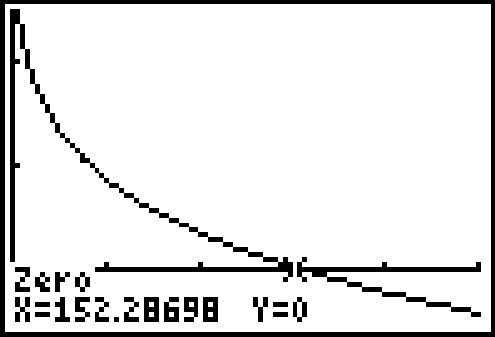
\includegraphics[width=1.75in]{./FurtherGraphics/WINDCHILL.jpg}}


\end{enumerate}

\item $9.8 \left(\dfrac{1}{4\pi}\right)^{2} \approx 0.062$ meters or $6.2$ centimeters

\item \begin{enumerate}

\item First rewrite the model as $P = 1.23x^{\frac{2}{5}}y^{\frac{3}{5}}$.  Then $300 = 1.23x^{\frac{2}{5}}y^{\frac{3}{5}}$ yields $y = \left( \dfrac{300}{1.23x^{\frac{2}{5}}} \right)^{\frac{5}{3}}$.  If $x = 100$ then $y \approx 441.93687$.

\end{enumerate}

\item \begin{enumerate}

\item $[0, c)$

\item $~$

\begin{tabular}{ll} 
$m(.1c) = \dfrac{m_{r}}{\sqrt{.99}} \approx 1.005m_{r}$ & $m(.5c) = \dfrac{m_{r}}{\sqrt{.75}} \approx 1.155m_{r}$\\ \smallskip

$m(.9c) = \dfrac{m_{r}}{\sqrt{.19}} \approx 2.294m_{r}$ & $m(.999c) = \dfrac{m_{r}}{\sqrt{.0.001999}} \approx 22.366m_{r}$ \\ \end{tabular}


\item As $x \rightarrow c^{-}, \, m(x) \rightarrow \infty$

\item If the object is traveling no faster than approximately $0.99995$ times the speed of light, then its observed mass will be no greater than $100m_{r}$.

\end{enumerate}


\item $k^{-1}(x) = \dfrac{x}{\sqrt{x^{2} - 4}}$

\item \begin{enumerate}

\item  $y = \frac{1}{3}x^{3/2} - \sqrt{x} + \frac{2}{3}$.  The point $\left(0,\frac{2}{3}\right)$ is when Fritzy's path crosses Chewbacca's path - in other words, where Fritzy catches Chewbacca.

\item $y = \frac{1}{6}x^3+\frac{1}{2x} - \frac{2}{3}$.  Using the techniques from Chapter \ref{Rationals}, we find as $x \rightarrow 0^{+}$, $y \rightarrow \infty$ which means, in this case, Fritzy's pursuit never ends;  he never catches Chewbacca. This makes sense since Chewbacca has a head start and is running faster than Fritzy.

\begin{center}

\begin{tabular}{cc}

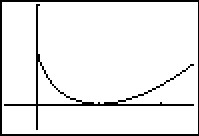
\includegraphics[width=2in]{./FurtherGraphics/PURSUIT01.jpg} & \hspace{1in} 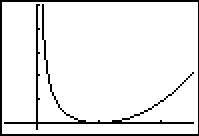
\includegraphics[width=2in]{./FurtherGraphics/PURSUIT02.jpg}  \\

$y = \frac{1}{3}x^{3/2} - \sqrt{x} + \frac{2}{3}$ & \hspace{1in} $y = \frac{1}{6}x^3+\frac{1}{2x} - \frac{2}{3}$ \\

\end{tabular}

\end{center}

\end{enumerate}


\end{enumerate}

\closegraphsfile


\end{document}